\documentclass[]{scrreprt}
\usepackage{amsmath,amsfonts,graphicx}
\usepackage{multirow}
\usepackage{pslatex}
\usepackage{tabularx}
\usepackage{comment}
\usepackage{xspace}
\usepackage{array}

\usepackage{hyperref}

\usepackage{caption}
\DeclareCaptionFont{white}{\color{white}}
\DeclareCaptionFormat{listing}{\colorbox{gray}{\parbox{\textwidth}{#1#2#3}}}

\graphicspath{
{figures/}
}

\newcommand{\uo}{\mbox{UO\textsubscript{2}}\xspace}

\setcounter{secnumdepth}{3}


\begin{document}


\title{Richards Tests}
\author{Andy Wilkins \\
CSIRO}
\maketitle

\tableofcontents

%%%
\chapter{Introduction}
%%%

The Richards' equation describes slow fluid flow through a porous
medium.  This document describes the test suite associated with the
Richards MOOSE code: both brief unit-style tests, and more complicated
benchmark verifications.  Many of the tests are run automatically
every time the code is updated.  Some of the tests are marked `heavy'
since they are more lengthy (they take over 2 seconds to run) and
these must be run manually.  There are two other accompanying documents:
(1) The theoretical and numerical foundations of the code, which also
describes the notation used throughout this document; (2) Examples of
input syntax that users can utilise when building models.

The test suite does not {\em prove} that the Richards' equation is
correctly implemented in MOOSE, as the expected results might be
obtained by pure luck.  At present around 90\% of C++
code are covered by the tests, with much of the remainder being
exception catching in object constructors (checking user input is
correctly formatted, etc).  The tests are ordered approximately by
complexity, so that by the end I hope that all readers will agree that
the implementation is highly likely to be correct.  The tests are as
follows.
\begin{itemize}
\item Chapter~\ref{uo} tests the so-called UserObjects that define the
 Richards' nonlinear functions: relative permeability, density, and
 effective saturation.  These functions are independent of the
 Darcy/Richards flow, but of course they must be correctly implemented
 in order that the code give correct solutions of flow problems.
\item Chapter~\ref{jac} contains many tests the Jacobian of Richards'
  flow.  The Jacobian actually has little effect on the final
  numerical solution of a flow problem, but if it is incorrectly
  implemented then MOOSE will display poor convergence
  characteristics.  Therefore it is extremely important to check the
  Jacobian.
\item Chapter~\ref{ma} checks that the fluid mass is calculated correctly.
\item Chapter~\ref{gh} contains many tests of the long-time behaviour
  in simple problems, which should just be hydrostatic pressure head,
  with the caveat that $S\geq S_{\mathrm{imm}}$.
\item Chapter~\ref{si} checks that the piecewise-linear sink and the
  half-Gaussian sink are implemented correctly.
\item Chapter~\ref{st} checks that the piecewise-linear stream-type
  sink (the PolyLineSink) is implemented correctly.
\item Chapter~\ref{pp} checks that pressure pulses diffuse correctly
  through a fully-saturated medium.
\item Chapter~\ref{nc} checks that MOOSE behaves correctly when the
  system contains a sink flux that is a function of porepressure.  A
  particular function is used so that an analytic solution exists.
\item Chapter~\ref{th} compares MOOSE with the Theis solution for
  extraction of fluid from a saturated aquifer.
\item Chapter~\ref{bh} demonstrates that boreholes are correctly
  implemented by comparing with the desired expression for the flux to
  the borehole, and by comparing with the known 2D analytic solution.
\item Chapter~\ref{bw} demonstrates that flow in the unsaturated
  region along with source fluxes is correctly implemented by comparing
  with the analytic solution of Broadbridge and White for constant
  infiltration.
\item Chapter~\ref{wli} demonstrates that flow in the unsaturated
  region is correctly implemented by comparing with the analytic
  solution of Warrick, Lomen and Islas for drainage of a medium under
  the action of gravity.
\item Chapter~\ref{forsyth} compares MOOSE with numerical results from
  HYDRUS for infiltration and drainage from a large caisson.  In
  reality, this is very similar to Chapters~\ref{bw} and~\ref{wli}:
  the only essential differences are the capillary and relative
  permeability functions.
\item Chapter~\ref{bl} compares a single-phase MOOSE simulation with
  the analytic solution of the Buckley-Leverett problem.
\item Chapter~\ref{ex} demonstrates that MOOSE yields the expected
  answer for a simulation containing an excavation.
\item Chapter~\ref{rsc} compares a two-phase MOOSE simulation with
  the analytic solution of water infiltration provided by Rogers, Stallybrass and Clements.
\item Chapter~\ref{bl2} compares a two-phase MOOSE simulation with
  the analytic solution of the Buckley-Leverett problem.
\end{itemize}


\chapter{UserObject tests}
\label{uo}

The Richards' UserObjects define the nonlinear functions that form the
core of all models.  The tests of these UserObjects involve checking
whether the functions and their derivatives are correctly coded.  This
is done by comparing the values of the UserObjects with
ParsedFunctions that are coded into a MOOSE input file, and the values
of the UserObject derivatives with finite-differences of the same
ParsedFunction.  These are simple tests and are part of the automatic
test suite.  The following tests are performed.

\begin{itemize}

\item That the `power' form of the relative permeability:
\begin{equation}
\kappa_{\mathrm{rel}}(S) = (n+1)S^{n} - nS^{n+1} \ ,
\end{equation}
is correctly coded, and also that its first and second derivatives
with repsect to $S$ are correctly coded.

\item That the `van Genuchten' form of the relative permeability:
\begin{equation}
\kappa_{\mathrm{rel}}(S) = \sqrt{S}\left(1 - \left(1 -
S^{1/m}\right)^{m}\right)^{2} \ ,
\end{equation}
is correctly coded, and also that its first and second derivatives
with respect to $S$ are correctly coded.

\item That the `modified van Genuchten' form of the relative permeability:
\begin{equation}
\kappa_{\mathrm{rel}}(S) = \left\{
\begin{array}{ll}
\sqrt{S}\left(1 - \left(1 -
S^{1/m}\right)^{m}\right)^{2} \ & \mbox{ for } S<S_{\mathrm{cut}} \\
\mbox{cubic} \ & \mbox{ for } S \geq S_{\mathrm{cut}}
\end{array}
\right.
\end{equation}
is correctly coded, and also that its first and second derivatives
with respect to $S$ are correctly coded.

\item That the `Broadbridge-White' form of the relative permeability:
\begin{equation}
\kappa_{\mathrm{rel}}(S) = \kappa_{n} +
(\kappa_{s}-\kappa_{n})\frac{\Theta^{2}(C-1)}{C-\Theta} \ ,
\label{bw.krel}
\end{equation}
where $\Theta = (S-S_{n})/(S_{s}-S_{n})$, 
is correctly coded, and also that its first and second derivatives
with respect to $S$ are correctly coded.  Broadbridge and White assume
that saturation is bounded $S_{n}\leq S\leq S_{s}$, so for most MOOSE
models it is appropriate to treat $S_{n}$ as the immobile saturation
with $\kappa_{n}=0$, and $S_{s}=1$ with $\kappa_{s}=1$.

\item That the `monomial' form of the relative permeability:
\begin{equation}
\kappa_{\mathrm{rel}}(S) = S^{n} \ ,
\end{equation}
is correctly coded, and also that its first and second derivatives
with repsect to $S$ are correctly coded.

\item That the `powergas' form of the relative permeability:
\begin{equation}
\kappa_{\mathrm{rel}}(S) = 1 - (n+1)(1-S)^{n} + n(1-S)^{n+1} \ ,
\end{equation}
is correctly coded, and also that its first and second derivatives
with repsect to $S$ are correctly coded.


\item That the `constant bulk modulus' form of the density
\begin{equation}
\rho(P) = \rho_{0}e^{P/B} \ ,
\end{equation}
is correctly coded, and also that its first and second derivatives
with respect to $P$ are correctly coded.

\item That the `ideal gas' form of the density
\begin{equation}
\rho(P) = s(P-P_{\mathrm{0}}) \ ,
\end{equation}
is correctly coded, and also that its first and second derivatives
with respect to $P$ are correctly coded.

\item That the density of methane (kg.m$^{-3}$) at 20degC as a
  function of $P$ (Pa): 
\begin{equation}
\rho(P) = 6.54576947608\times 10^{-6}P + 1.04357716547\times 10^{-13} P^{2}
\end{equation}
is correctly coded, and also that its first and second derivatives
with respect to $P$ are correctly coded.

\item That the `van Genuchten' effective saturation
\begin{equation}
S_{\mathrm{eff}} = \left(1 + (\alpha
P_{\mathrm{c}})^{\frac{1}{1-m}}\right)^{-m} \ ,
\end{equation}
is correctly coded, and also that its first and second derivatives
with respect to $P_{\mathrm{c}}$ are correctly coded.

\item That the `Broadbridge-White' effective saturation valid for
  small $\kappa_{n}$, defined by
\begin{equation}
\frac{P_{\mathrm{c}}}{\lambda_{s}} = \frac{1-\Theta}{\Theta} - \frac{1}{C}\log
\left( \frac{C-\Theta}{(C-1)\Theta} \right) \ ,
\end{equation}
with $\Theta = (S_{\mathrm{eff}} - S_{n})/(S_{s}-S_{n})$, 
is correctly coded, and also that the first and second derivatives of
$S_{\mathrm{eff}}$ with respect to $P_{\mathrm{c}}$ are correctly
coded.  Note that Broadbridge and White assume that
$S_{\mathrm{eff}}=S$ (no residual saturations) and $S_{n}\leq S \leq
S_{s}$, so in most MOOSE models $S_{n}$ is the immobile saturation.

\item That the `Rogers-Stallybrass-Clements' effective saturation,
  valid for zero residual saturations and oil viscosity double that of
  water viscosity, defined by
\begin{equation}
S_{\mathrm{eff}} = \frac{1}{\sqrt{1 +
    \exp\left(\frac{P_{\mathrm{c}}-P_{\mathrm{shift}}}{P_{\mathrm{scale}}}\right)}}
\ ,
\end{equation}
and its derivatives with respect to $P_{\mathrm{c}}$ are correctly coded.


\end{itemize}



\chapter{Jacobian tests}
\label{jac}

The UserObjects and their derivatives need to be combined to form a
residual and a Jacobian during the solution process.  Correctly coding
the Jacobian leads to rapid convergence to the correct solution, so
tests of the Jacobian are important.  These are simple tests and are
part of the automatic test suite.

In MOOSE parlance, the Jacobian consists of `Diagonal' and
`OffDiagonal' terms.  The former consist of the derivative of a
variable's residual with respect to the same variable (at the same
quadrature point or a different one); while the latter
consist of the derivatives with respect to another variable (at the
same quadrature point or a different one).

The `Diagonal' terms are tested using a single-phase single-element
model with random initial conditions.  Sixteen different tests are
performed which are all possible combinations of:
\begin{itemize}
\item Fully-saturated or unsaturated initial conditions
\item With or without gravity
\item With or without SUPG
\item With or without unlumped time derivatives
\end{itemize}
Of course, the unsaturated case with gravity, SUPG and time
derivatives is the most complicated, but the other cases are useful
for debugging.  In addition, the Jacobian of the lumped time derivative is checked.

The `OffDiagonal' terms only appear if there is more than one pressure
variable, that is for multi-phase problems.  A two-phase
single-element model is used with random initial conditions
obeying the constraint $P_{1}\geq P_{2}$ (to be meaningful physically).  Eight
different tests are performed which model all possible combinations
of:
\begin{itemize}
\item With or without gravity
\item With or without SUPG
\item With or without unlumped time derivatives
\end{itemize}
Two other tests are also performed: the first with random initial
conditions subject to $P_{1}=P_{2}$ so that the system is fully
saturated with the ``1'' phase; and the second with random initial
conditions subject to $P_{1}\ll P_{2}$ so the system is almost fully
saturated with the ``2'' phase.

In addition to these tests, a lumped time derivative is used in three
two-phase tests: with gravity and SUPG; with gravity, SUPG and fully
saturated with the ``1'' phase; with gravity and SUPG and almost fully
saturated with the ``2'' phase.

In addition to these tests, the Jacobians for the following sinks/sources are tested:
\begin{itemize}
\item Piecewise linear sink
\item Half Gaussian sink
\item Polyline stream sink
\end{itemize}



\chapter{Fluid mass}
\label{ma}

The total fluid mass within a volume $V$ is
\begin{equation}
\int_{V} \phi\rho S \ .
\end{equation}
It must be checked that MOOSE calculates this correctly in order that
mass-balances be correct, and also because this quantity is used in a
number of tests below.

A 1D model with $-1\leq x \leq 1$, and with two elements of size 1 is
created with the following properties:
\begin{center}
\begin{tabular}{|ll|}
\hline
Constant fluid bulk modulus & 1\,Pa \\
Fluid density at zero pressure & 1\,kg.m$^{-3}$ \\
Residual fluid saturation & 0.1 \\
Residual air saturation & 0.1 \\
Van Genuchten $m$ & 0.5 \\
Van Genuchten $\alpha$ & 1\,Pa$^{-1}$ \\
Porosity & 0.1 \\
\hline
\end{tabular} 
\end{center}
The porepressure is set at $P=x$.

For linear-lagrange elements, MOOSE calculates the integral over
$-1\leq x \leq 1$ by performing a sum over quadrature points at
$x=\pm 0.788675$ and $x=\pm 0.211325$.
Using the properties given above, this yields:
\begin{center}
\begin{tabular}{|cccccc|}
\hline
$x$ & $p$ & Density & $S_{\mathrm{eff}}$ & Saturation & Mass \\
\hline
-0.788675 & -0.788675 & 0.454447 & 0.785188 & 0.72815 & 0.016545 \\
-0.211325 & -0.211325 & 0.809511 & 0.978392 & 0.882714 & 0.035728 \\
0.211325 & 0.211325 & 1.235314 & 1 & 0.9 & 0.055589 \\
0.788675 & 0.788675 & 2.200479 & 1 & 0.9 & 0.099022 \\
\hline
 & & & & Total & 0.206884 \\
\hline
\end{tabular} 
\end{center}
MOOSE also gives the total mass as 0.206884\,kg.  This test is part of
the automatic test suite that is run every time the code is updated.

Since the same computer code is used for single and multi phase
simulations, the fluid mass does not need to be checked for anything
other than the single-phase case.





\chapter{Long-time behaviour}
\label{gh}

These tests concern the steadystate pressure distribution obtained
either by running a transient model for a long time, or by running a
steady-state analysis, both of which should lead to the same result.
Without fluxes, the steadystate pressure distribution is just
\begin{equation}
P(x) = P_{0} - \rho_{0} g x \ ,
\end{equation}
if the fluid bulk modulus, $B$, is large enough compared with $P$, otherwise
\begin{equation}
P(x) = -B \log\left( e^{-P_{0}/B} + \frac{g\rho_{0}x}{B} \right) \ .
\label{grav.head.eqn}
\end{equation}
Here I am assuming the density is given by $\rho = \rho_{0}e^{-P/B}$
with constant bulk modulus, $g$ is the
magnitude acceleration due to gravity (a vector assumed to be pointing in the
negative $x$ direction), and $x$ is position.  The tests described below
are simple tests and are part of the automatic test suite.

This is verified by running sixteen single-phase single-element models
with random initial conditions.  The sixteen cases are all possible
combinations of:
\begin{itemize}
\item Fully-saturated or unsaturated initial conditions
\item With or without gravity
\item With or without SUPG
\item Transient or Steadystate
\end{itemize}
Eight two-phase simulations are also run.  These are also
single-element models, but with initial conditions that ensure the
saturations of the phases are between 0.3 and 0.7.  These eight cases
are all possible combinations of:
\begin{itemize}
\item With or without gravity
\item With or without SUPG
\item Transient or Steadystate
\end{itemize}
A test with gravity and SUPG using the lumped time derivative is also run.
In the two-phase situation, Eqn~(\ref{grav.head.eqn}) must hold for
each phase, and the constant $P_{0}$ for each phase is determined
through conservation of mass of each phase.  (In the steadystate
situation, conservation of mass is meaningless, so $P_{0}$ is
arbitrary, but Eqn~(\ref{grav.head.eqn}) must still hold.)


\noindent In addition to these cases, a number of more complicated scenarios are
also part of the automatic test suite:
\begin{enumerate}
\item\label{gh20.item} A single-phase situation with nonzero immobile saturation.
  There are 5 elements in the $x$ direction along which gravity acts.
  The $x$ direction has length 20\,m, and the initial condition is
  sufficiently unsaturated so that after some time the saturation at
  the `top' of the model ($x\sim 20$) would reduce below immobile
  saturation if the relative permeability weren't preventing it.  Two
  cases are studied: with SUPG and without SUPG.  The results are
  shown in the top two pictures of Figure~\ref{gh.fig} and show that
  SUPG reduces oscillations and prevents $S<S_{\mathrm{imm}}$ in this
  example at least.
\item The same situation is in item~\ref{gh20.item}, but with 50
  elements in the $x$ direction.  Figure~\ref{gh.fig} shows once again
  the stabilising nature of SUPG is seen, as well as the hydrostatic
  pressure head for $S>S_{\mathrm{imm}}$.
\item A two-phase situation that starts with $P_{1}=P_{2}$, that is
  fully saturated.  A single element is used, along with gravity,
  SUPG, and transient analysis.  Three simulations are performed:
\begin{enumerate}
\item with an unlumped time derivative
\item with a lumped time derivative
\item using a {\tt RichardsMultiphaseProblem} object to maintain the
  bound $P_{2}\geq P_{1}$.
\end{enumerate}
These simulations checks that the MOOSE
  implementation yields the correct long-time behaviour for
  fully-saturated two-phase simulations.
\item A two-phase simulation with nonzero immobile saturations for
  both phases.  Both the unlumped time derivative and lumped time
  derivative are tested The automatic test suite contains 20-element
  versions, and the results are shown in Figure~\ref{gh2.fig}, along
  with the results from a 200-element version.  This figure
  demonstrates the reduction in spurious oscillations obtained by
  using a lumped time derivative.
\end{enumerate}

\begin{figure}[htb]
\centering
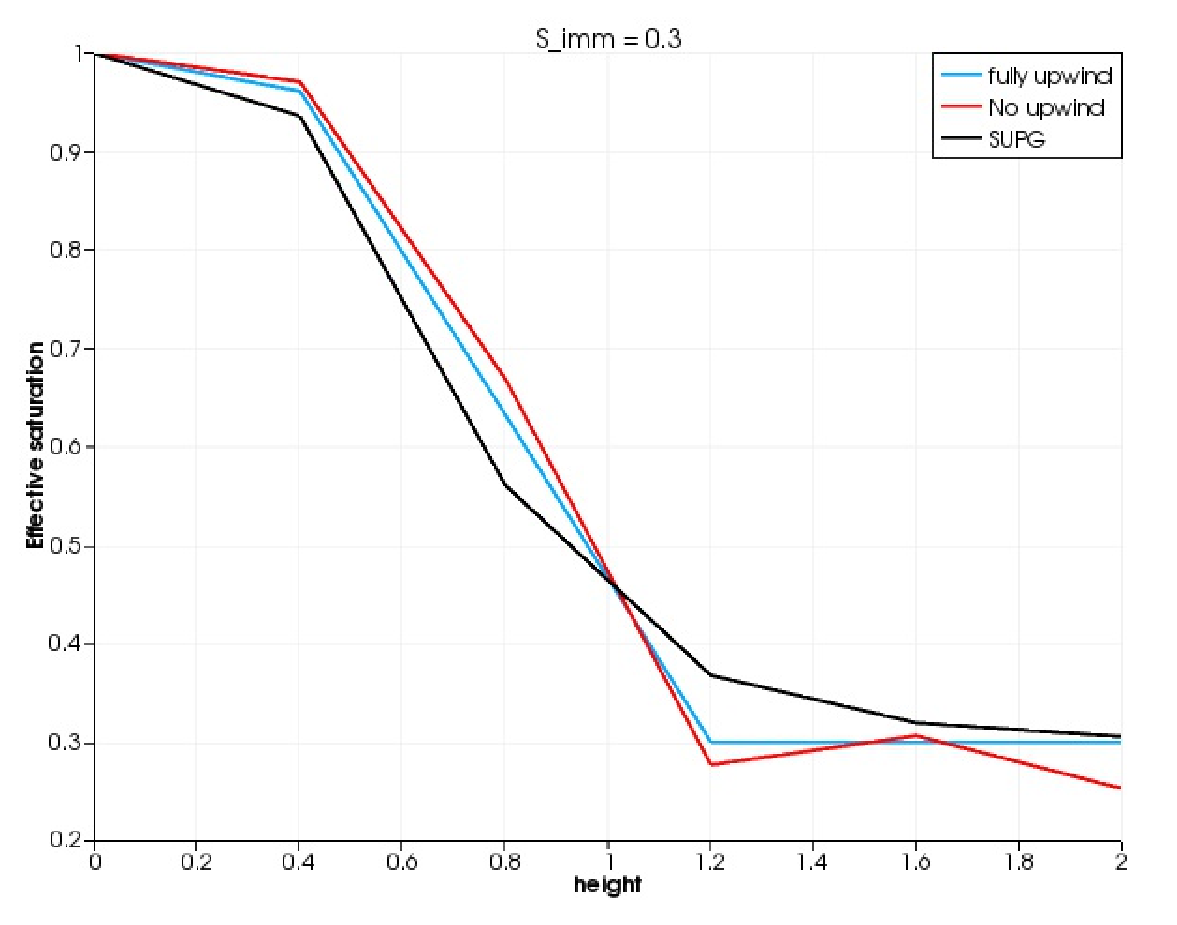
\includegraphics[width=10cm]{gh_seff.eps} \\
$\mbox{}$ \\
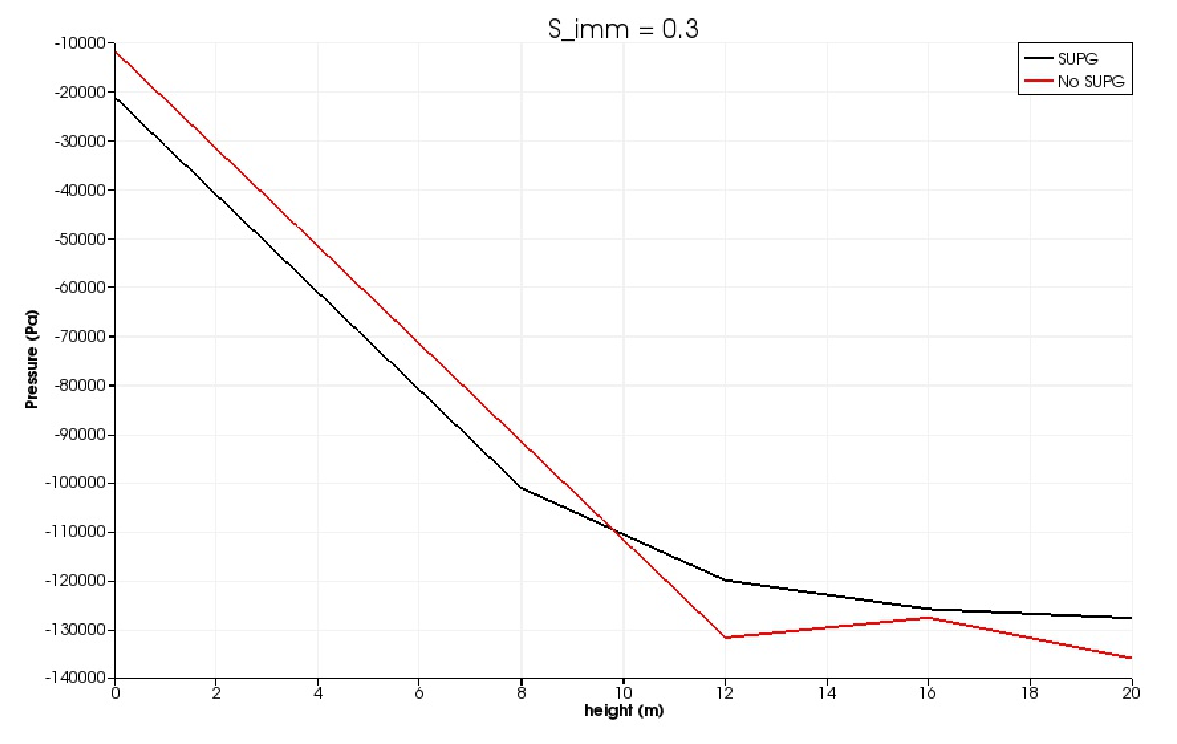
\includegraphics[width=10cm]{gh_p.eps} \\
$\mbox{}$ \\
\begin{tabular}{cc}
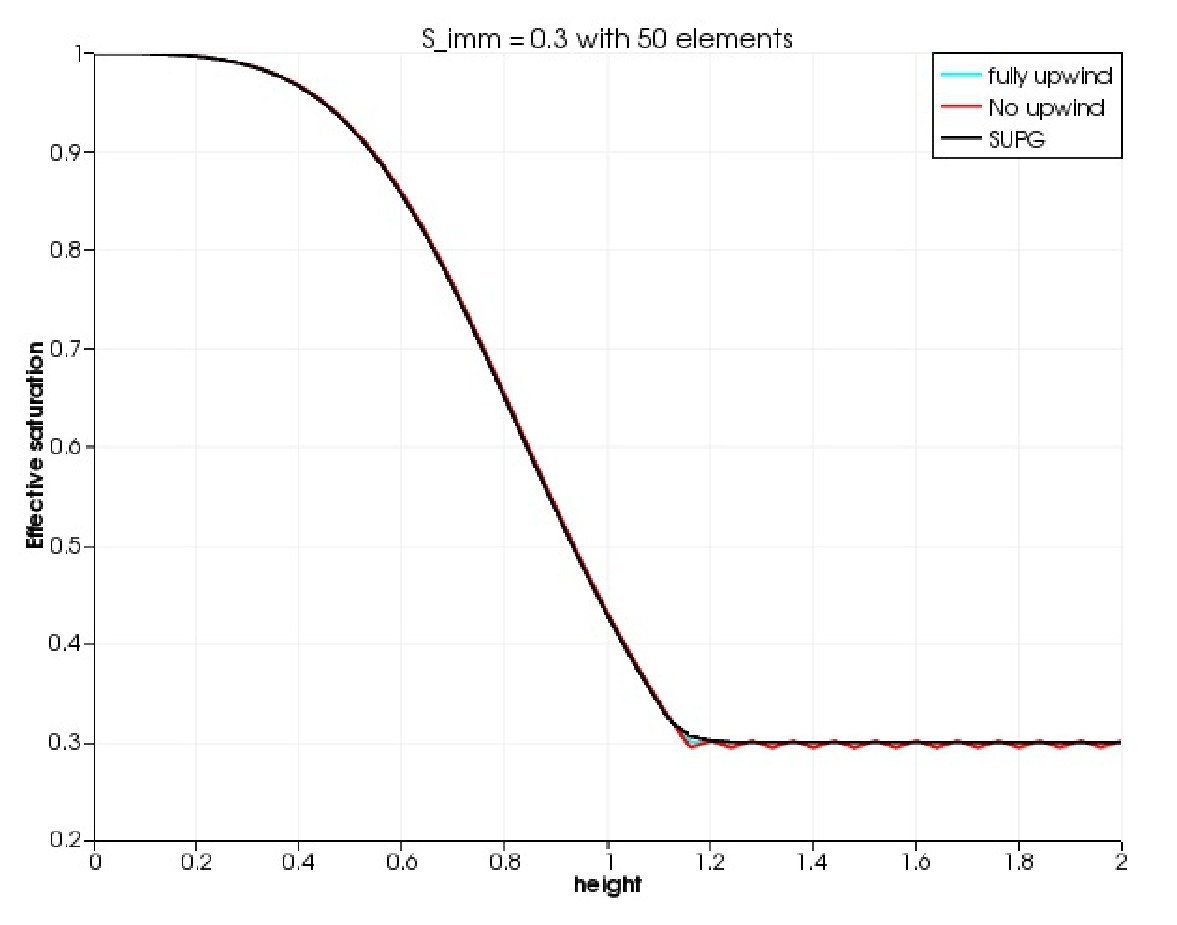
\includegraphics[width=8cm]{gh_seff_50.eps} &
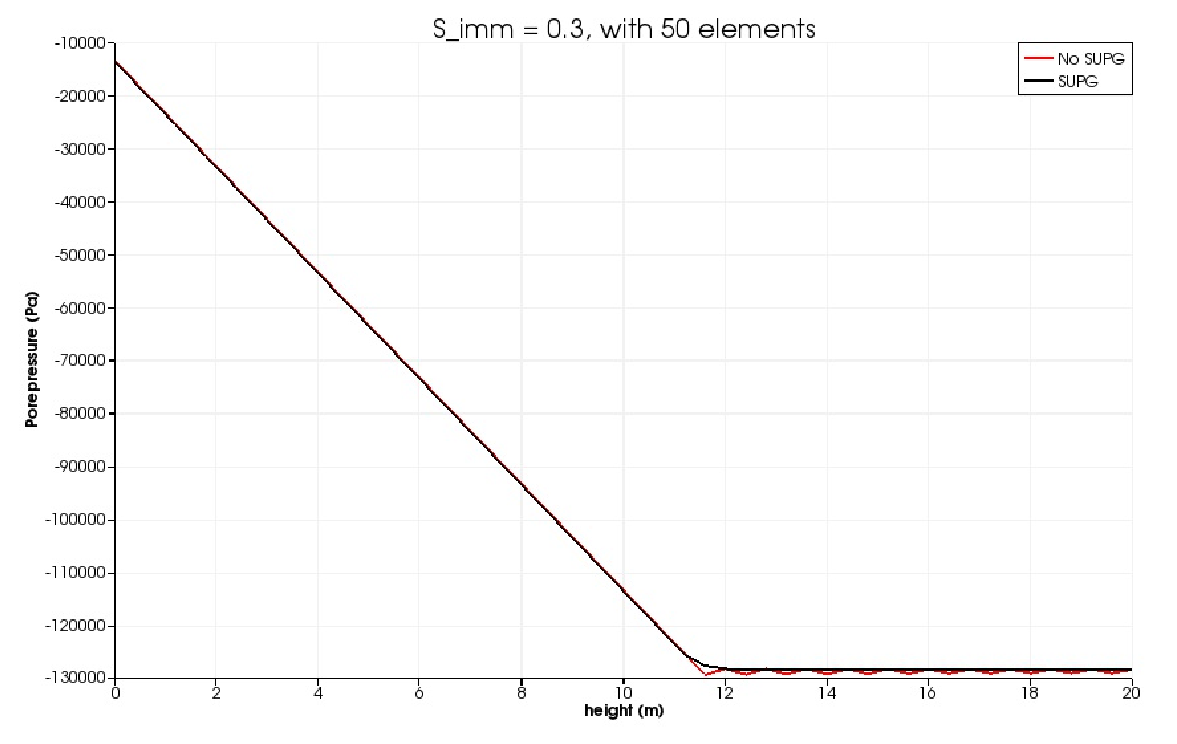
\includegraphics[width=8cm]{gh_p_50.eps} 
\end{tabular}
\caption{Results for $S_{\mathrm{imm}}=0.3$.  Gravity points to the
  left.  Top picture: Effective saturation.  Middle picture: Pore
  pressure.  Bottom pictures: The situation with 50 elements in the
  $x$ direction instead of just 5.  In each picture the red line is
  without SUPG, and oscillatory results can be observed in addition to
  $S_{\mathrm{eff}}< S_{\mathrm{imm}}$.}
\label{gh.fig}
\end{figure}

\begin{figure}[htb]
\centering
\begin{tabular}{cc}
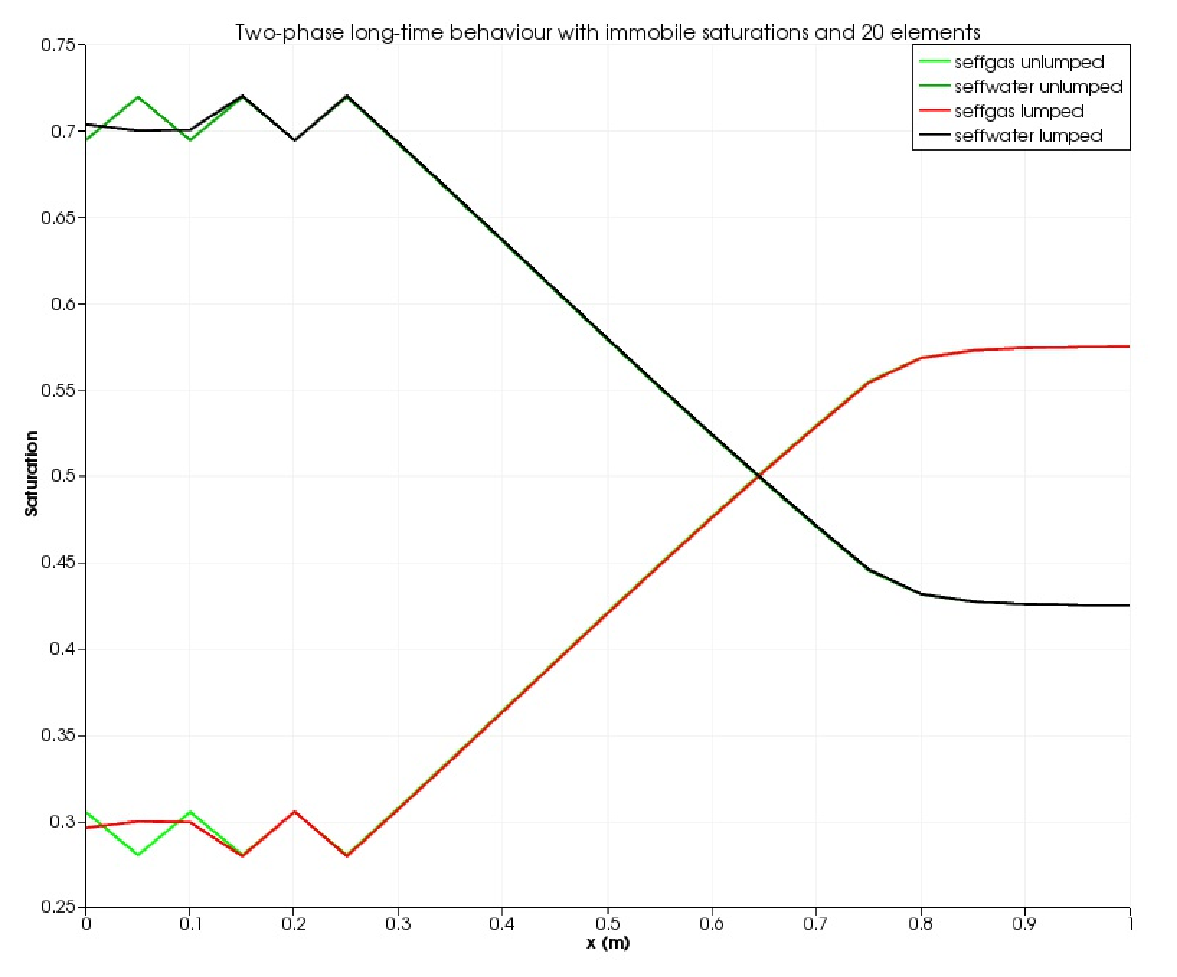
\includegraphics[width=8cm]{gh2_20.eps} &
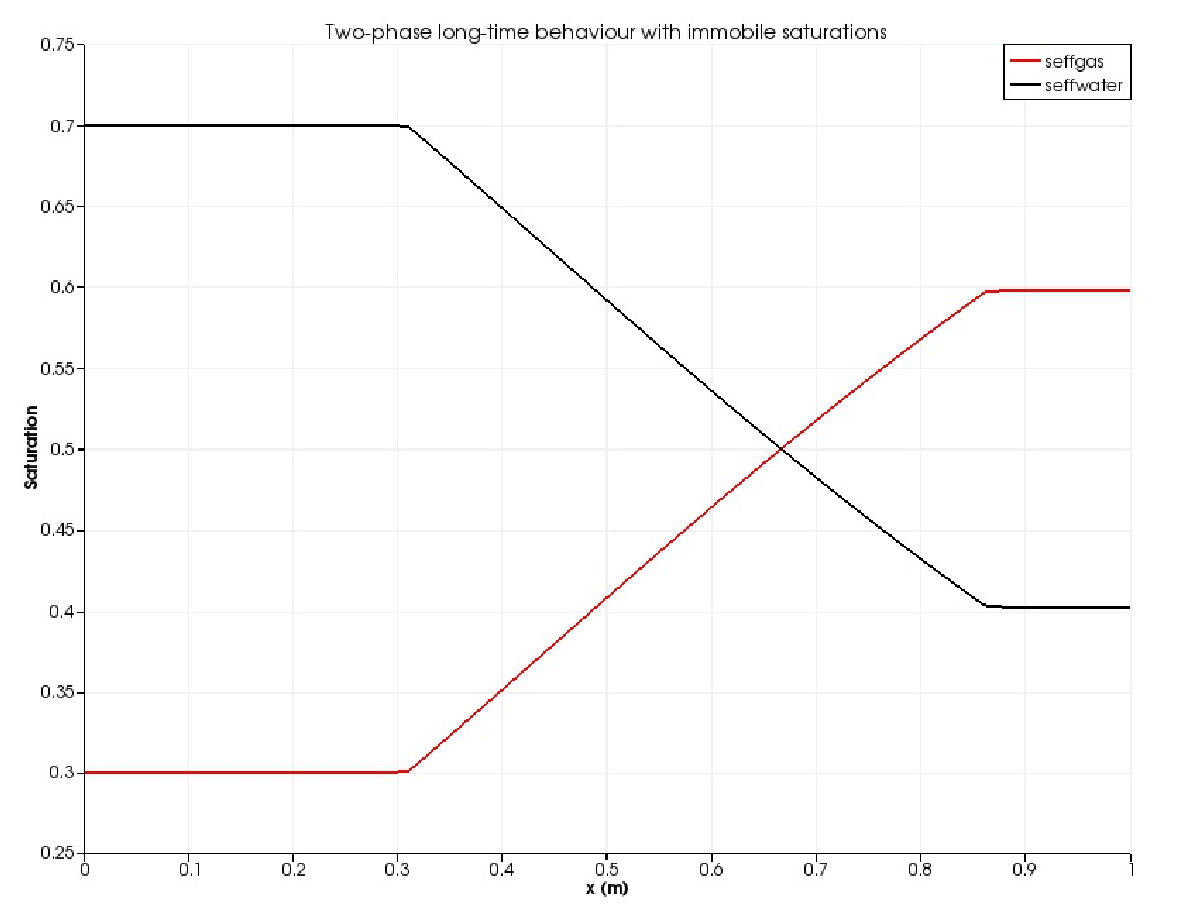
\includegraphics[width=8cm]{gh2.eps}
\end{tabular}{cc}
\caption{Two-phase long-time results for
  $S^{\mathrm{gas}}_{\mathrm{imm}}=0.3$ and
  $S^{\mathrm{water}}_{\mathrm{imm}}=0.4$.  Left: 20-element
  simulation with and without time-derivative lumping.  Right: 200-element simulation.}
\label{gh2.fig}
\end{figure}


\chapter{Piecewise linear and half-Gaussian sinks}
\label{si}

The MOOSE implementation allows users to specify sinks and sources
acting at boundaries that are functions of porepressure.  This chapter
tests that these sinks and sources act as specified.  These tests are
part of the automatic test suite that is run every time the code is
updated.

A 2D model with $0\leq x \leq 1$ and $0\leq y \leq 1$ with just a
single element is subjected to sink fluxes from its left and right
boundaries.  Because it is a single element no fluid flow within the
element occurs.  The following fluid properties are used:
\begin{center}
\begin{tabular}{|ll|}
\hline
Constant fluid bulk modulus & 1\,Pa \\
Fluid density at zero pressure & 1\,kg.m$^{-3}$ \\
Residual fluid saturation & 0.1 \\
Residual air saturation & 0.1 \\
Van Genuchten $m$ & 0.5 \\
Van Genuchten $\alpha$ & 1\,Pa$^{-1}$ \\
Power-type relative permeabilty $n$ & 2 \\
$\kappa_{xx}$ & $10^{-5}$\,m$^{2}$ \\
Porosity & 0.1 \\
\hline
\end{tabular} 
\end{center}

\noindent In the first test a piecewise-linear sink is applied with strength:
\begin{equation}
\mbox{sink flux (kg.m$^{-1}$.s$^{-1}$)} = \left\{
\begin{array}{ll}
1 & \mbox{ for } p \leq 0 \\
1+p & \mbox{ for } 0<p<1 \\
2 & \mbox{ for } p\geq 1 
\end{array}
\right.
\label{eqn.s01}
\end{equation}
The sink flux is recorded by into a Postprocessor by MOOSE.  It is
remotely possible that the MOOSE implementation {\em applies} the sink
flux incorrectly, but {\em records} it as a Postprocessor correctly as
specified by Eqn~(\ref{eqn.s01}).  Therefore the simulation also
records the fluid mass and mass-balance error in order to check that
the fluid mass is indeed being reduced correctly by the sink flux.
The initial condition is $p=2$\,Pa, and the simulation is run for
0.2\,s with 100 time steps.  The expected behaviour is demonstrated in
Figure~\ref{s01.fig}.

\begin{figure}[htb]
\centering
\begin{tabular}{cc}
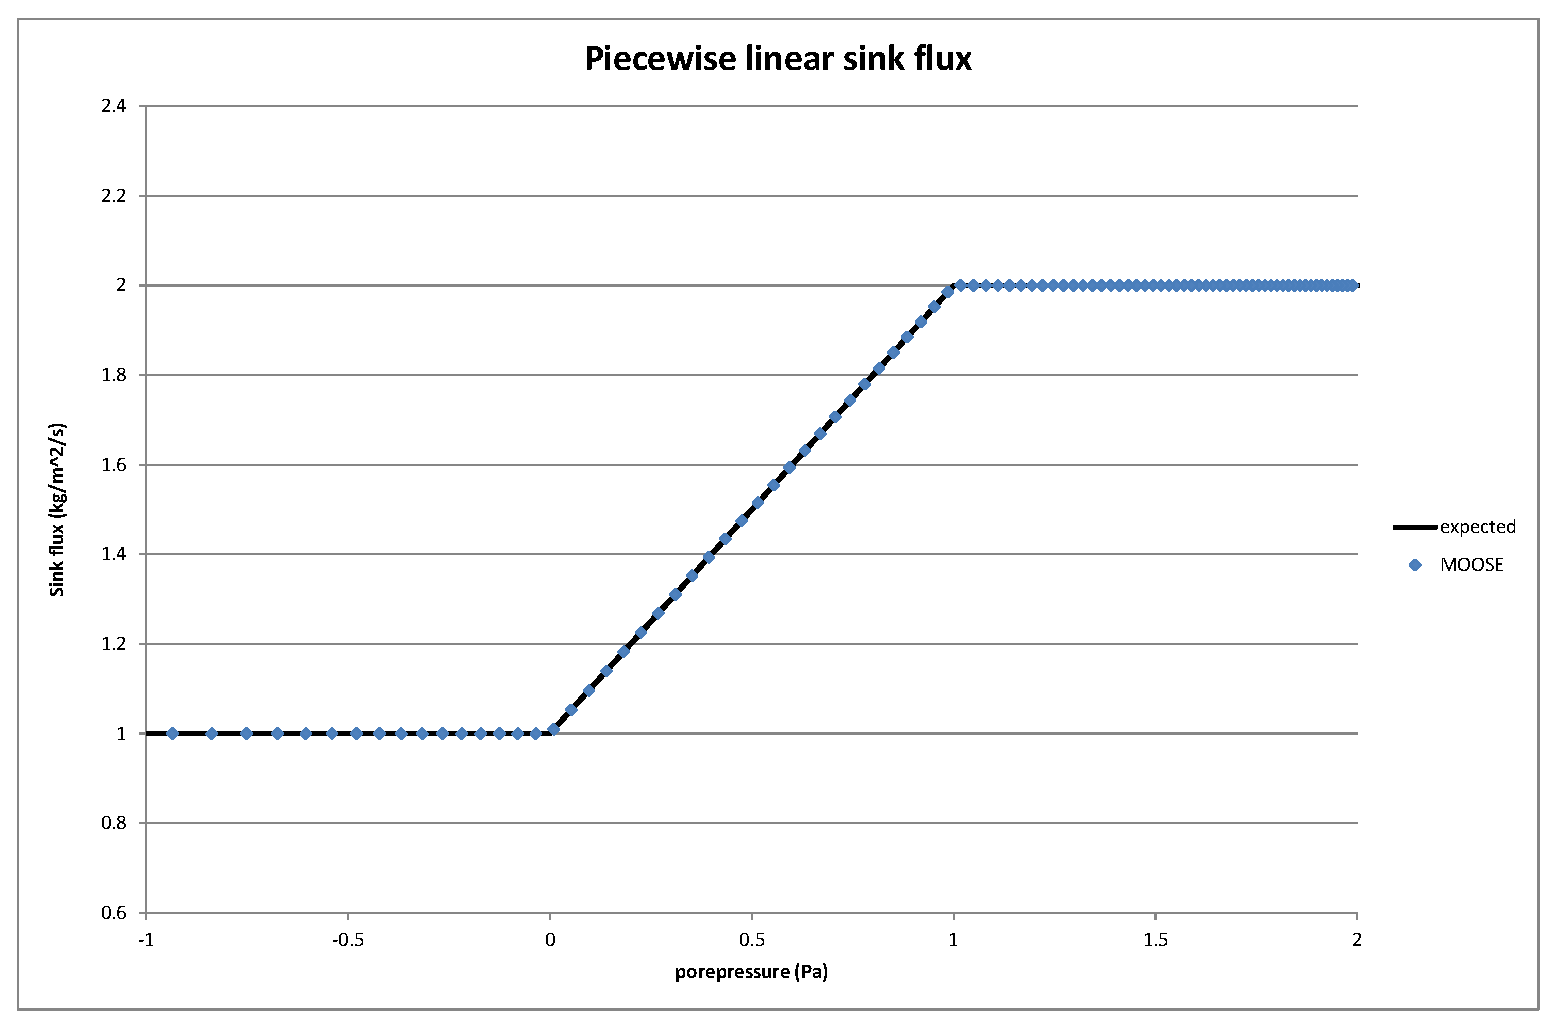
\includegraphics[width=7cm]{s01.eps} &
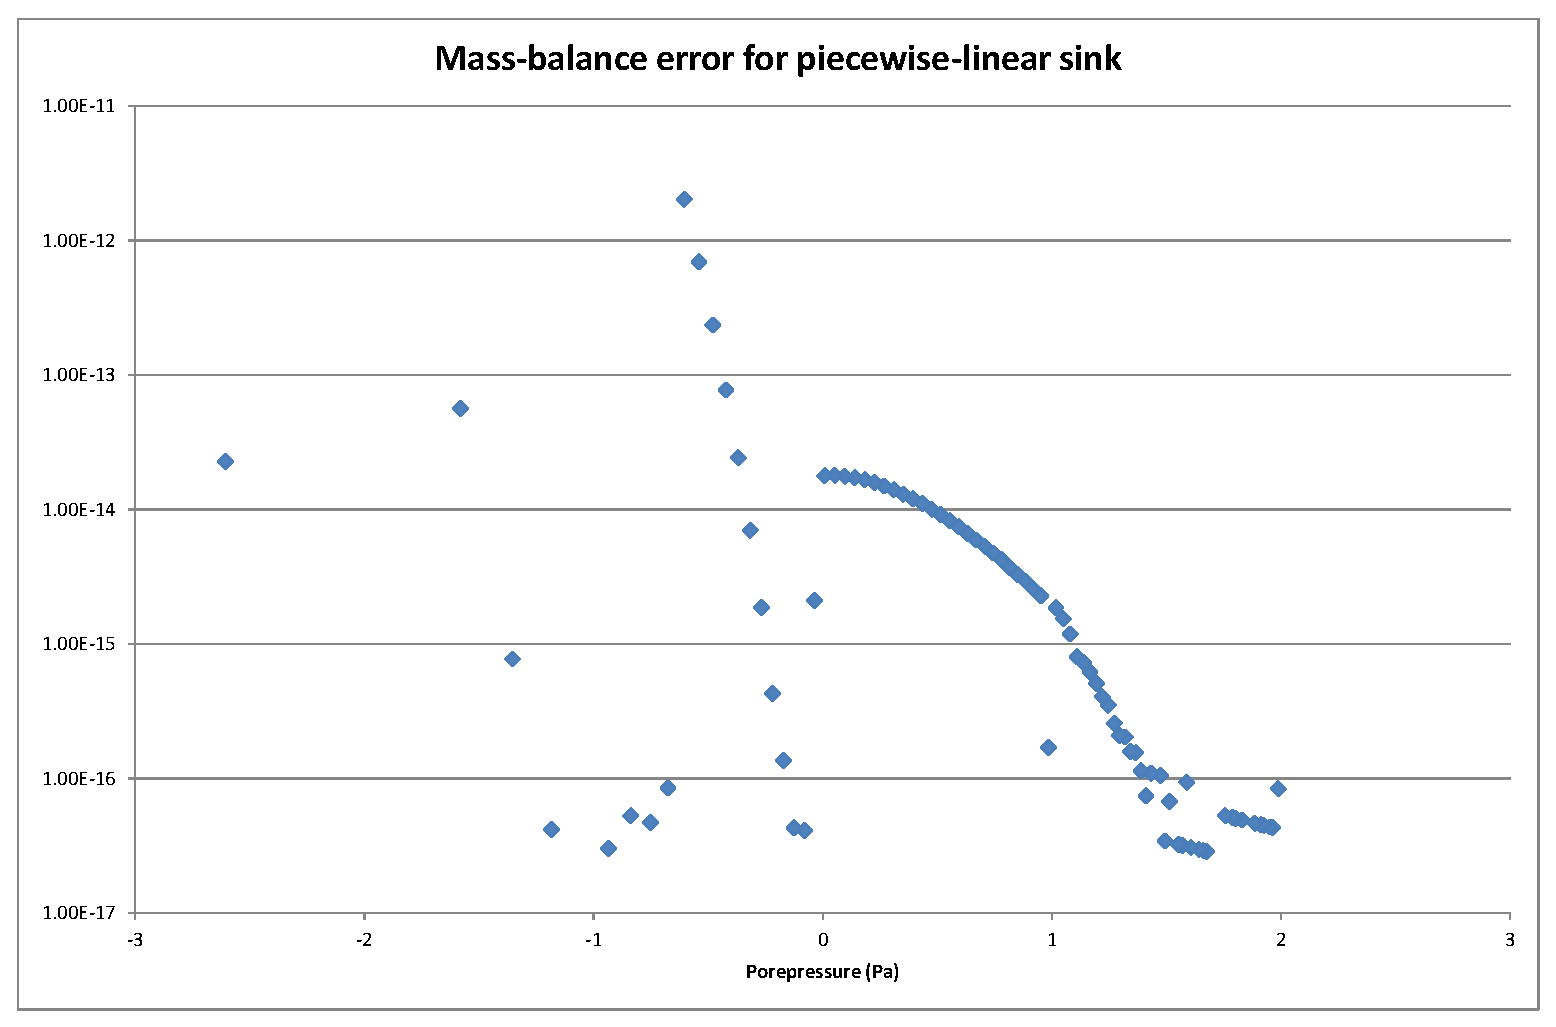
\includegraphics[width=7cm]{s01_mass_bal.eps}
\end{tabular}
\caption{Left: Comparison between the MOOSE result (in dots), and the
  expected behaviour of the sink flux given by Eqn~(\ref{eqn.s01}).
  Right: The mass-balance error is small for the simulation described
  demonstrating that the recorded sink flux is truly reducing the mass
  in the correct way.}
\label{s01.fig}
\end{figure}


\noindent In the second test a piecewise-linear sink is applied with strength:
\begin{equation}
\mbox{sink flux (kg.m$^{-1}$.s$^{-1}$)} = \left\{
\begin{array}{ll}
2\exp(-0.5(P-1)^{2}) & \mbox{ for } p < 1 \\
2 & \mbox{ for } p\geq 1 
\end{array}
\right.
\label{eqn.s02}
\end{equation}
This is called a half-Gaussian sink flux and may be used to model
evapotranspiration.  The sink flux is recorded by into a Postprocessor by MOOSE.  It is
remotely possible that the MOOSE implementation {\em applies} the sink
flux incorrectly, but {\em records} it as a Postprocessor correctly as
specified by Eqn~(\ref{eqn.s02}).  Therefore the simulation also
records the fluid mass and mass-balance error in order to check that
the fluid mass is indeed being reduced correctly by the sink flux.
The initial condition is $p=2$\,Pa, and the simulation is run for
0.4\,s with 100 time steps.  The expected behaviour is demonstrated in
Figure~\ref{s02.fig}.

\begin{figure}[htb]
\centering
\begin{tabular}{cc}
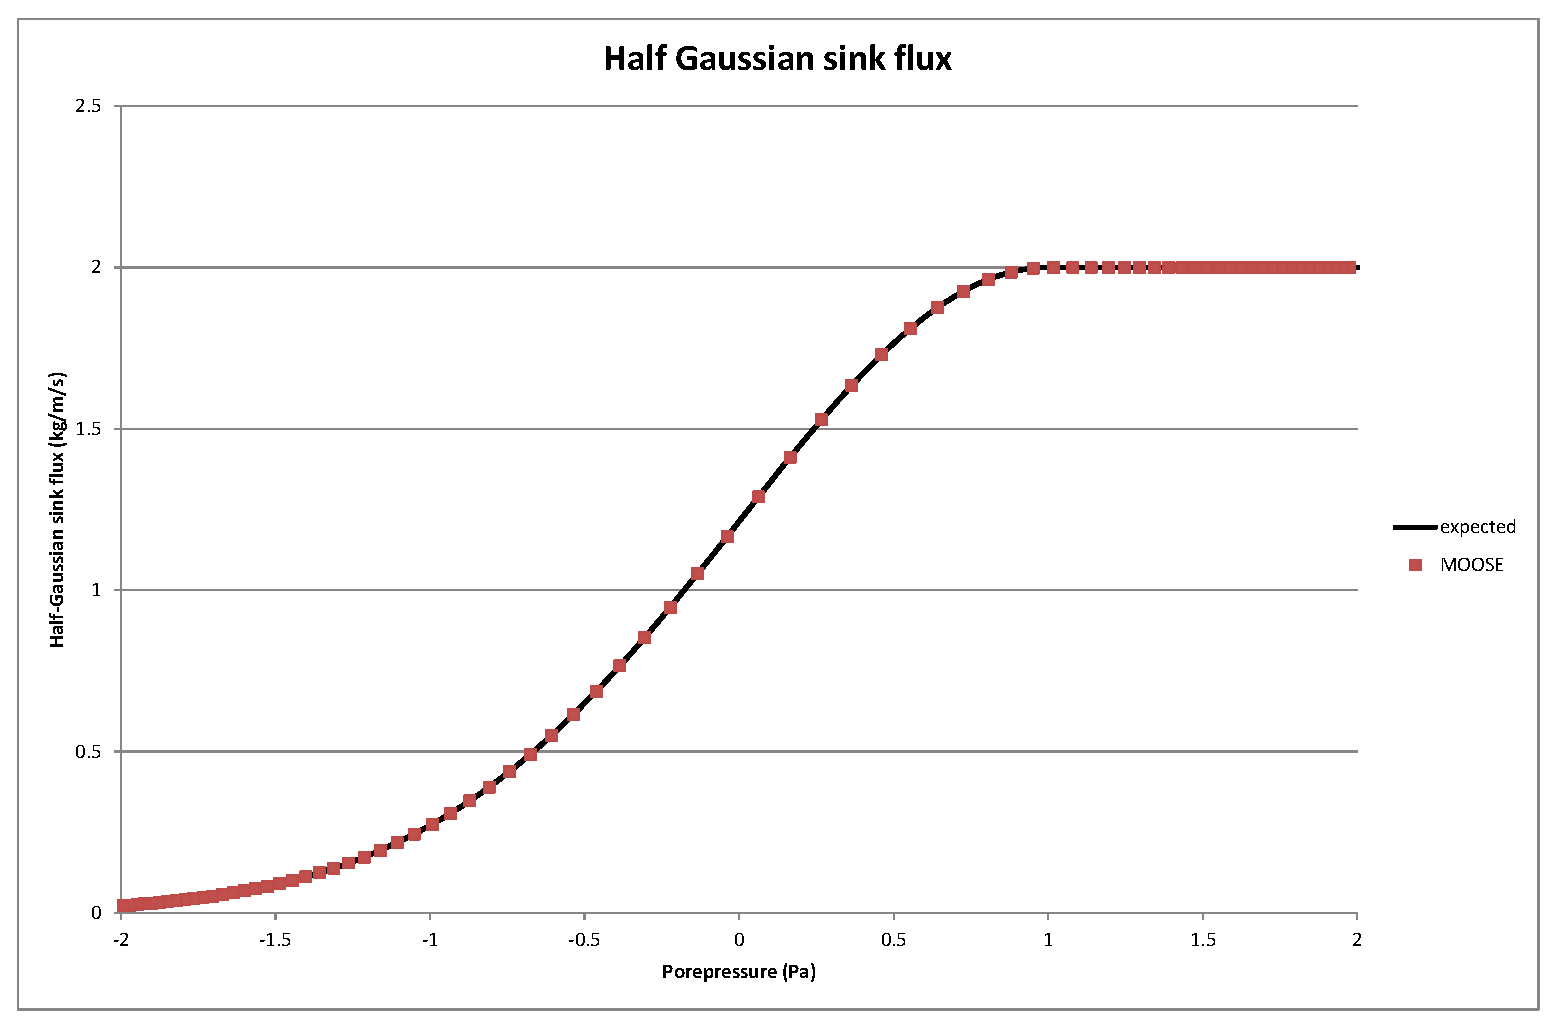
\includegraphics[width=7cm]{s02.eps} &
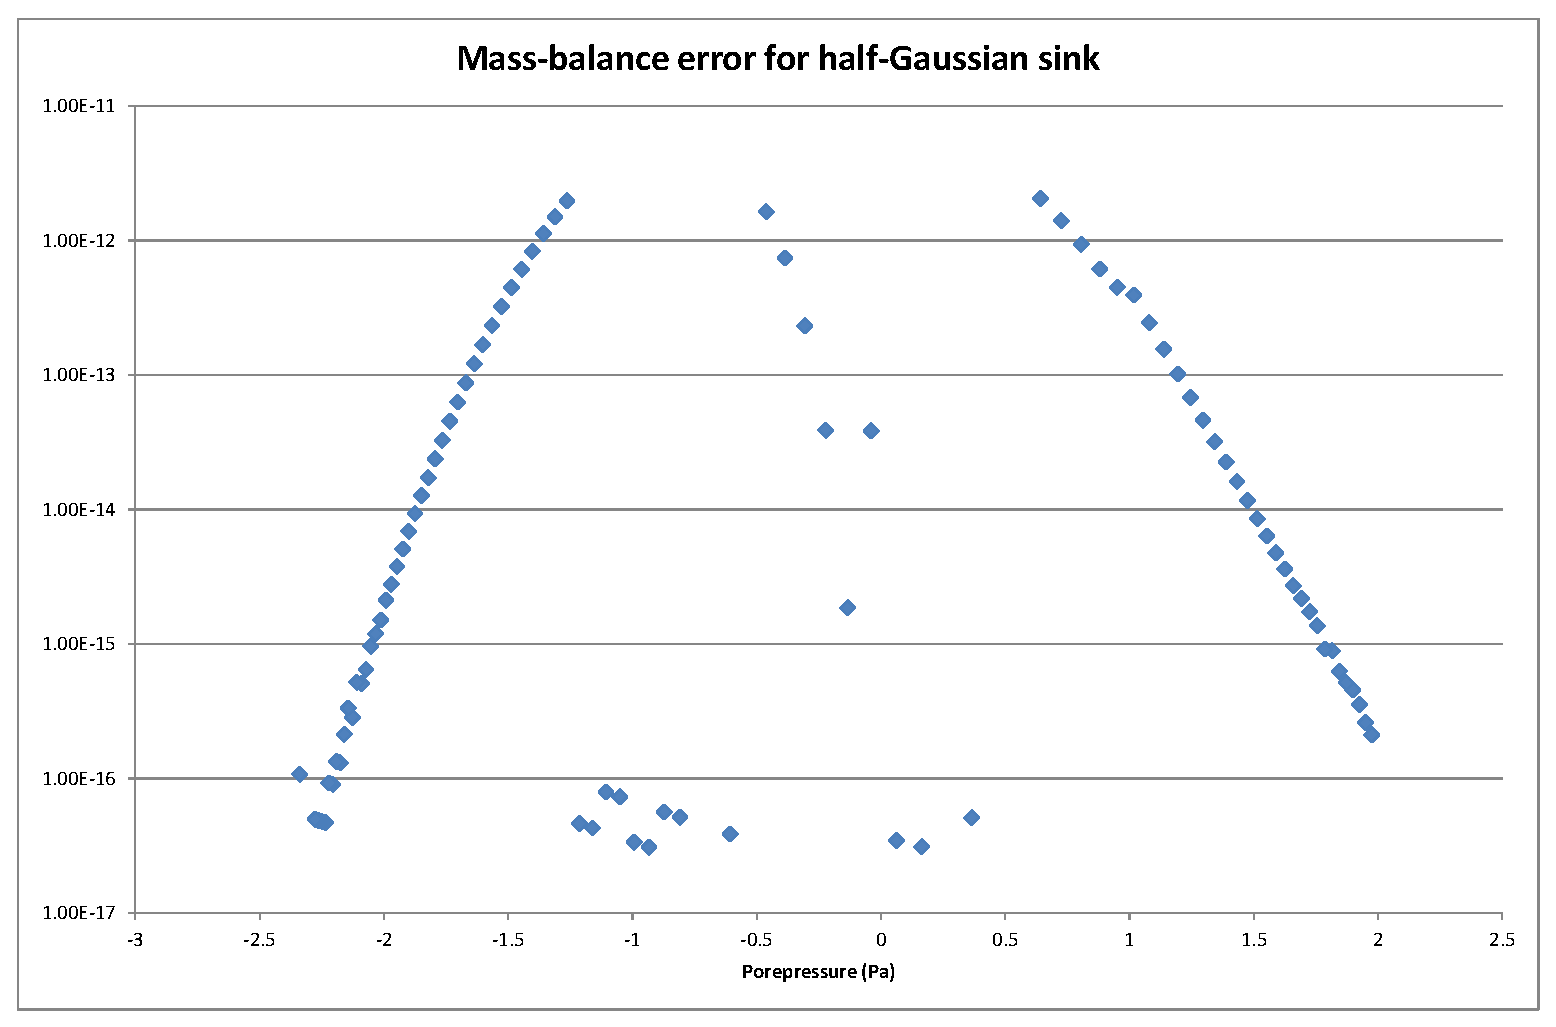
\includegraphics[width=7cm]{s02_mass_bal.eps}
\end{tabular}
\caption{Left: Comparison between the MOOSE result (in dots), and the
  expected behaviour of the sink flux given by Eqn~(\ref{eqn.s02}).
  Right: The mass-balance error is small for the simulation described
  demonstrating that the recorded sink flux is truly reducing the mass
  in the correct way.}
\label{s02.fig}
\end{figure}


\noindent In the third test a piecewise-linear sink with relative
permeability and mobility affects is used.  The flux strength is:
\begin{equation}
\mbox{sink flux (kg.m$^{-1}$.s$^{-1}$)} = 
\frac{\rho\kappa_{xx}\kappa_{\mathrm{rel}}}{\mu}
\times \left\{
\begin{array}{ll}
100 & \mbox{ for } p \leq -1 \\
150+50p& \mbox{ for } -1<p<1 \\
200 & \mbox{ for } p\geq 1 
\end{array}
\right.
\label{eqn.s03}
\end{equation}
The sink flux is recorded by into a Postprocessor by MOOSE.  It is
remotely possible that the MOOSE implementation {\em applies} the sink
flux incorrectly, but {\em records} it as a Postprocessor correctly as
specified by Eqn~(\ref{eqn.s03}).  Therefore the simulation also
records the fluid mass and mass-balance error in order to check that
the fluid mass is indeed being reduced correctly by the sink flux.
The initial condition is $p=2$\,Pa, and the simulation is run for
0.2\,s with 100 time steps.  The expected behaviour is demonstrated in
Figure~\ref{s03.fig}.

\begin{figure}[htb]
\centering
\begin{tabular}{cc}
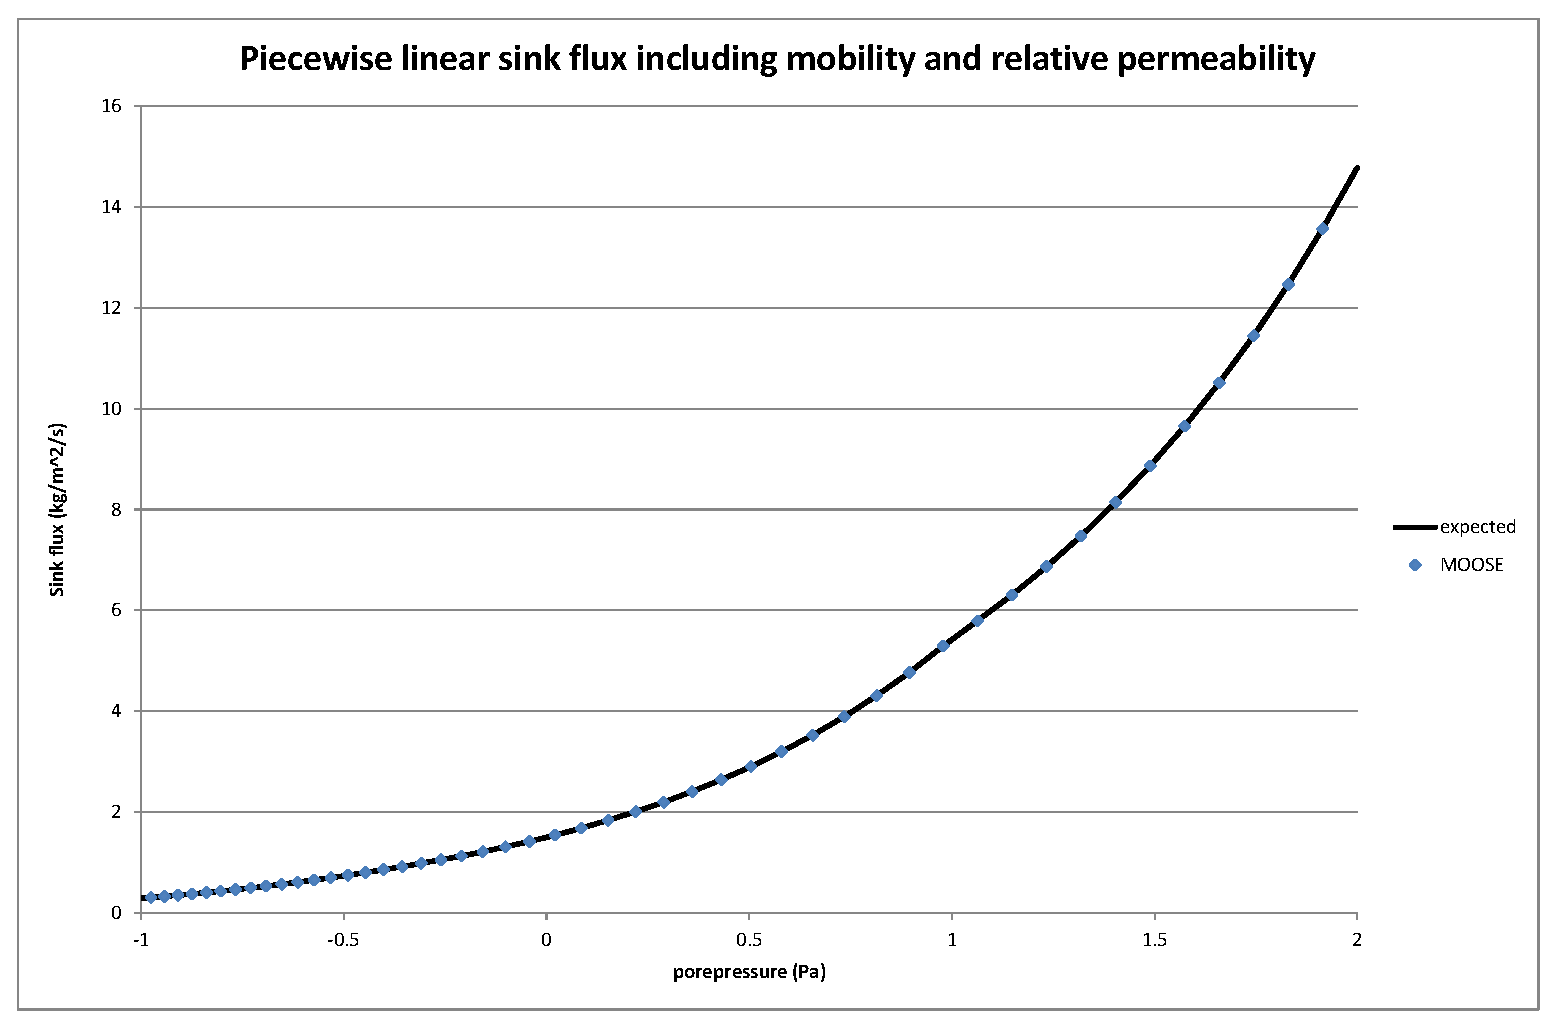
\includegraphics[width=7cm]{s03.eps} &
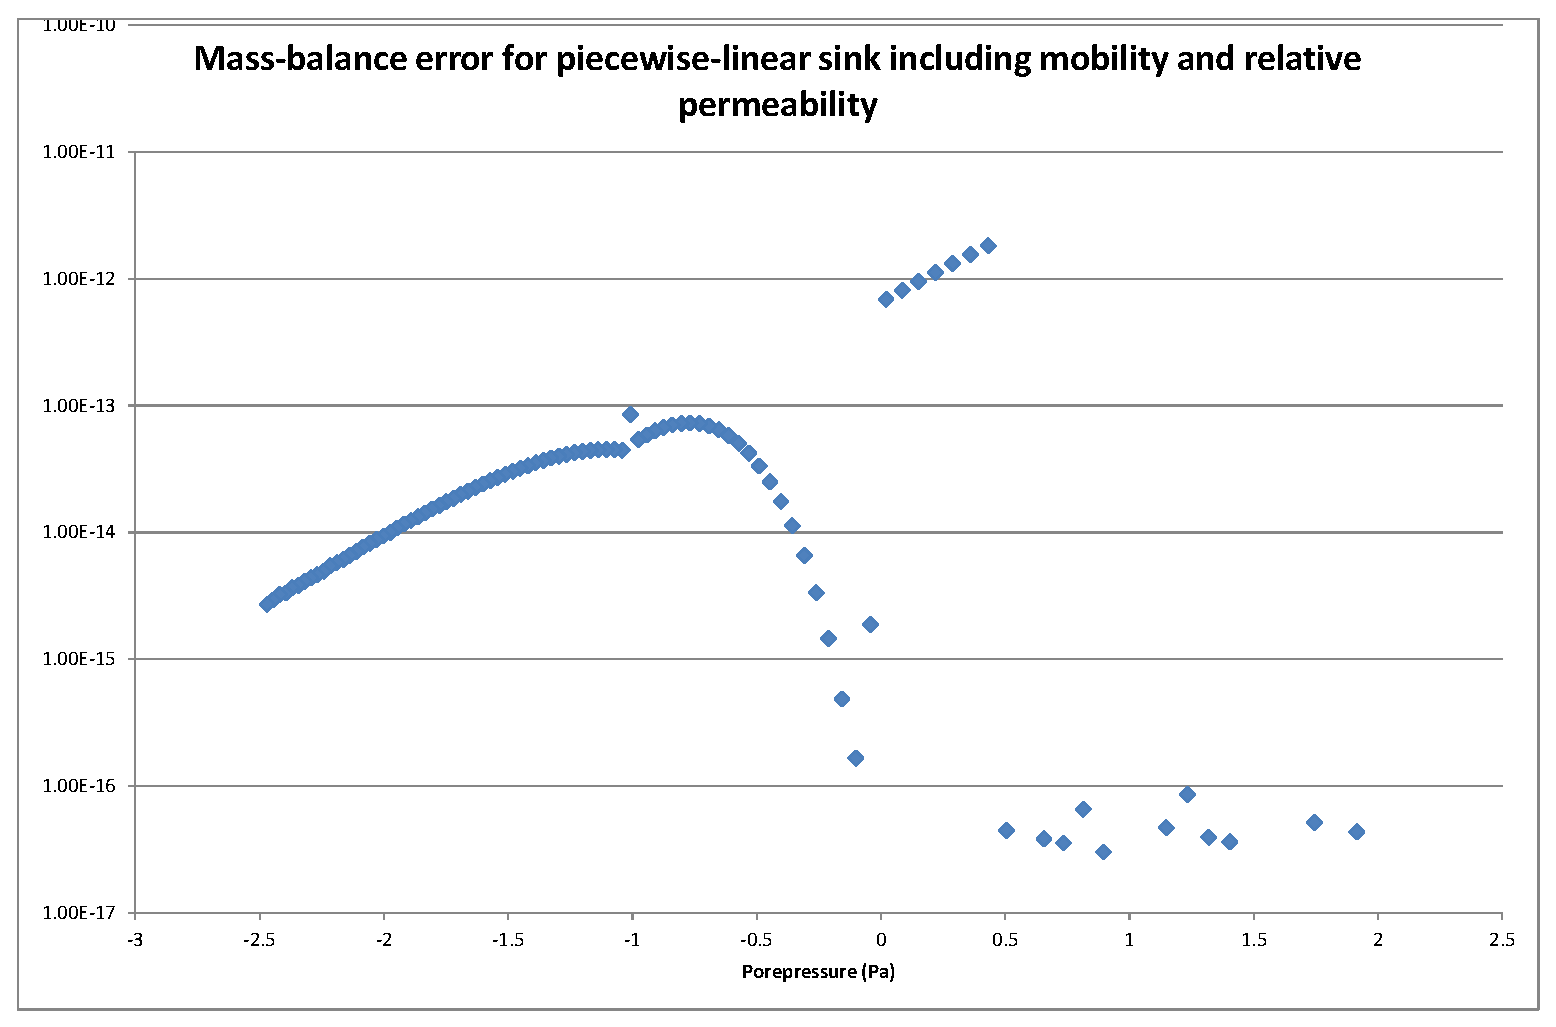
\includegraphics[width=7cm]{s03_mass_bal.eps}
\end{tabular}
\caption{Left: Comparison between the MOOSE result (in dots), and the
  expected behaviour of the sink flux given by Eqn~(\ref{eqn.s03}).
  Right: The mass-balance error is small for the simulation described
  demonstrating that the recorded sink flux is truly reducing the mass
  in the correct way.}
\label{s03.fig}
\end{figure}


\chapter{PolyLine sink}
\label{st}

The MOOSE implementation allows users to specify sinks and sources
acting along polylines that are functions of porepressure.  This is
primarily designed to model stream sources/sinks.  This chapter
tests that these sinks and sources act as specified.  The test is
part of the automatic test suite that is run every time the code is
updated.

A 3D model with $-1\leq x \leq 1$, $-1\leq y \leq 1$ and $-1\leq z
\leq 1$ with just a
single element is subjected to polyline sink flux acting at its
centre point.  Because it is a single element with the polyline
sitting at its centre, no fluid flow within the
element occurs.  The following fluid properties are used:
\begin{center}
\begin{tabular}{|ll|}
\hline
Constant fluid bulk modulus & 2\,GPa \\
Fluid density at zero pressure & 1000\,kg.m$^{-3}$ \\
\hline
\end{tabular} 
\end{center}
The test is fully-saturated, so the van Genuchten parameters, etc, are
irrelevant.  The initial porepressure is set to 10\,MPa, and the
polyline sink flux is applied with strength:
\begin{equation}
\mbox{sink flux (kg.s$^{-1}$)} = \left\{
\begin{array}{ll}
1 & \mbox{ for } p \leq 2\,\mbox{MPa} \\
1 + (p - 2)/6 & \mbox{ for } 2<p<8\,\mbox{MPa} \\
2 & \mbox{ for } p\geq 8\,\mbox{MPa}
\end{array}
\right.
\label{eqn.st01}
\end{equation}
The sink flux is recorded by into a Postprocessor by MOOSE.  It is
remotely possible that the MOOSE implementation {\em applies} the sink
flux incorrectly, but {\em records} it as a Postprocessor correctly as
specified by Eqn~(\ref{eqn.st01}).  Therefore the simulation also
records the fluid mass and mass-balance error in order to check that
the fluid mass is indeed being reduced correctly by the sink flux.
The simulation is run for 2.5\,s using 25 time steps.

The expected behaviour is demonstrated in Figure~\ref{st01.fig}.

\begin{figure}[htb]
\centering
\begin{tabular}{cc}
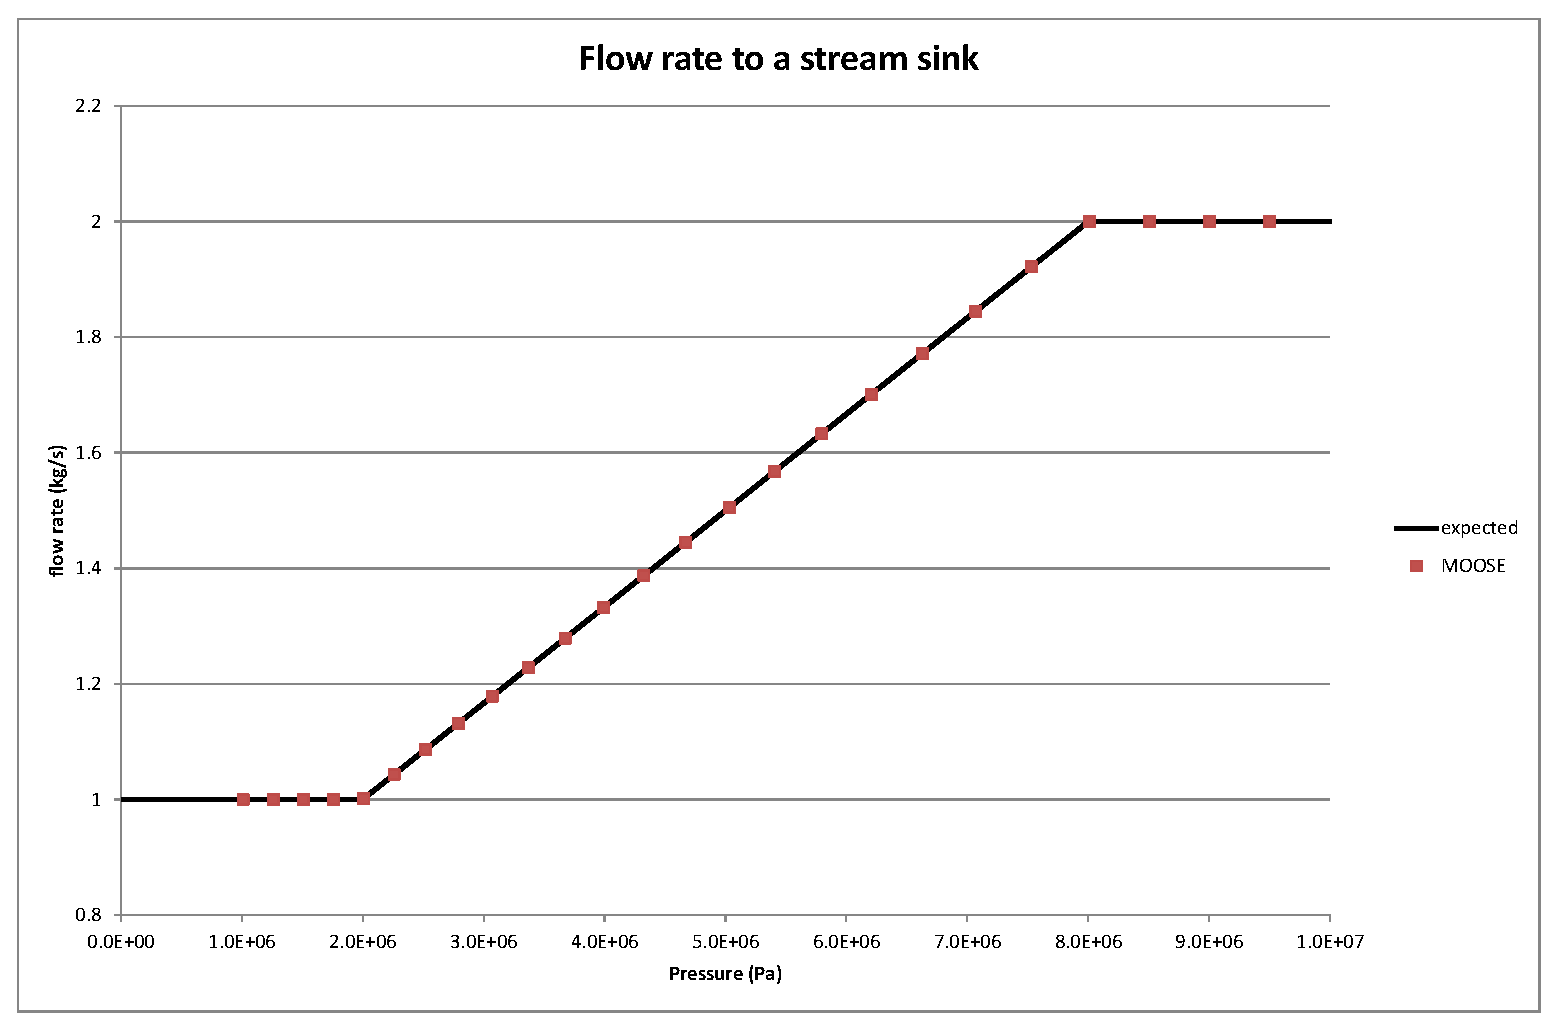
\includegraphics[width=7cm]{st01.eps} &
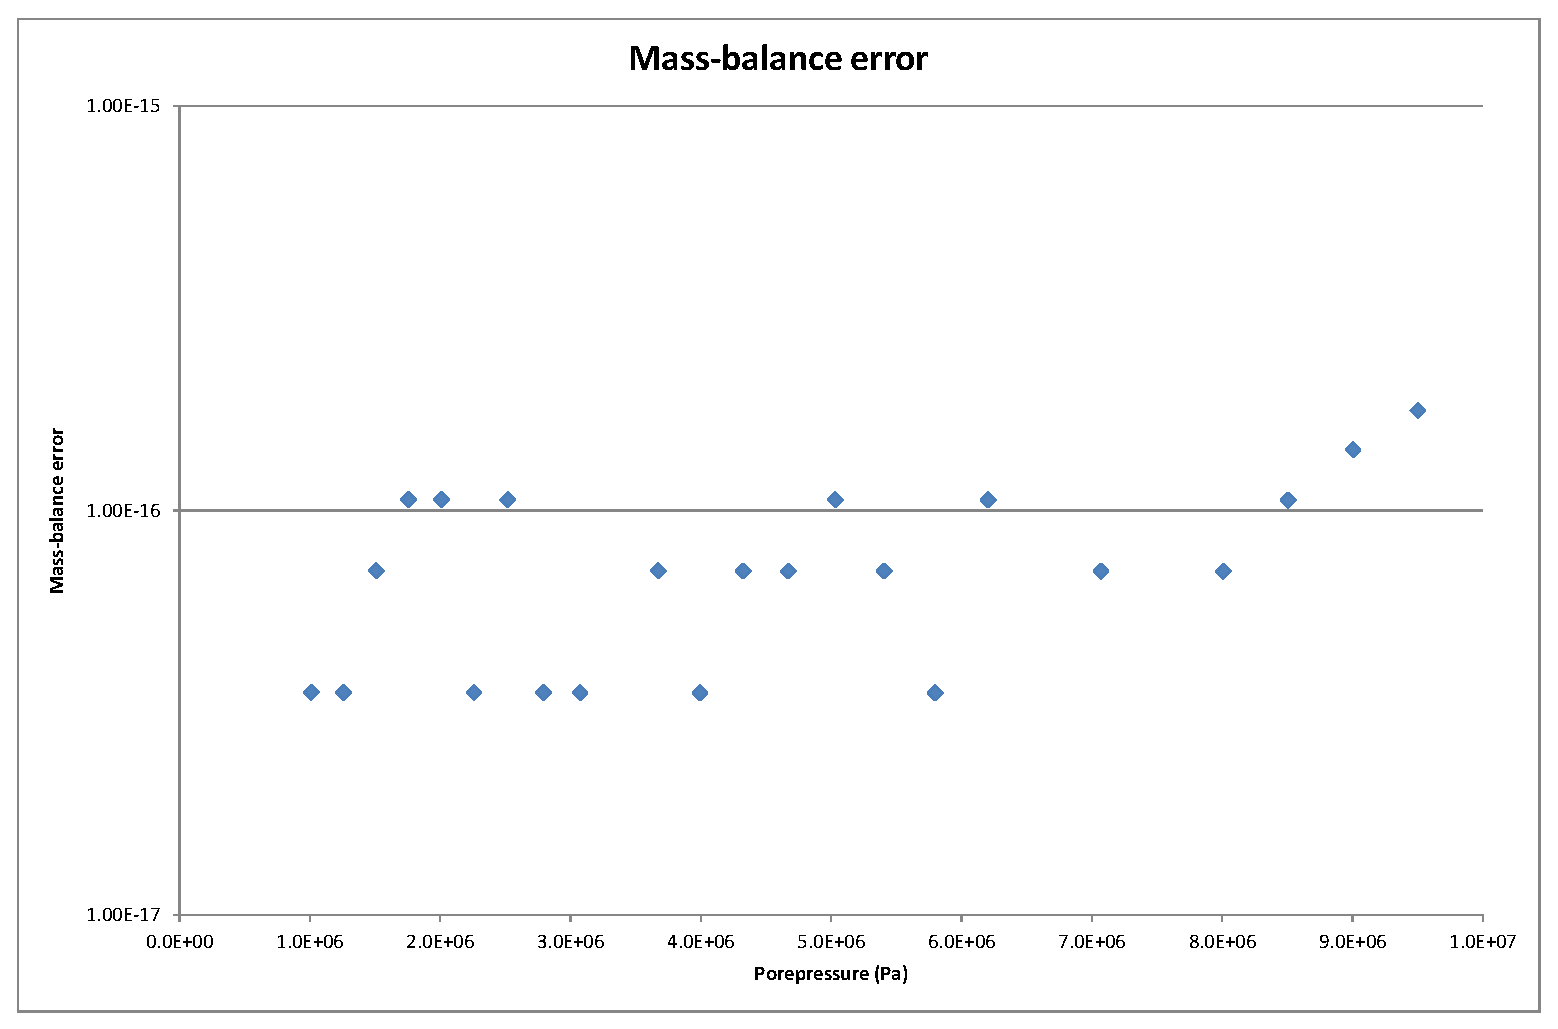
\includegraphics[width=7cm]{st01_mass_balance.eps}
\end{tabular}
\caption{Left: Comparison between the MOOSE result (in dots), and the
  expected behaviour of the sink flux given by Eqn~(\ref{eqn.st01}).
  Right: The mass-balance error is small for the simulation described
  demonstrating that the recorded sink flux is truly reducing the mass
  in the correct way.}
\label{st01.fig}
\end{figure}


\chapter{A pressure pulse in the fully saturated situation}
\label{pp}

Richards' equation for flow through a fully saturated medium without
gravity and without sources is just Darcy's equation
\begin{equation}
\frac{\partial}{\partial t}\phi\rho = \nabla_{i}\left(\frac{\rho
  \kappa_{ij}}{\mu} \nabla_{j}P \right) \ ,
\end{equation}
with notation described in the Theory Manual.  Using $\rho \propto
\exp(P/K)$, where $K$ is the fluid bulk modulus, Darcy's equation
becomes
\begin{equation}
\frac{\partial}{\partial t}\rho = \nabla_{i}\alpha_{ij}\nabla\rho \ ,
\end{equation}
with 
\begin{equation}
\alpha_{ij} = \frac{\kappa_{ij}B}{\mu\phi} \ .
\end{equation}
Here I've assumed the porosity and bulk modulus are constant in space
and time.

Consider the one-dimensional case were the spatial dimension is the
semi-infinite line $x\geq 0$.  Suppose that initially the pressure is
constant, so that
\begin{equation}
\rho(x, t=0) = \rho_{0} \ \ \ \mbox{for }\ \ x\geq 0 \ .
\end{equation}
Then apply a fixed-pressure Dirichlet boundary condition at $x=0$ so
that
\begin{equation}
\rho(x=0, t>0) = \rho_{\infty}
\end{equation}
The solution of the above differential equation is well known to be
\begin{equation}
\rho(x, t) = \rho_{\infty} + (\rho_{0} -
\rho_{\infty})\,\mbox{Erf}\left( \frac{x}{\sqrt{4\alpha t}} \right) \ ,
\label{eqn.exact.pp}
\end{equation}
where Erf is the error function.

This is verified by using the following six tests on a line of
10 elements.
\begin{enumerate}
\item Steady state 1-phase analysis to demonstrate that the
  steady-state of $\rho = \rho_{\infty}$ is achieved.
\item Transient 1-phase analysis with an unlumped time derivative.
\item Transient 1-phase analysis with a lumped time derivative.
\item Steady state 2-phase analysis with a fully-water saturated configuration.
\item Transient 2-phase analysis with unlumped time derivatives.
\item Transient 2-phase analysis with lumped time derivatives.
\end{enumerate}
An example verification is shown in Figure~\ref{pressure_pulse.fig}.
These tests run rapidly and are part of the automatic test suite.

\begin{figure}[htb]
\centering
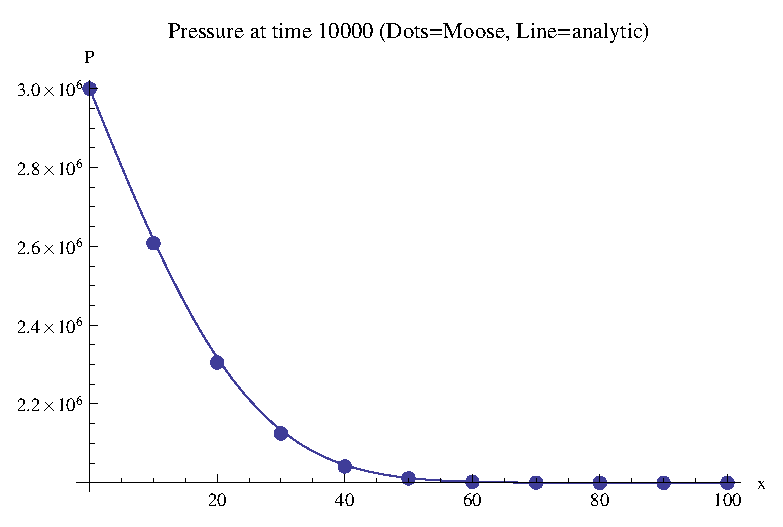
\includegraphics[width=10cm]{pressure_pulse.eps}
\caption{Comparison between the MOOSE result (in dots), and the
  exact analytic expression given by Eqn~(\ref{eqn.exact.pp}).  This
  test had 10 elements in the $x$ direction, with $0\leq x \leq
  100$\,m, and ran for a total of 
  10$^4$ seconds with 10 timesteps.  The parameters were $B=2$\,GPa,
  $\kappa_{xx}=10^{-15}$\,m$^{2}$, $\mu=10^{-3}$\,Pa.s, $\phi=0.1$,
  with initial pressure $P=2$\,MPa, and applied pressure $P=3$\,MPa at
  $x=0$.  For greater spatial resolution and smaller timesteps the
  agreement increases.  Both the single-phase simulation and the
  2-phase fully-water-saturated simulation give identical results for
  the water porepressure.}
\label{pressure_pulse.fig}
\end{figure}



\chapter{Newton cooling from a bar}
\label{nc}

This test demonstrates that MOOSE behaves correctly when a simulation
contains a sink.  The sink is a piecewise linear function of pressure.

Darcy's equation for flow through a fully saturated medium without
gravity and without sources is 
\begin{equation}
\frac{\partial}{\partial t}\phi\rho = \nabla_{i}\left(\frac{\rho
  \kappa_{ij}}{\mu} \nabla_{j}P \right) \ ,
\end{equation}
with notation described in the Theory Manual.  Using $\rho \propto
\exp(P/B)$, where $B$ is the fluid bulk modulus, Darcy's equation
becomes
\begin{equation}
\frac{\partial}{\partial t}\rho = \nabla_{i}\alpha_{ij}\nabla_{j}\rho \ ,
\end{equation}
with 
\begin{equation}
\alpha_{ij} = \frac{\kappa_{ij}B}{\mu\phi} \ .
\end{equation}
Here I've assumed the porosity and bulk modulus are constant in space
and time.

Consider the one-dimensional case where a bar sits between $x=0$ and
$x=L$ with initial pressure distribution so $\rho(x,t=0) = \rho_{0}(x)$.
Maintain the end $x=0$ at constant pressure, so that $\rho(x=0, t) =
\rho_{0}(0)$.  At the end $x=L$, prescribe a sink flux
\begin{equation}
\left.\frac{\partial\rho}{\partial x}\right|_{x=L} = -C\left(\rho -
\rho_{e}\right)_{x=L} \ ,
\end{equation}
where $\rho_{e}$ is a fixed quantity (``e'' stands for ``external''),
and $C$ is a constant conductance.  This corresponds to the flux
\begin{equation}
\left.\frac{\partial P}{\partial x}\right|_{x=L} = -CB\left(1 -
e^{(P_{e}-P)/B}\right)_{x=L} \ ,
\end{equation}
which can easily be coded into a MOOSE input file: the flux is
$\rho\kappa\nabla P/\mu = -CB\kappa(e^{P/B} - e^{P_{e}/B})/\mu$, and
this may be represented by a piecewise linear function of pressure.

The solution of this problem is well known and is
\begin{equation}
\rho(x, t) = \rho_{0}(0) - \frac{\rho_{0}(0) - \rho_{e}}{1 + LC}Cx +
\sum_{n=1}^{\infty} a_{n}\sin \frac{k_{n}x}{L}e^{-k_{n}^{2}\alpha
  t/L^{2}} \ ,
\end{equation}
where $k_{n}$ is the $n^{\mathrm{th}}$ positive root of the equation
$LC\tan k + k=0$  ($k_{n}$ is a little bigger than
$(2n-1)\pi/2$), and $a_{n}$ is determined from
\begin{equation}
a_{n}\int_{0}^{L}\sin^{2}\frac{k_{n}x}{L}\,\mathrm{d}x =
\int_{0}^{L}\left(\rho_{0}(x) - \rho_{0}(0) + \frac{\rho_{0}(0) -
  \rho_{e}}{1 + LC}Cx\right)\sin \frac{k_{n}x}{L}\,\mathrm{d}x \ ,
\end{equation}
which may be solved numerically (I have used Mathematica to generate
the solution in Figure~\ref{nc.fig}).

\noindent The problem is solved in MOOSE using the following parameters:
\begin{center}
\begin{tabular}{|ll|}
\hline
Bar length & 100\,m \\
Bar porosity & 0.1 \\
Bar permeability & $10^{-15}$\,m$^{2}$ \\
\hline
Gravity & 0 \\
\hline
Water density & 1000\,kg.m$^{-3}$ \\
Water viscosity & 0.001\,Pa.s \\
Water bulk modulus & 1\,MPa \\
\hline
Initial porepressure $P_{0}$ & 2\,MPa \\
Environmental pressure $P_{e}$ & 0 \\
\hline
Conductance $C$ & 0.05389\,m$^{-1}$ \\
\hline
\end{tabular} \\
\end{center}
This conductance is chosen so at steadystate $\rho(x=L)=2000$\,kg.m$^{-3}$.

The problem is solved using 1000 elements along the $x$ direction
($L=100$\,m), and using 100 time-steps of size $10^6$\,s.  Using fewer
elements or fewer timesteps means the agreement with the theory is
marginally poorer.  Two tests are performed: one with a lumped time
derivative and one with an unlumped derivative, giving almost
indistinguishable results.  The problem is also
solved using the steadystate solver.  In this case the initial
condition is $P=2-x/L$\,MPa, since the uniform $P=2$\,MPa does not
converge.  The results are shown in Figure~\ref{nc.fig}.

\begin{figure}[htb]
\begin{center}
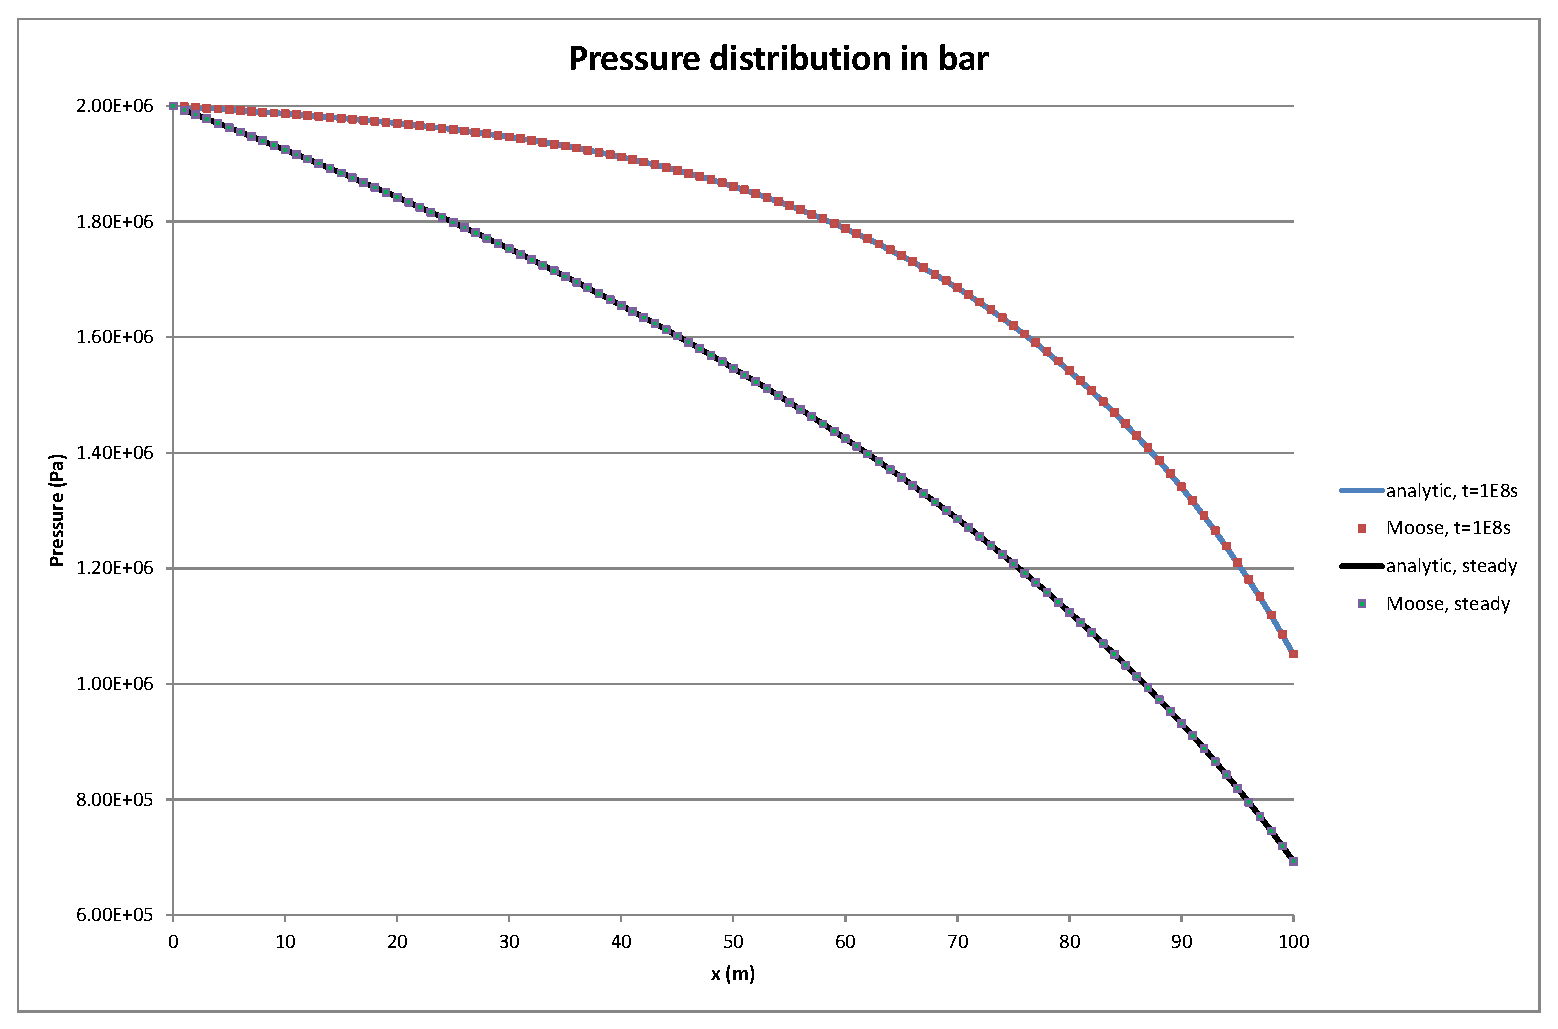
\includegraphics[width=17cm]{nc.eps}
\caption{The porepressure in the bar at $t=10^{8}$\,s, and at
  steadystate.  The pressure at $x=0$ is held fixed, while the sink is
  applied at $x=100$\,m.  MOOSE agrees well with theory demonstrating
  that piecewise-linear sinks/sources are correctly implemented in MOOSE.}
\label{nc.fig}
\end{center}
\end{figure}


\chapter{The Theis problem}
\label{th}

The Theis problem is related to an aquifer pumping test where water is
withdrawn at a constant rate, $Q$ (m$^{3}$.s$^{-1}$) from an
isotropic, infinite, fully-saturated, confined aquifer.  Water is withdrawn
using a vertical borehole of negligible radius that spans the entire
aquifer height, $b$ (m).  In the Theis solution, gravitational
effects are ignored (the pressures at the bottom and top of the
aquifer are is assumed equal).  At some horizontal radial distance, $r$, from
the borehole the pressure is measured.  The geometry is shown in
Figure~\ref{th.setup.fig}. 

\begin{figure}[htb]
\begin{center}
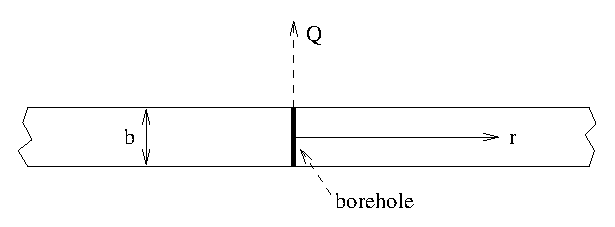
\includegraphics[width=8cm]{th.setup.eps}
\caption{The Theis problem: An isotropic infinite, fully-saturated,
  confined aquifer of vertical height $b$ is subjected to pumping at
  rate $Q$ via a vertical borehole that spans the entire height of the
  aquifer.  The pressure is measured at a radial distance $r$.}
\label{th.setup.fig}
\end{center}
\end{figure}

\section{Derivation of the Theis solution}

Theis solved this problem\footnote{CV Theis, ``The relation between
  the lowering of the piezometric surface and the rate and duration of
  discharge of a well using groundwater storage''.  Transactions,
  American Geophysical Union 16 (1935) 519--524}, and the derivation
is given now using the Theory Manual notation.  Darcy's equation reads
\begin{equation}
\phi \frac{\partial}{\partial t} \rho S = \nabla\cdot \left(\frac{\rho
  \kappa}{\mu} (\nabla P - \rho {\mathbf{g}}) \right) \ ,
\end{equation}
where $\phi$ is the aquifer porosity, $t$ is time, $\rho$ is the water
density, $S$ is the water saturation, $\nabla$ is the spatial
derivative, $\kappa$ is the isotropic permeability, $\mu$ is the water
viscosity, and $P$ is the water pressure.  Assume the following
\begin{itemize}
\item The problem is fully saturated, $S=1$, and gravitational
  effects are ignored, ${\mathbf{g}} = {\mathbf{0}}$.
\item The bulk modulus, $K_{\mathrm{w}}$, of water is constant so that
  $\rho = \rho_{0}e^{P/K_{\mathrm{w}}}$.
\item The problem studied has the property
\begin{equation}
\left| \nabla^{2}P \right| \gg \left|\frac{(\nabla
  P)^{2}}{K_{\mathrm{w}}} \right|  \ .
\label{assumption.eqn}
\end{equation}
This inequality will be explored below.
\end{itemize}
\noindent Under these assumptions, Darcy's equation reads
\begin{equation}
\frac{\phi}{K_{\mathrm{w}}} \frac{\partial}{\partial t}P =
\frac{K}{\mu}\nabla^{2}P \ ,
\end{equation}
which, in this 2D case, has the standard exponential integral solution
\begin{equation}
P(r,t) = P_{0} - \alpha \int_{\frac{r^{2}\phi\mu}{4 t \kappa
    K_{\mathrm{w}}}}^{\infty} \frac{1}{u} e^{-u}\,\mathrm{d} u \ .
\end{equation}
Applying the boundary condition at $r=0$ that the rate of change of
volume of water in the aquifer is $Q$ yields the coefficient $\alpha$,
and the solution becomes
\begin{equation}
P(r,t) = P_{0} - \frac{Q\mu}{4\pi b \kappa} \int_{\frac{r^{2}\phi\mu}{4 t \kappa
    K_{\mathrm{w}}}}^{\infty} \frac{1}{u} e^{-u}\,\mathrm{d} u \ .
\label{eqn.theis}
\end{equation}

\section{Transmissivity, Storativity and Well function}

The hydrogeology literature uses different notation.  It defines the
head, $h=P/\rho g$; the transmissivity, $T = \kappa\rho g b/\mu$; the
storativity, $S = b\rho 
g \phi/K_{\mathrm{w}}$; and the well function $W(x) =
\int_{x}^{\infty}u^{-1}e^{-u}\mathrm{d}u$, so that the Theis solution,
Eqn~(\ref{eqn.theis}) becomes
\begin{equation}
h(r,t) = h_{0} - \frac{Q}{4\pi T} W
\left(\frac{r^{2}S}{4Tt} \right) \ .
\end{equation}

\section{Comparison with MOOSE}

A Moose model defined by a cylinder of radius 3\,km with 1500
hexahedral elements is created.  The plan mesh is shown in
Figure~\ref{th.mesh.fig}.  The well is situated at $r=0$, and the
pressure is measured at $r=50$\,m.  The pumping is modelled using a
PolyLineSink with constant rate.

\begin{figure}[htb]
\begin{center}
\begin{tabular}{cc}
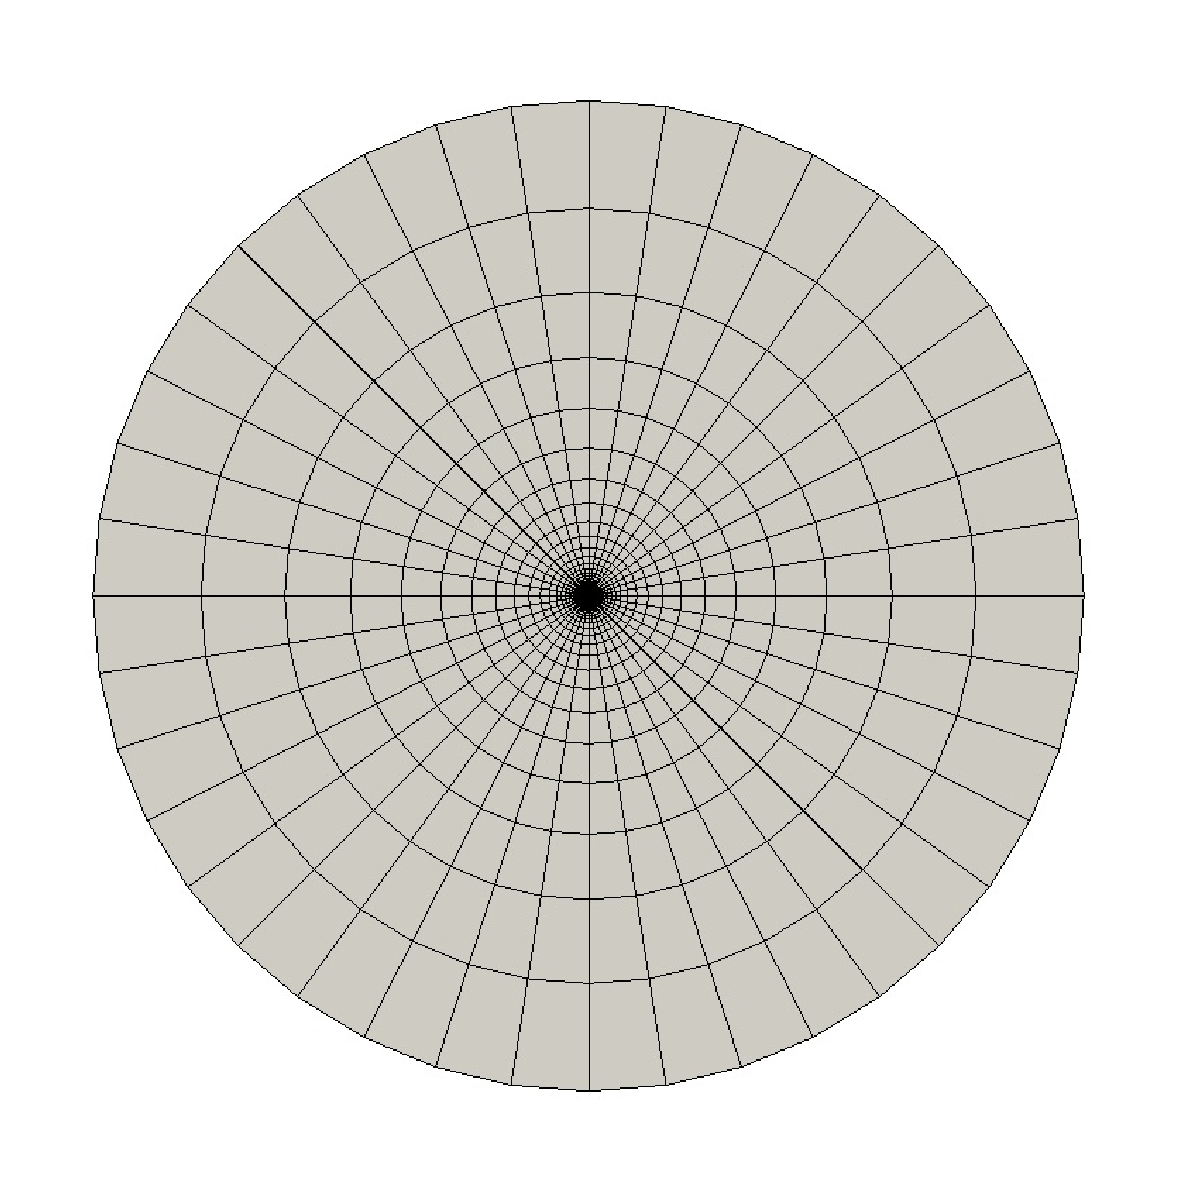
\includegraphics[width=6cm]{th_mesh.eps} &
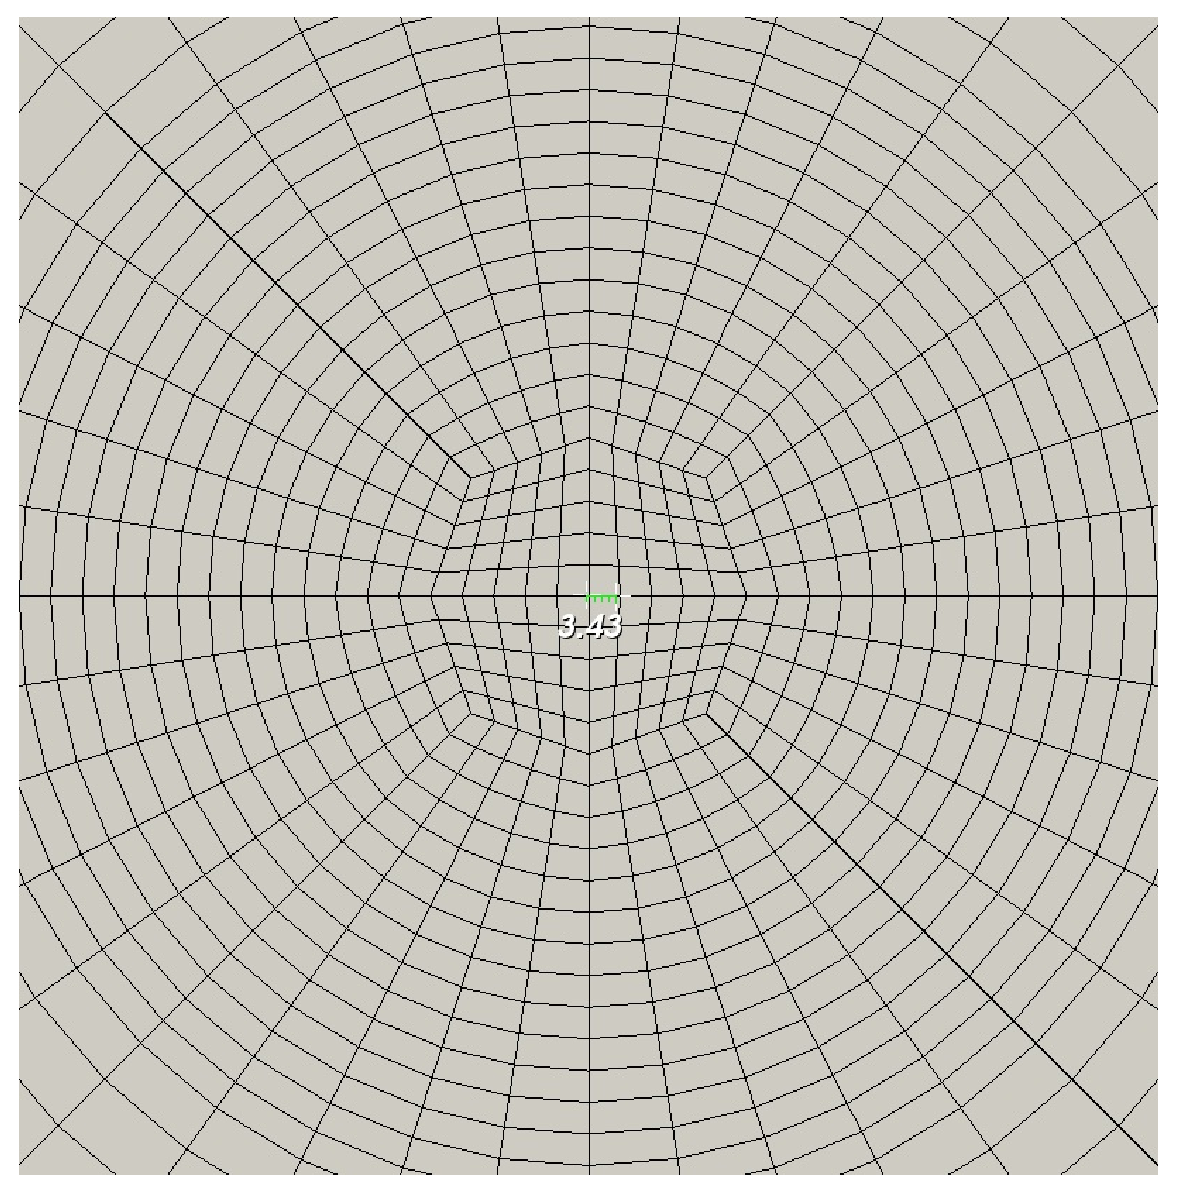
\includegraphics[width=6cm]{th_mesh_zoom.eps}
\end{tabular}
\caption{The mesh for the Theis problem has 1500 elements, and a
  radius of 3\,km.  Left: the whole plan mesh.  Right: the region
  $r\leq 50$\,m.}
\label{th.mesh.fig}
\end{center}
\end{figure}

The following parameters are used:
\begin{center}
\begin{tabular}{|ll|}
\hline
Aquifer porosity, $\phi$ & 0.1 \\
Aquifer permeability, $\kappa$ & $10^{-10}$\,m$^{2}$ \\
\hline
Water viscosity, $\mu$ & 0.001\,Pa.s \\
Water bulk modulus, $K_{\mathrm{w}}$ & 2\,GPa \\
\hline
Gravity & 0.0 \\
Aquifer thickness, $b$ & 20\,m  \\
Pumping rate, $Q$ & 0.2\,m$^{3}$.s$^{-1}$ \\
\hline
\end{tabular}
\end{center}
The van-Genuchten parameters, etc, are unimportant as this is a
fully-saturated simulation.

Eqn~(\ref{assumption.eqn}) contains an important assumption of the
Theis solution which constrains the validity of the result.
Substituting the solution, Eqn~(\ref{eqn.theis}), into the assumption
yields
\begin{equation} 
\frac{1}{u} e^{-u} \ll \frac{4 \pi b \kappa K_{\mathrm{w}}}{Q\phi\mu}
= \frac{4\pi b T}{QS} \ ,
\end{equation}
where
\begin{equation}
u = \frac{r^{2}\phi\mu}{4t\kappa K_{\mathrm{w}}} = \frac{r^{2}S}{4tT}
\ .
\end{equation}
In the situation under study, substituting the numerical values given
above yields $u^{-1}e^{-u} \ll 2.5\times 10^{6}$, or $u\gg 4\times
10^{-7}$.  When $r=50$\,m, this yields $t\ll 8\times 10^{5}$\,s.

Figure~\ref{th01.fig} shows good agreement between the Theis solution
and the MOOSE implementation.  Both 1-phase and fully-water-saturated
2-phase models give the same result, both with and without
time-derivative lumping.  These four tests are not part of the
automatic test suite since they take around 20\,seconds to complete.
They are therefore marked as ``heavy'' and is not run every time the
code is updated.  However, four similar tests (both 1-phase and
fully-water-saturated 2-phase, both with and without mass lumping) on
a coarser mesh with only 272 elements, that also take larger
timesteps, give similar drawdowns (to within 0.1\,m), and are part of
the automatic test suite.

\begin{figure}[htb]
\centering
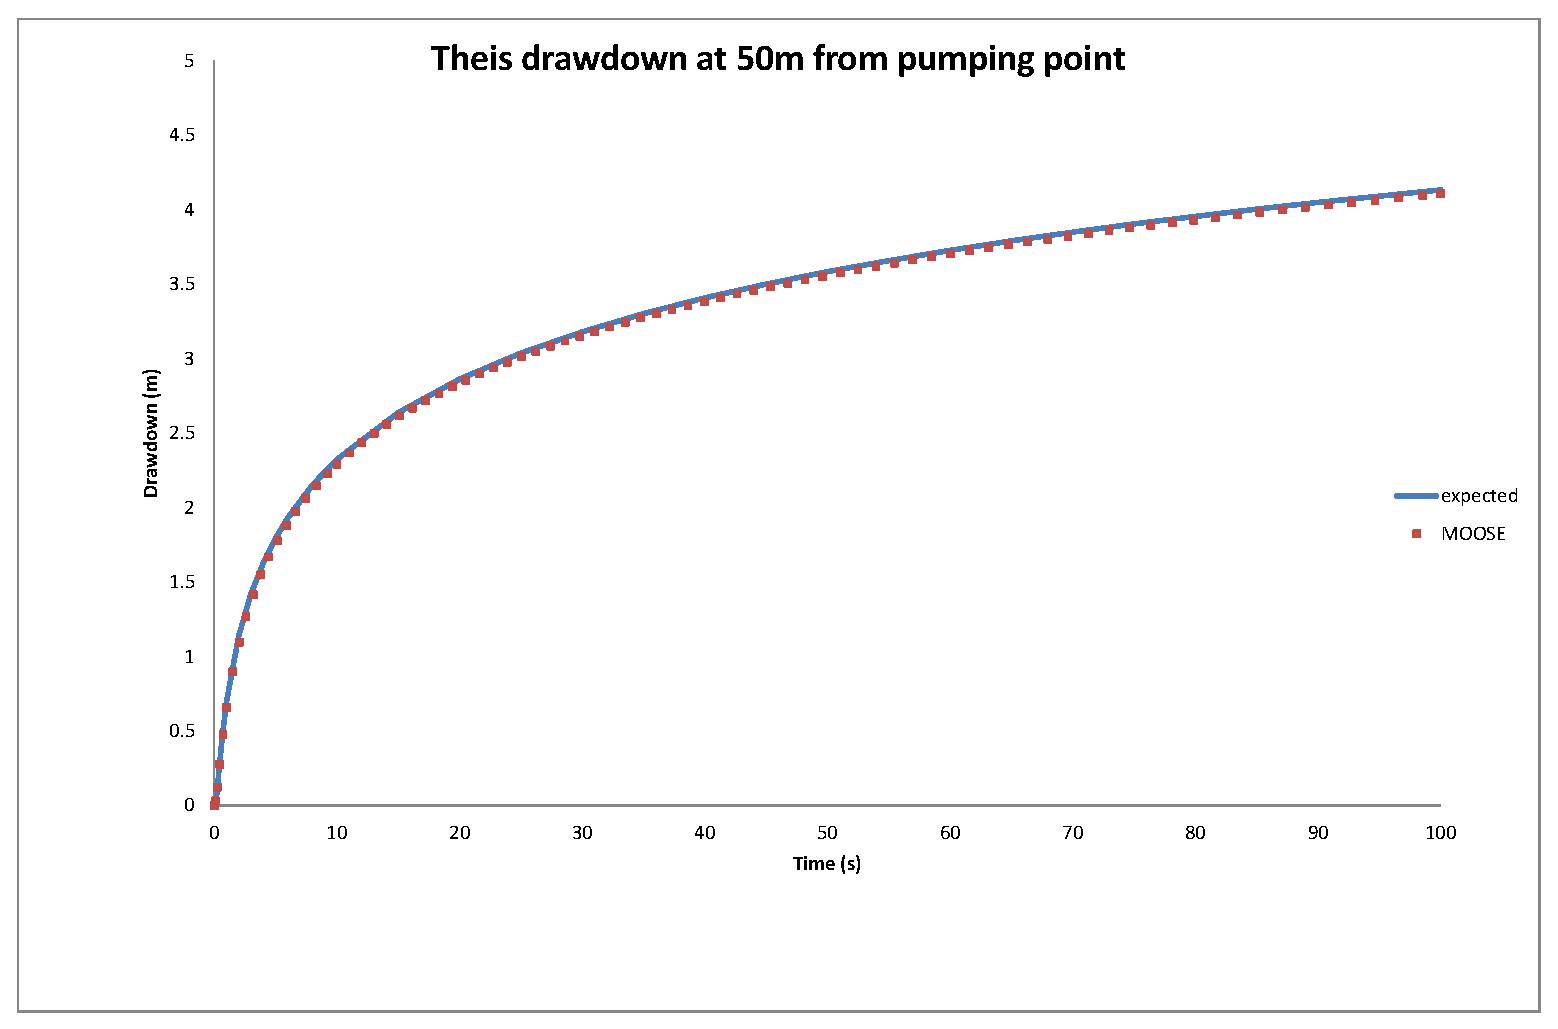
\includegraphics[width=14cm]{th01.eps}
\caption{Comparison between the MOOSE result (in dots: both 1-phase
  and 2-phase fully-saturated, both with and without mass lumping give
  indistinguishable results and the
  expected behaviour of the drawdown as given by Eqn~(\ref{eqn.theis})
  (drawdown is $P/\rho g$, or $P/10000$ in this model).}
\label{th01.fig}
\end{figure}


\chapter{Boreholes}
\label{bh}

As detailed in the Theory Manual, a borehole defined by a curve (or,
most often, a straight line segment) in 3D space is modelled by a
sequence of Dirac points.  At each point, a flux is prescribed:
\begin{equation}
f = W|C(P-P_{\mathrm{bh}})| \frac{\rho \kappa_{\mathrm{rel}}}{\mu} (P - P_{\mathrm{bh}}) \ ,
\label{bh.propto.eqn}
\end{equation}
where $P$ is the porepressure at the Dirac point, and
$P_{\mathrm{bh}}$ is the borehole pressure at that point (an input
parameter).  The other parameters are: $C$, the character of the
borehole (eg, ``production'' has $C=1$ for $P>P_{\mathrm{bh}}$ and zero
otherwise); $\rho$ is the fluid density; $\kappa_{\mathrm{rel}}$ is
the relative permeability; and $\mu$ is the fluid viscosity.   The
coefficient of proportionality,, $W$ in this expression is a
complicated function of the geometry of the finite element (or the
neighbouring elements if the Dirac point is on an elemental boundary)
and the rock permeability, and the borehole radius at that point.

\section{Rotation matrices}
The well constant $W$ in Eqn~(\ref{bh.propto.eqn})
involves the rotation matrices that transforms between Cartesian
$(x,y,z)$ coordinates and coordinates in which the $z$ axis lies along
the local direction of the borehole.
\begin{itemize}
\item The first borehole test checks that these rotation matrices are
  formed correctly for random alignments of boreholes.
\end{itemize}
This test is very fast to run (it does not involve any fluid flow) and
is part of the automatic test suite.

\section{Fluxes}
The automatic test suite also contains four tests that check that
Eqn~(\ref{bh.propto.eqn}) is correctly implemented for given $W$ (the
Peaceman formulation is used) by placing a vertical borehole through
the centre of a single element, and measuring the fluid flow to the
borehole as a function of porepressure $P$.  These four tests are:
\begin{itemize}
\item A production borehole with $P_{\mathrm{bh}} = 0$, with a
  fully-saturated medium
\item An injection borehole with $P_{\mathrm{bh}} = 10$\,MPa, with a
  fully-saturated medium
\item A production borehole with $P_{\mathrm{bh}} = -1$\,MPa, with an
  unsaturated medium
\item An injection borehole with $P_{\mathrm{bh}} = 0$, with an
  unsaturated medium
\end{itemize}
The parameters common to these four tests are:
\begin{center}
\begin{tabular}{|ll|}
\hline
Element size & $2\times 2\times 2$\,m$^{3}$ \\
Borehole radius & 0.1\,m \\
Bar permeability & $10^{-12}$\,m$^{2}$ \\
Gravity & 0 \\
Unit fluid weight & 0 \\
Fluid reference density & 1000\,kg.m$^{-3}$ \\
Fluid bulk modulus & 2\,GPa \\
Fluid viscosity & $10^{-3}$\,Pa.s \\
Van Genuchten $\alpha$ & $10^{-5}$\,Pa \\
Van Genuchten $m$ & 0.8  \\
Immobile saturation & 0 \\
Relative permeability $n$ & 2 \\
\hline
\end{tabular} \\
\end{center}
It is remotely possible that the MOOSE implementation {\em applies}
the borehole flux incorrectly, but {\em records} it as a Postprocessor
correct as specified by Eqn~(\ref{bh.propto.eqn}).  Therefore, these
four simulations also record the fluid mass and mass-balance error in
order to check that the fluid mass is indeed being correctly changed
by the borehole.  Figure~\ref{bh02_05.fig} demonstrates that
Eqn~(\ref{bh.propto.eqn}) is indeed correctly implemented in MOOSE.

\begin{figure}[htb]
\centering
\begin{tabular}{cc}
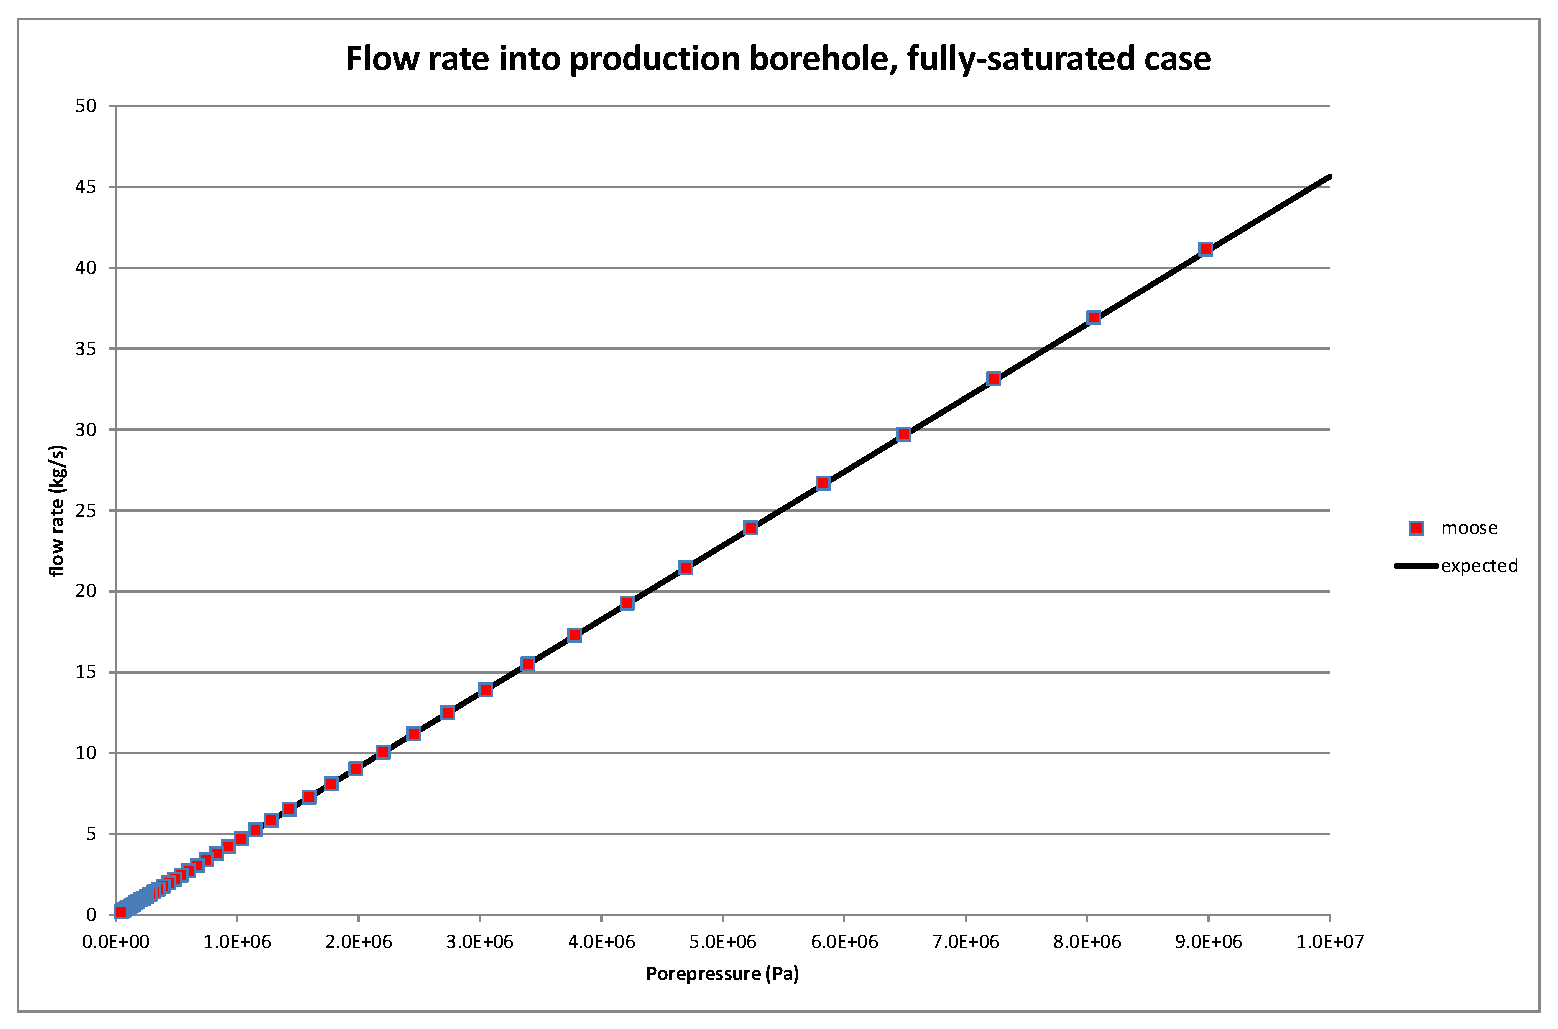
\includegraphics[width=7cm]{bh02.eps} &
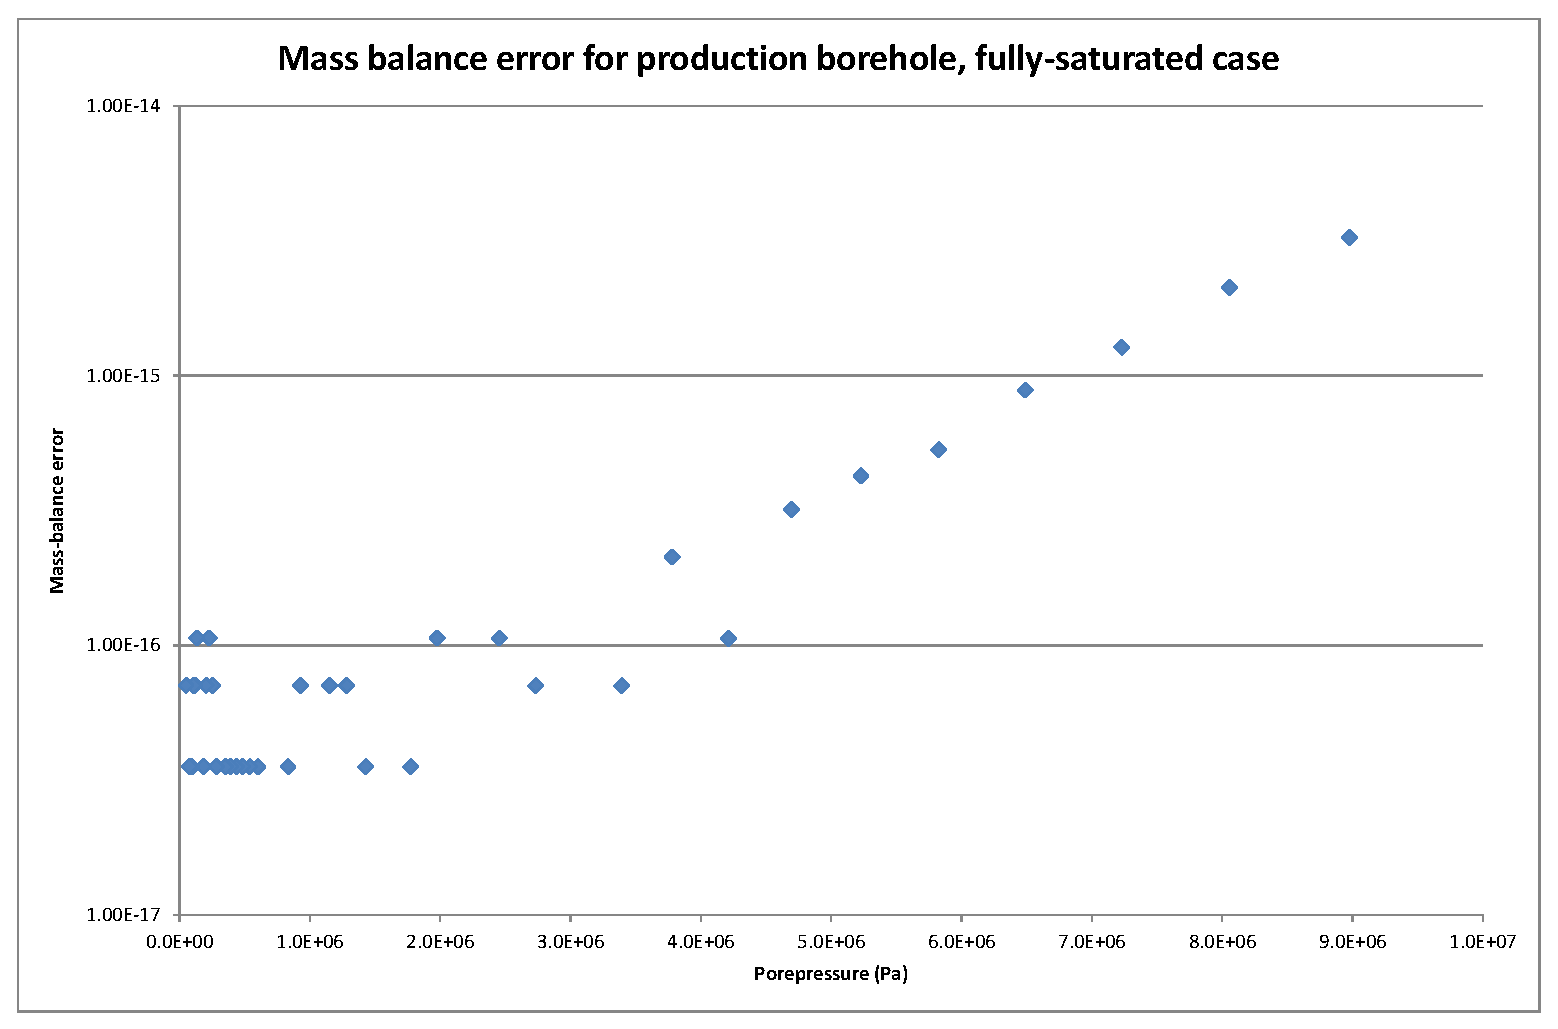
\includegraphics[width=7cm]{bh02_mass_balance.eps} \\
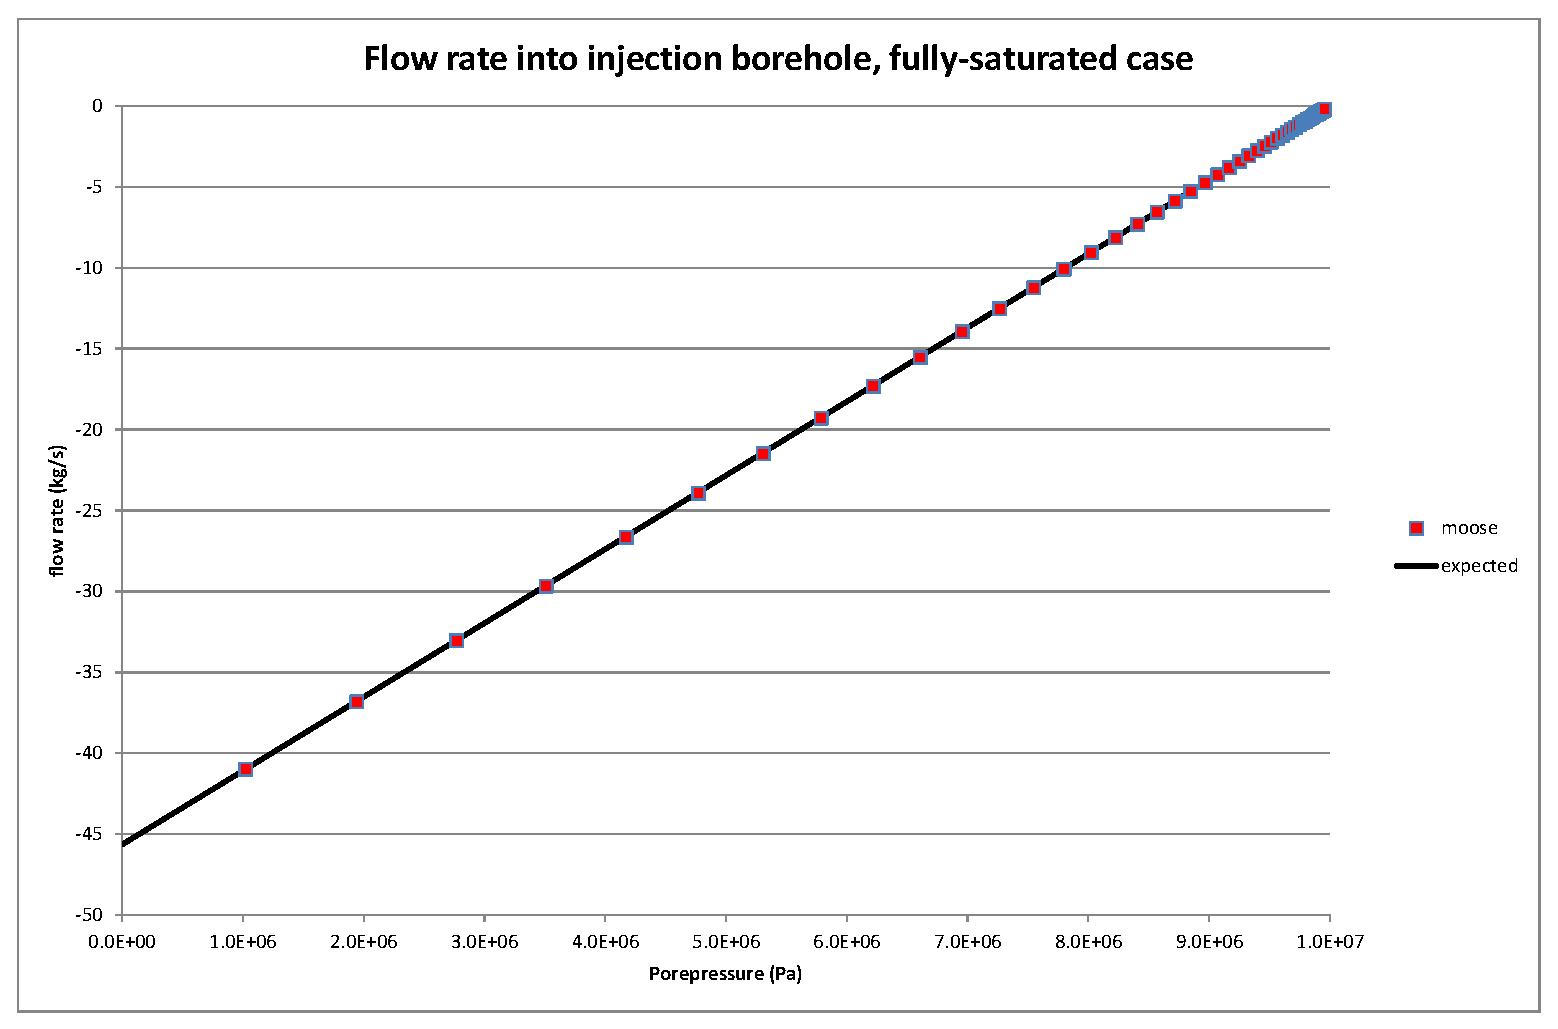
\includegraphics[width=7cm]{bh03.eps} &
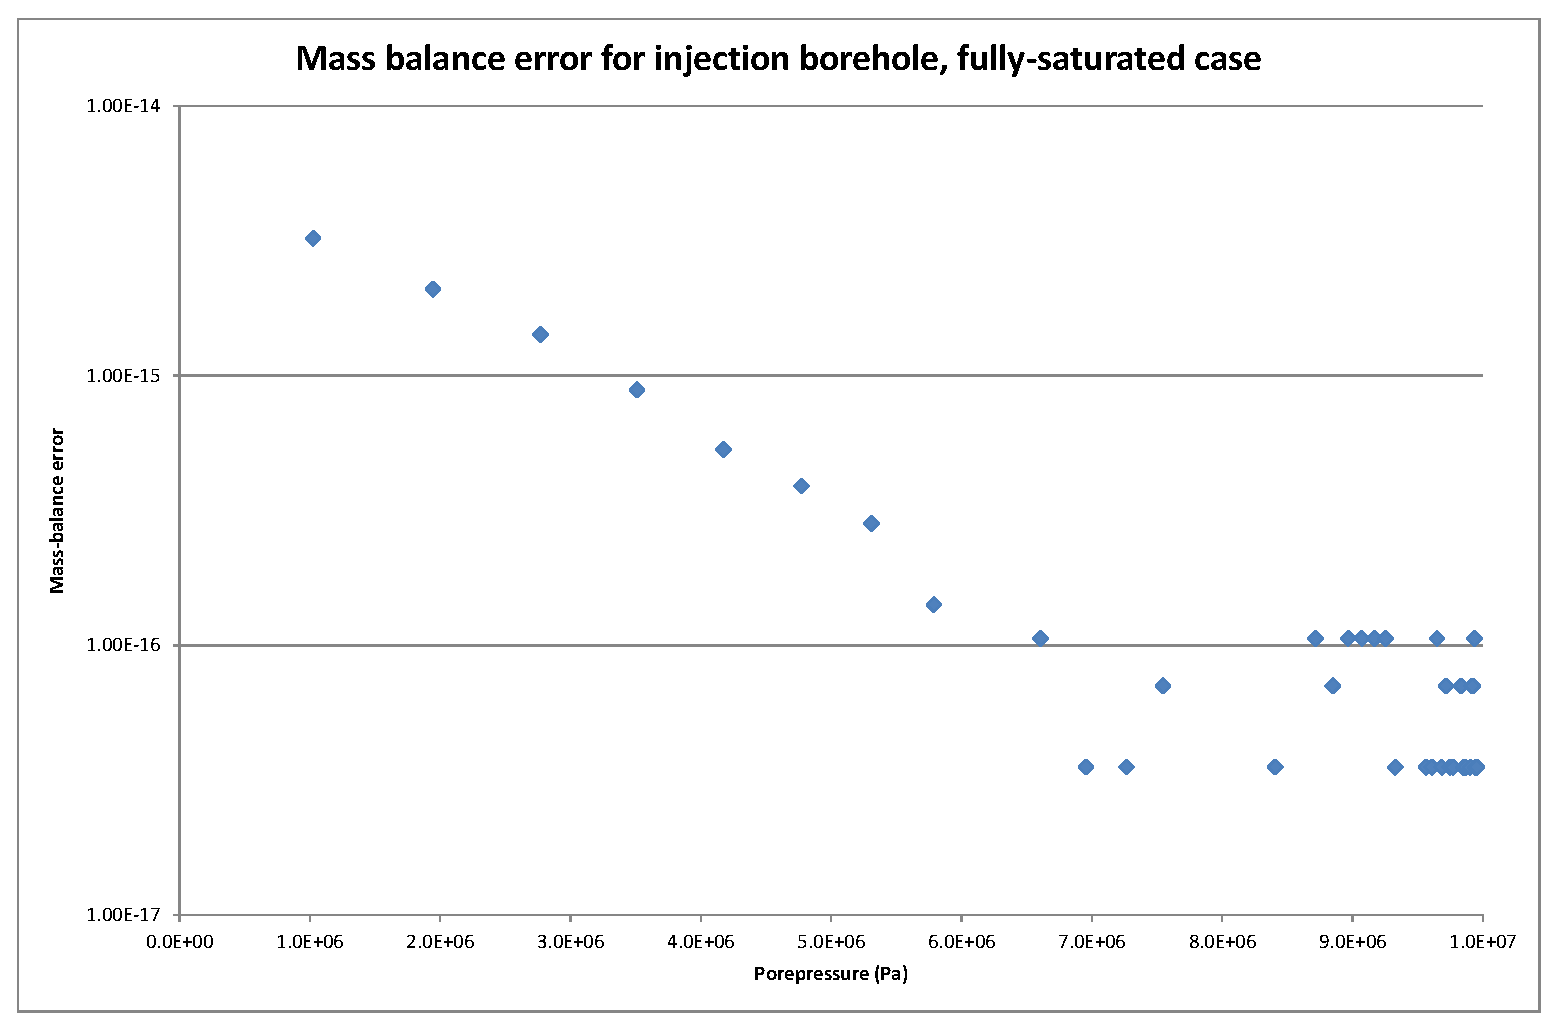
\includegraphics[width=7cm]{bh03_mass_balance.eps} \\
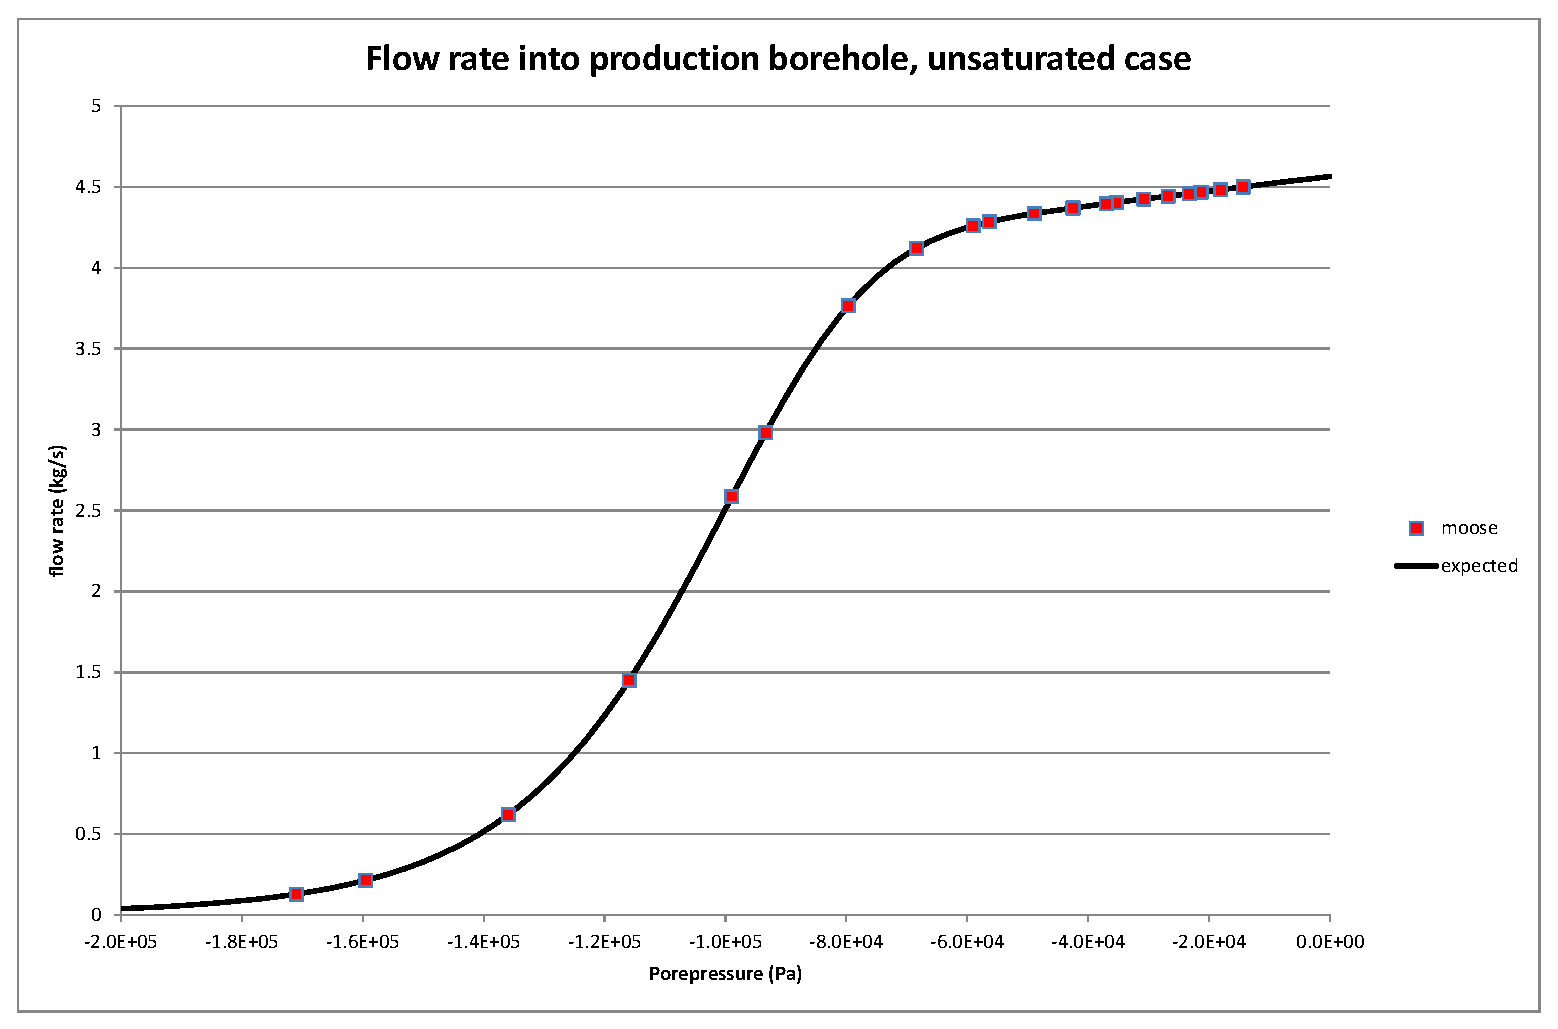
\includegraphics[width=7cm]{bh04.eps} &
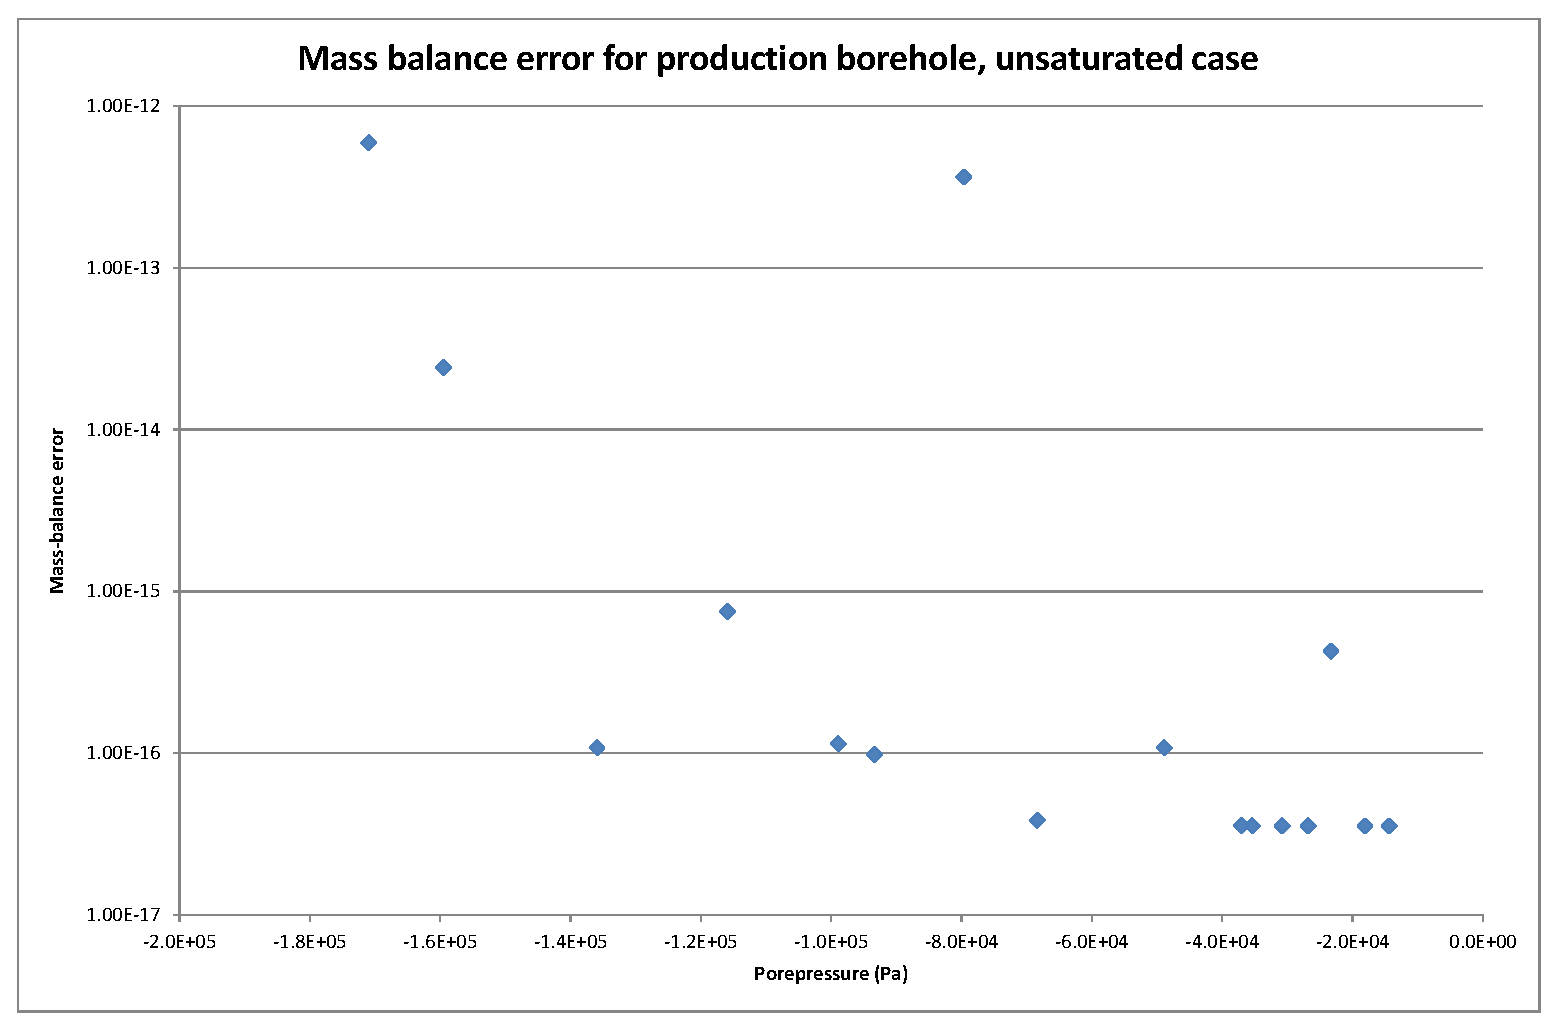
\includegraphics[width=7cm]{bh04_mass_balance.eps} \\
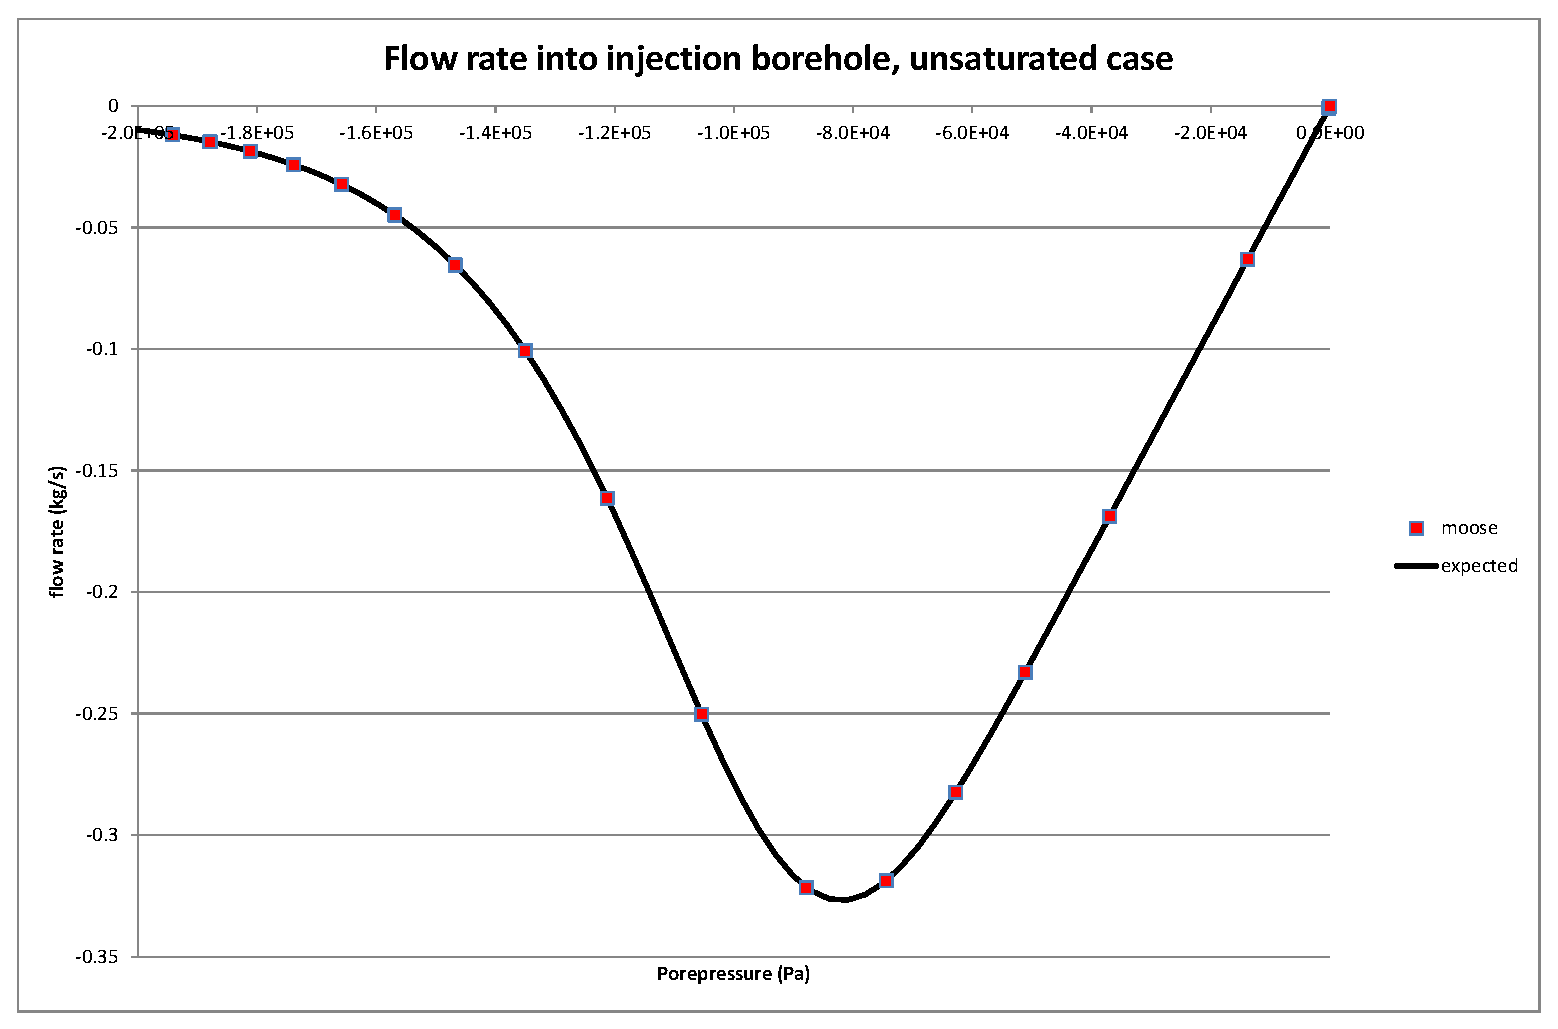
\includegraphics[width=7cm]{bh05.eps} &
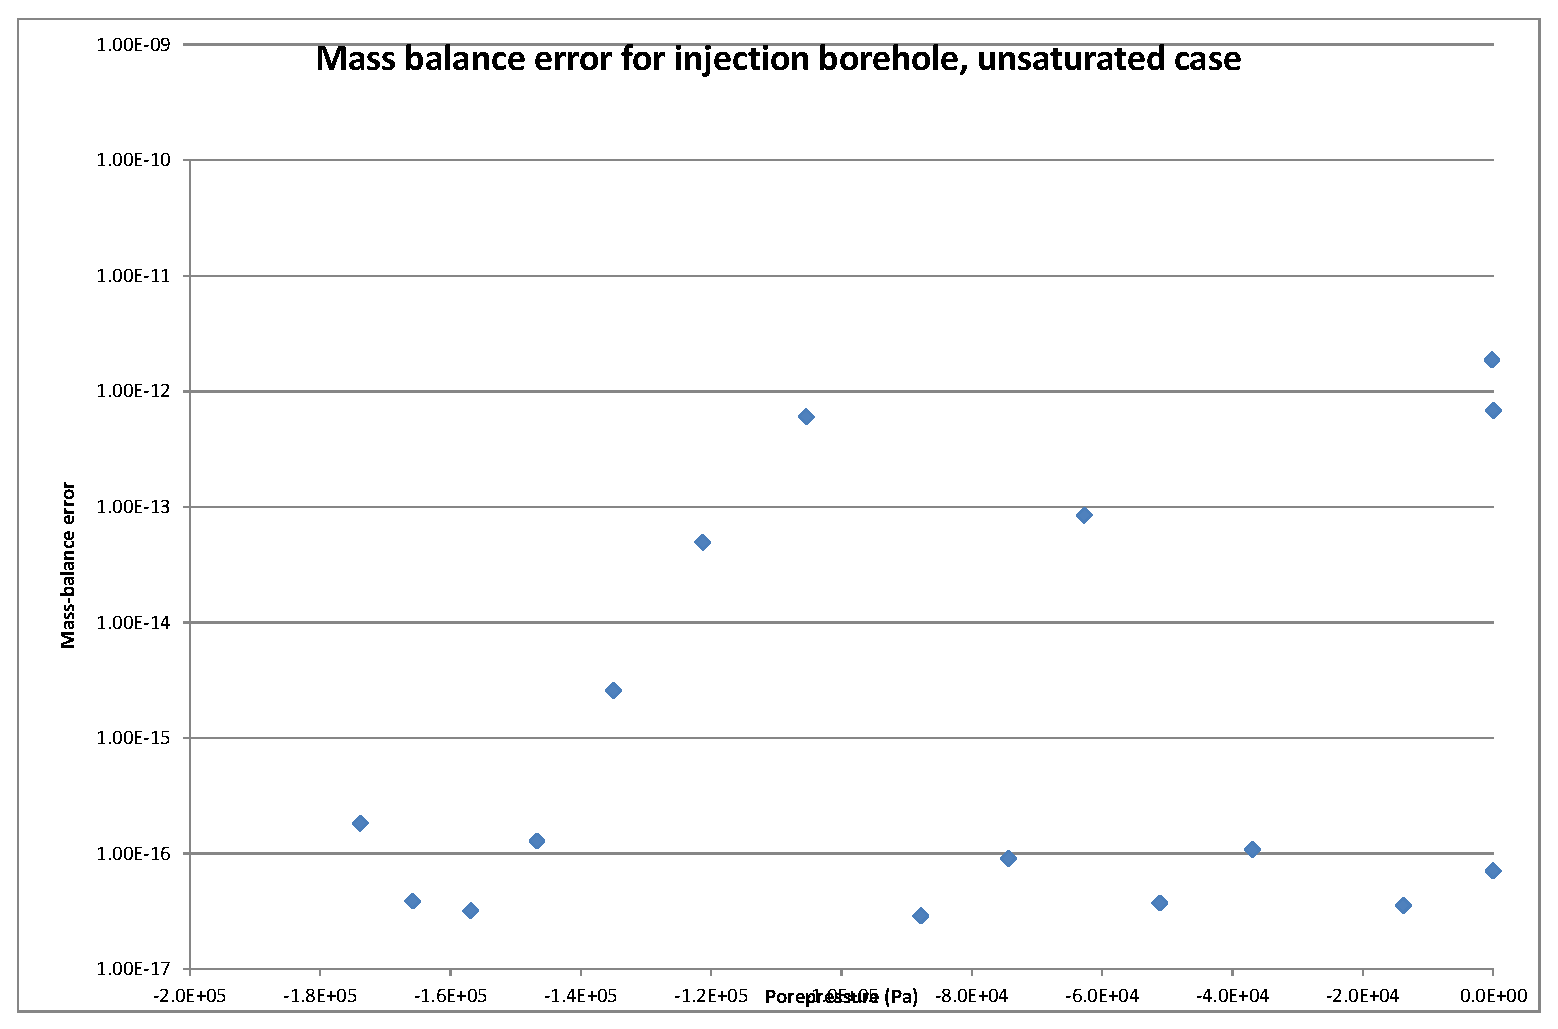
\includegraphics[width=7cm]{bh05_mass_balance.eps}
\end{tabular}
\caption{Left figures: Comparison between the MOOSE result (in dots), and the
  expected behaviour of the borehole flux given by
  Eqn~(\ref{bh.propto.eqn}) (as a line) for the cases listed in the text.  Right
  figures: The mass balances, which are all small.}
\label{bh02_05.fig}
\end{figure}

\section{Comparison with analytic solution}
The Richards' equation for a fully-saturated medium with $\rho \propto
\exp(P/B)$ and constant bulk modulus $B$ becomes Darcy's equation
\begin{equation}
\frac{\partial}{\partial t}\rho \nabla_{i}\alpha_{ij}\nabla_{j}\rho
\end{equation}
where $\alpha_{ij} = \kappa_{ij}B/(\mu\phi)$, with notation described
in the Theory Manual.   In the isotropic case (where $\kappa_{ij} =
\kappa \delta_{ij}$), the steadystate equation is just Laplace's
equation
\begin{equation}
\nabla^{2}\rho = 0 \ ,
\end{equation}
Place a borehole of radius $r_{\mathrm{bh}}$ and infinite length
oriented along the $z$ axis.  Then the situation becomes 2D and can be
solved in cylindrical coordinates, with $\rho=\rho(r,\theta)$ and
independent of $z$.  If the pressure at the borehole wall
$r=r_{\mathrm{bh}}$ is $P_{\mathrm{bh}}$, then the fluid density is
$\rho_{\mathrm{bh}} \propto \exp(P_{\mathrm{bh}}/B)$.  Assume that at
$r=R$ the fluid pressure is held fixed at $P_{R}$, or equivalently the
density is held fixed at $\rho_{R}$.  Then the solution of Laplace's
equation is well-known to be
\begin{equation}
\rho = \rho_{\mathrm{bh}} + (\rho_{R} - \rho_{\mathrm{bh}})
\frac{\log(r/r_{\mathrm{bh}})}{\log(R/r_{\mathrm{bh}})} \ .
\label{eqn.log.bh}
\end{equation}
This is the fundamental solution used by Peaceman and others to derive
expressions for $W$ by comparing with numerical expressions resulting
from Eqn~(\ref{bh.propto.eqn}) (see Theory Manual for more details).

Chen and Zhang (see Theory manual) have derived an expression for $W$
in the case where this borehole is placed at a node in a square mesh.
The following two tests are part of the automatic test suite:
\begin{itemize}
\item The steadystate solution with a single borehole with $W$ defined by
Chen and Zhang's formula is compared with Eqn~(\ref{eqn.log.bh}) to
illustrate that the MOOSE implementation of a borehole is correct.
\item The same test using a lumped time derivative.
\end{itemize}
Figure~\ref{bh07.fig} shows this comparison.  Most parameters in this
study are identical to those given in the above table with the
following exceptions: the mesh is shown in Fig~\ref{bh07.mesh.fig};
the permeability is $10^{-11}$\,m$^{2}$; the borehole radius is 1\,m;
the borehole pressure is $P_{\mathrm{bh}}=0$; the outer radius is
$r=300$\,m; and the outer pressure is $P_{R}=10$\,MPa.

\begin{figure}[htb]
\centering
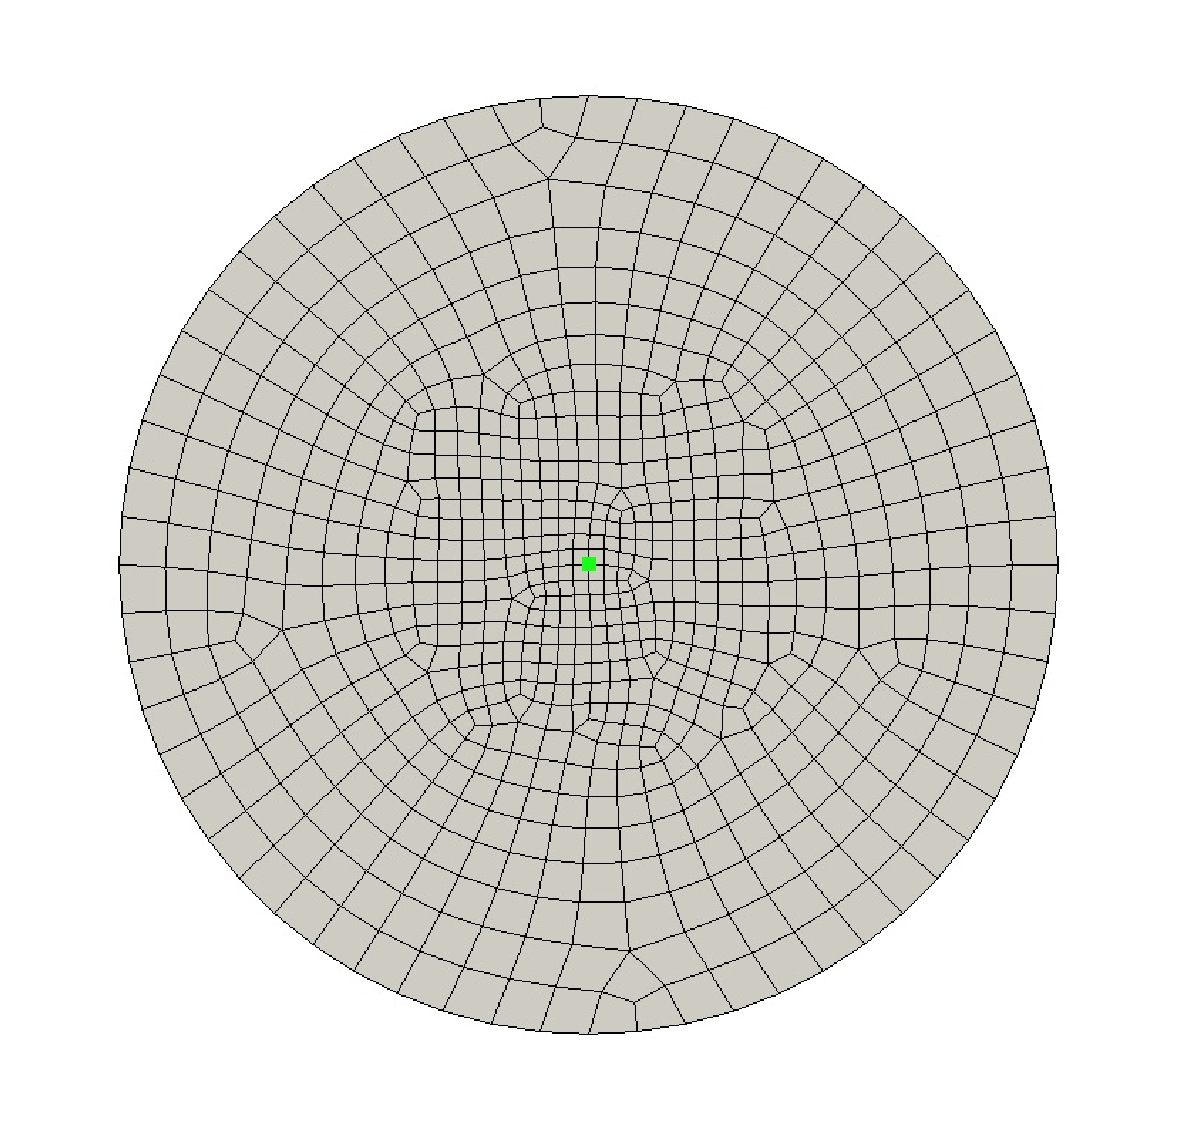
\includegraphics[width=8cm]{bh07.mesh.eps}
\caption{The mesh used in the comparison with Eqn~(\ref{eqn.log.bh}),
  with the green dot indicating the position of the borehole.
  The central elements are $10\times 10$\,m$^{2}$, and the outer
  boundary is at $r=300$\,m.}
\label{bh07.mesh.fig}
\end{figure}



\begin{figure}[htb]
\centering
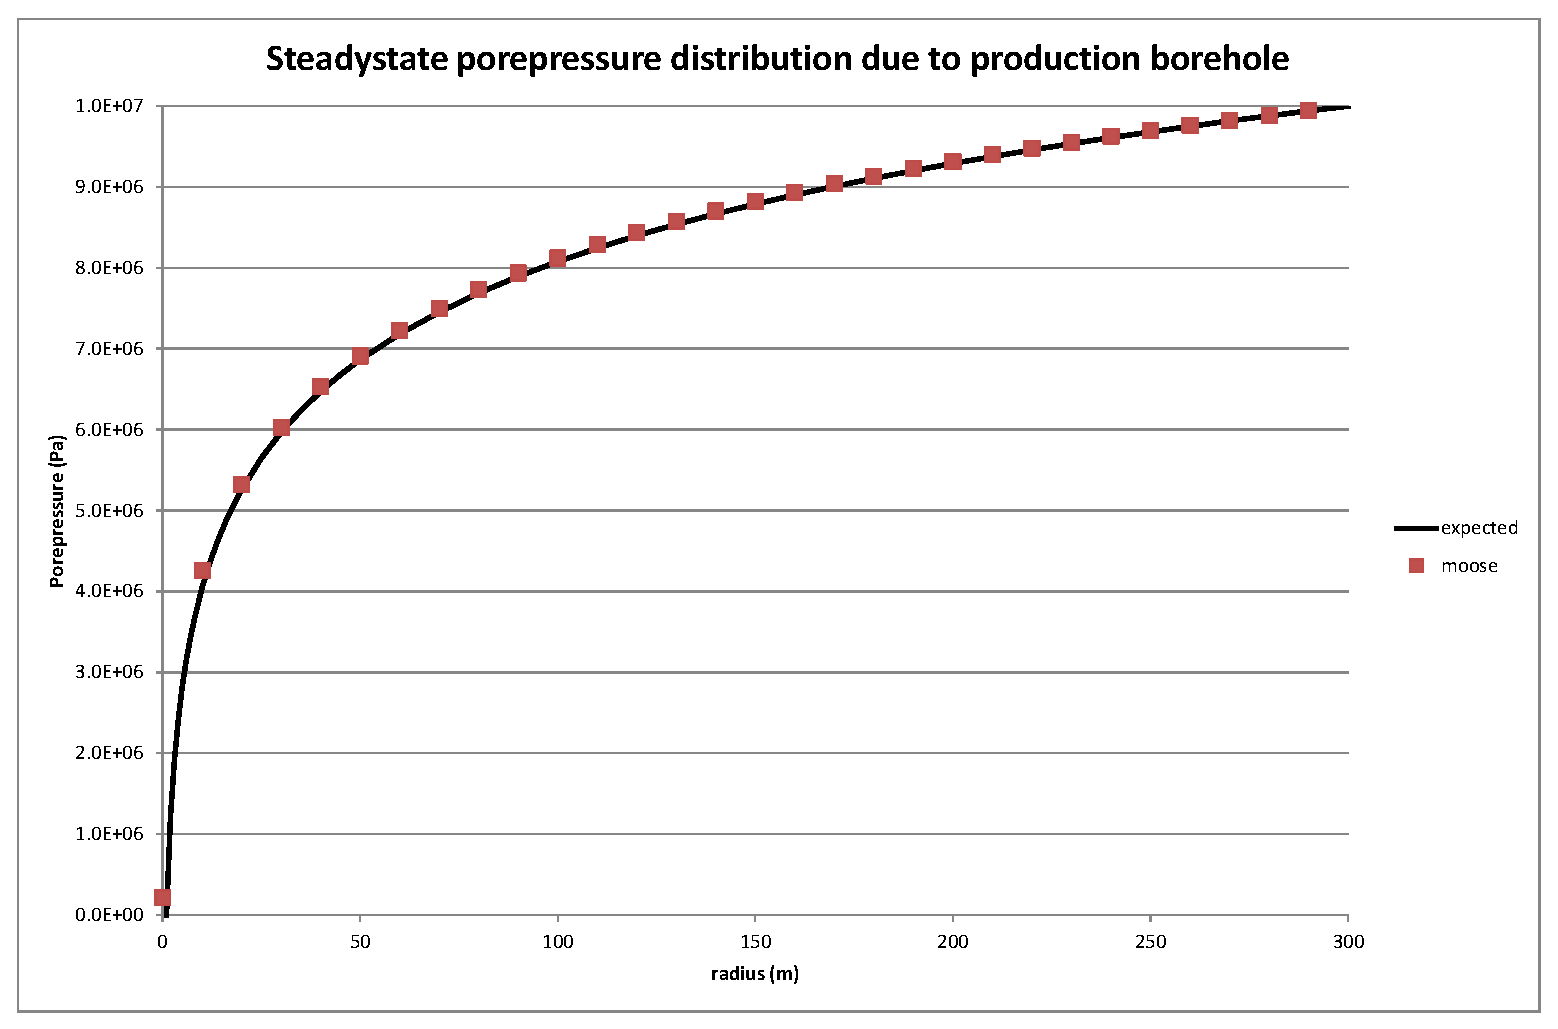
\includegraphics[width=12cm]{bh07.eps}
\caption{Comparison of the MOOSE results (dots) with the analytical
  solution Eqn~(\ref{eqn.log.bh}) for the steadystate porepressure
  distribution surrounding single borehole.}
\label{bh07.fig}
\end{figure}





\chapter{The analytic infiltration solution}
\label{bw}

The Richards' equation for an incompressible fluid reads in one
spatial dimension ($z$) reads 
\begin{equation}
\dot{S} = \nabla \left(D \nabla S\right) - \nabla K \ ,
\end{equation}
where
\begin{eqnarray}
D(S) & = & -\frac{\kappa \kappa_{rel}}{\mu\phi}P_{\mathrm{c}}' \ ,
\\
K(S) & = &\frac{\rho g \kappa\kappa_{\mathrm{rel}}}{\mu\phi} \ .
\end{eqnarray}
Here $P_{\mathrm{c}} = -P$ which is the capillary pressure, and recall
that $P_{\mathrm{c}}'(S)<0$.

The analytic solution of this nonlinear diffusion-advection relevant
to constant infiltration to groundwater has been derived Broadbridge
and White\footnote{P Broadbridge, I White ``Constant rate rainfall
  infiltration: A versatile nonlinear model, 1 Analytical solution''.
  Water Resources Research 24 (1988) 145--154.} for certain functions
$D$ and $K$.  The setup is shown in ``Experiment 1'' of
Figure~\ref{rd_setup.fig} (ignore the specified infiltration rate,
initial saturation and height of sample).  Broadbridge and White
assume the hydraulic conductivity is
\begin{equation}
K(S) = K_{n} + (K_{s}-K_{n})\frac{\Theta^{2}(C-1)}{C-\Theta} \ ,
\end{equation}
where 
\begin{equation}
\Theta = \frac{S - S_{n}}{S_{s} - S_{s}} \ ,
\end{equation}
and the parameters obey $0 \leq K_{n} < K_{s}$, $0 \leq S_{n} \leq S
\leq S_{s}\leq 1$, and $C>1$.  The diffusivity is of the form
$a(b-S)^{-2}$.  This leads to very complicated relationships between
the capillary pressure, $P_{c}$, and the saturation, except in the
case where $K_{n}$ is small, when they are related through
\begin{equation}
\frac{P_{\mathrm{c}}}{\lambda_{s}} = \frac{1-\Theta}{\Theta} - \frac{1}{C}\log
\left( \frac{C-\Theta}{(C-1)\Theta} \right) \ ,
\end{equation}
with $\lambda_{s}>0$ being the final parameter.

Broadbridge and White derive time-dependent solutions for constant
recharge to one end of a semi-infinite line.  This represents constant
rainfall recharge to an initially unsaturated soil block, for
instance.  Their solutions are quite lengthy, so I will not write them
here.  To compare with MOOSE, I use the following parameters --- the
hydraulic parameters are those used in Figure~3 of Broadbridge and
White:
\begin{center}
\begin{tabular}{|ll|}
\hline
Bar length & 20\,m \\
Bar porosity & 0.25 \\
Bar permeability & 1 \\
\hline
Gravity & 0.1\,m.s$^{-2}$ \\
\hline
Fluid density & 10\,kg.m$^{-3}$ \\
Fluid viscosity & 4\,Pa.s \\
\hline
$S_{n}$ & 0\,m.s$^{-1}$ \\
$S_{s}$ & 1\,m.s$^{-1}$ \\
$K_{n}$ & 0\,m.s$^{-1}$ \\
$K_{s}$ & 1\,m.s$^{-1}$ \\
$C$ & 1.5 \\
$\lambda_{s}$ & 2\,Pa \\
\hline
Recharge rate $R_{\ast}$ & 0.5 \\
\hline
\end{tabular} \\
\end{center}
Broadbridge and white consider the case where the initial condition is
$S=S_{s}$, but this yields $P=-\infty$, which is impossible to use in
a MOOSE model.  Therefore the initial condition $P=-900$\,Pa is used
which avoids any underflow problems.  The recharge rate of
$R_{\ast}=0.5$ corresponds in the MOOSE model to a recharge rate of
$0.5\rho\phi(\kappa_{s}-\kappa_{n})=1.25$\,kg.m$^{-2}$.s$^{-1}$.  Note
that I've chosen $\frac{\rho g \kappa}{\mu \phi} = 1$\,m.s$^{-1}$, so
that the $K_{n}$ and $K_{s}$ may be encoded as $\kappa_{n}=0$ and
$\kappa_{s}=1$ in the relative permeability function
Eqn~(\ref{bw.krel}) in a straightforward way.

Figure~\ref{bw.fig} shows good agreement between the analytic solution
of Broadbridge and White and the MOOSE implementation.  There are
minor discrepancies for small values of saturation: these get smaller
as the temporal and spatial resolution is increased, but never totally
disappear due to the initial condition of $P=-900$\,Pa.

Two tests (with and without mass lumping) are part of the automatic
test suite that is run every time the code is updated.

\begin{figure}[htb]
\centering
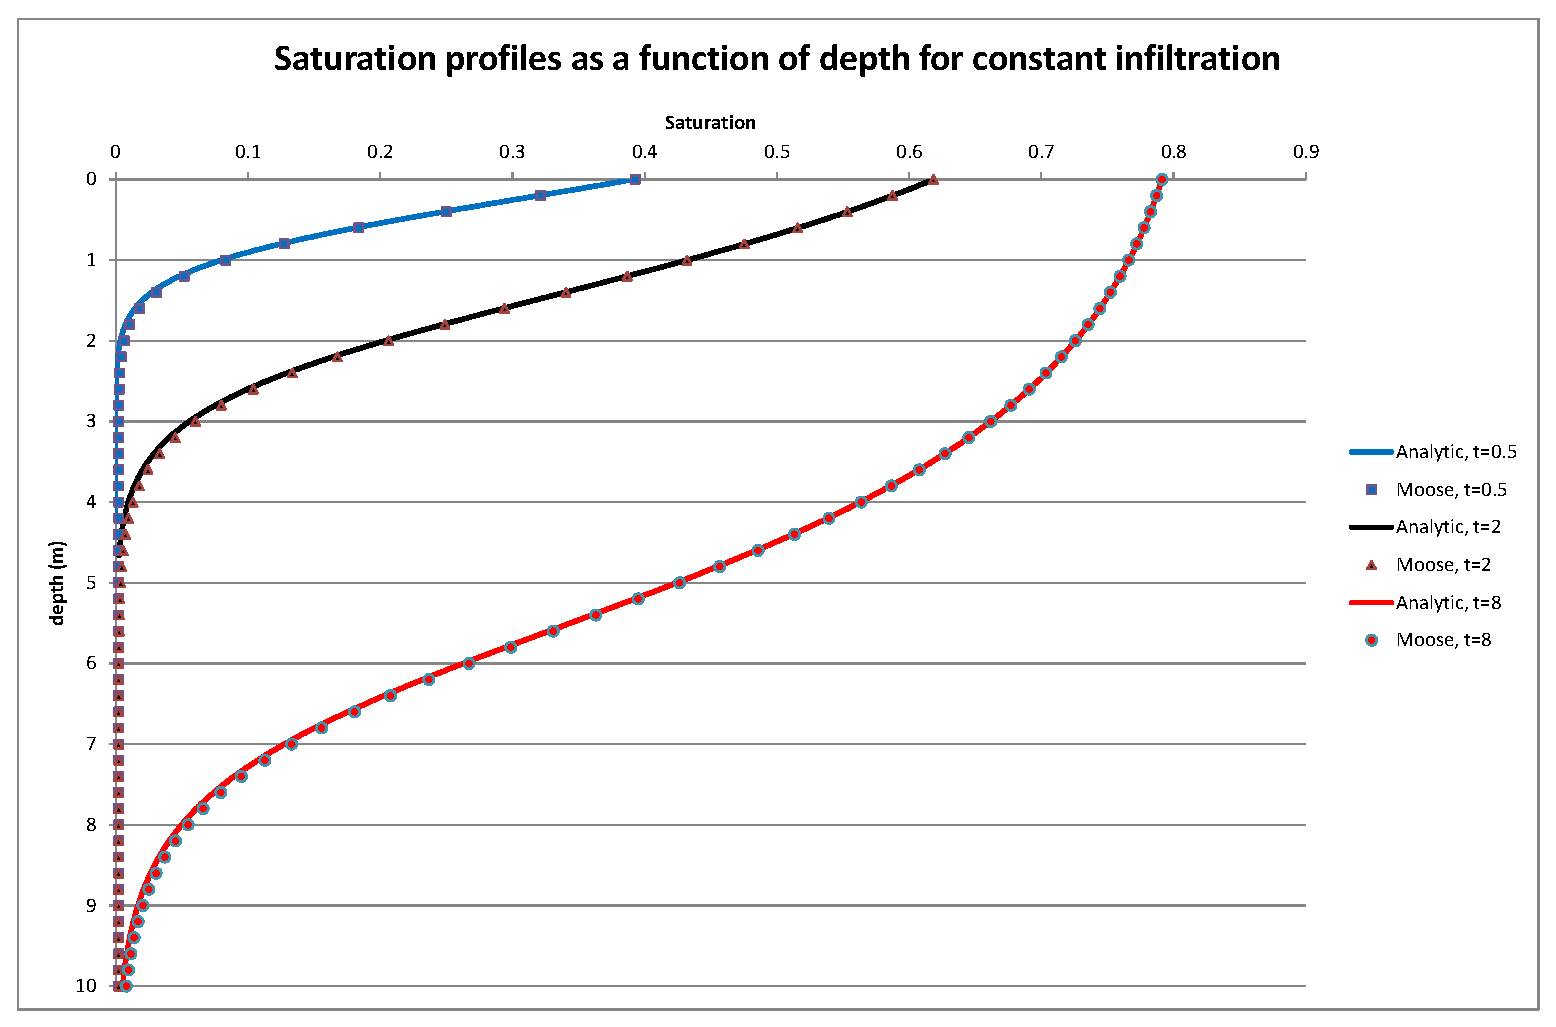
\includegraphics[width=16cm]{bw.eps}
\caption{Comparison of the Broadbridge and White analytical solution
  with the MOOSE solution for 3 times.  This figure is shown in the
  standard format used in the Broadbridge-White paper: the constant
  recharge is applied to the $\mbox{depth}=0$ surface, and gravity
  acts downwards in this figure.}
\label{bw.fig}
\end{figure}





\chapter{The analytic drainage solution}
\label{wli}

Warrick, Lomen and Islas\footnote{AW Warrick, DO Lomen and A Islas,
  ``An analytical solution to Richards' Equation for a Draining Soil
  Profile'', Water Resources Research 26 (1990) 253--258.} extended
the analysis of Broadbridge and White (Chapter~\ref{bw}) to include
the case of drainage from a medium.  The setup is in ``Experiment 2'' of
Figure~\ref{rd_setup.fig}.  To obtain their analytical
solutions, Warrick, Lomen and Islas make the same assumptions as
Broadbridge and White concerning the diffusivity and conductivity of
the medium.  Their solutions are quite lengthy, so I will not write
them here.

A MOOSE model with the parameters almost identical to those listed in
Chapter~\ref{bw} is compared with the analytical solutions.  The only
differences are that the ``bar'' length is 10000\,m (to avoid any
interference from the lower Dirichlet boundary condition), and
$R_{\ast}=0$ since there is no recharge.  The initial condition is
$P=10^{-4}$\,Pa: the choice $P=0$ leads to poor convergence since
by construction the Broadbridge-White capillary function is only
designed to simulate the unsaturated zone $P<0$ and a sensible
extension to $P\geq 0$ is discontinuous at $P=0$.

Figure~\ref{wli.fig} shows good agreement between the analytic
solution and the MOOSE implementation.  Any minor discrepancies get
smaller as the temporal and spatial resolution increase.

This test is part of the automatic test suite that is run every time
the code is updated.


\begin{figure}[htb]
\centering
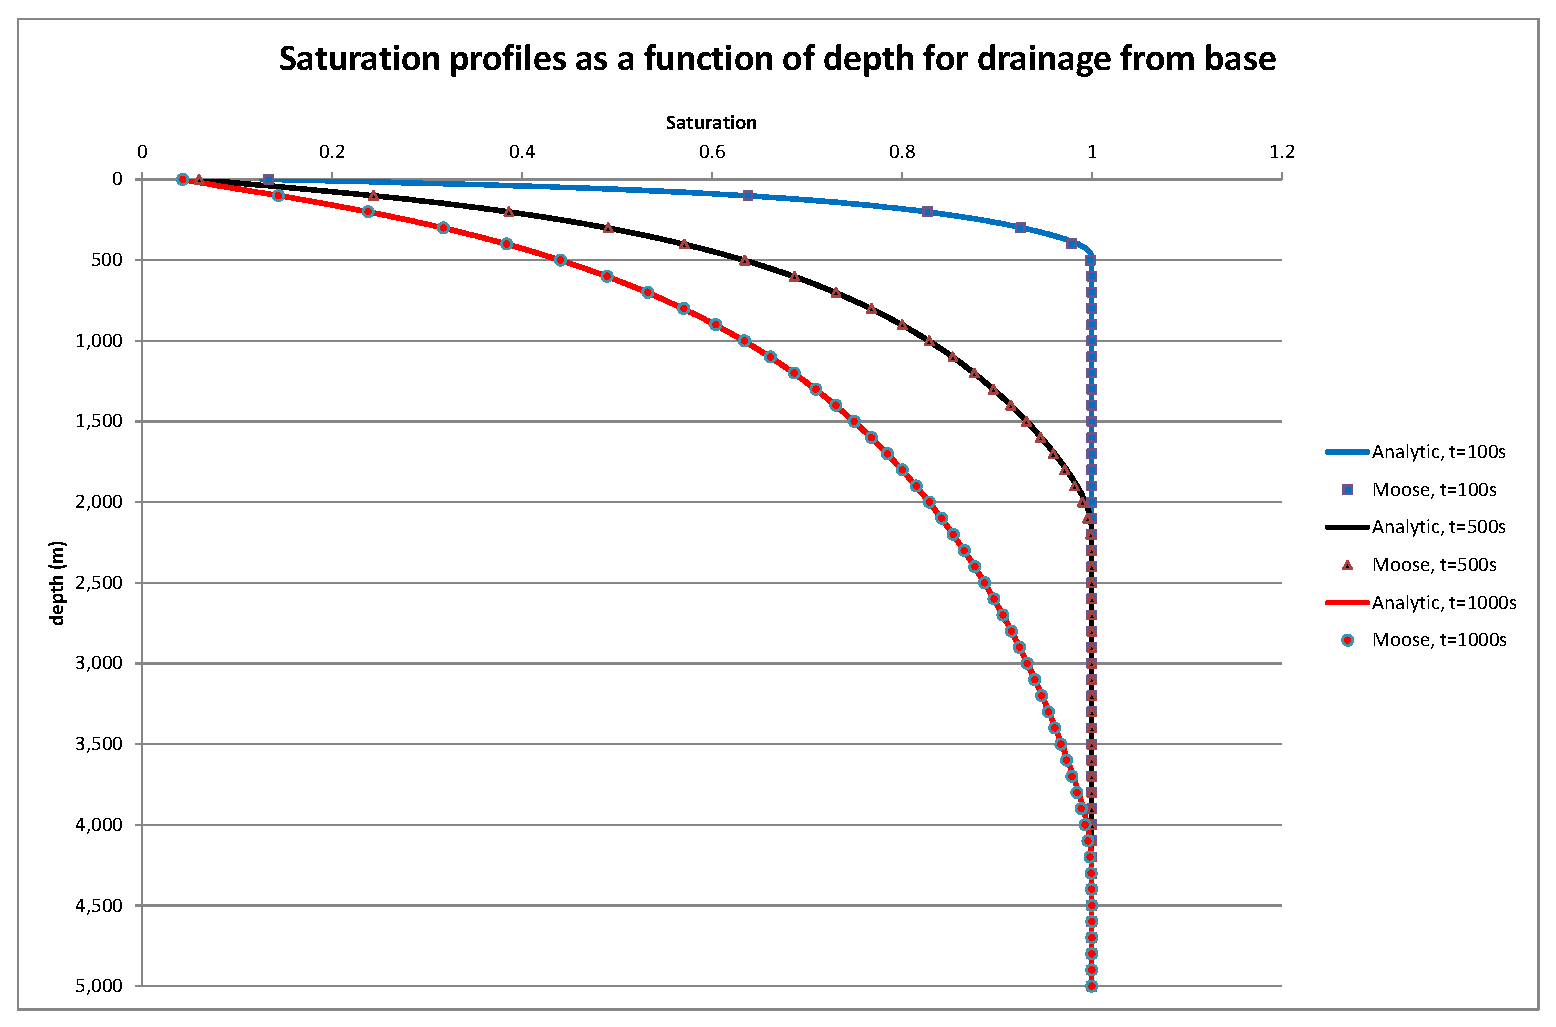
\includegraphics[width=16cm]{wli.eps}
\caption{Comparison of the Warrick, Lomen and Islas analytical solution
  with the MOOSE solution for 3 times.  This figure is shown in the
  standard format used in the literature: the top of the model is
  $\mbox{depth}=0$ surface, and gravity acts downwards in this figure,
with fluid draining from $\mbox{depth}=\infty$.}
\label{wli.fig}
\end{figure}




\chapter{Infiltration and drainage}
\label{forsyth}

Forsyth, Wu and Pruess\footnote{PA Forsyth, YS Wu and K Pruess,
  ``Robust numerical methods for saturated-unsaturated flow with dry
  initial conditions in heterogeneous media'', Advances in Water
  Resources 18 (1995) 25--38} describe a HYDRUS simulation of an
experiment involving infiltration (experiment 1) and subsequent
drainage (experiment 2) in a large caisson.  The simulation is
effectively one dimensional, and is shown in
Figure~\ref{rd_setup.fig}.

\begin{figure}[htb]
\begin{center}
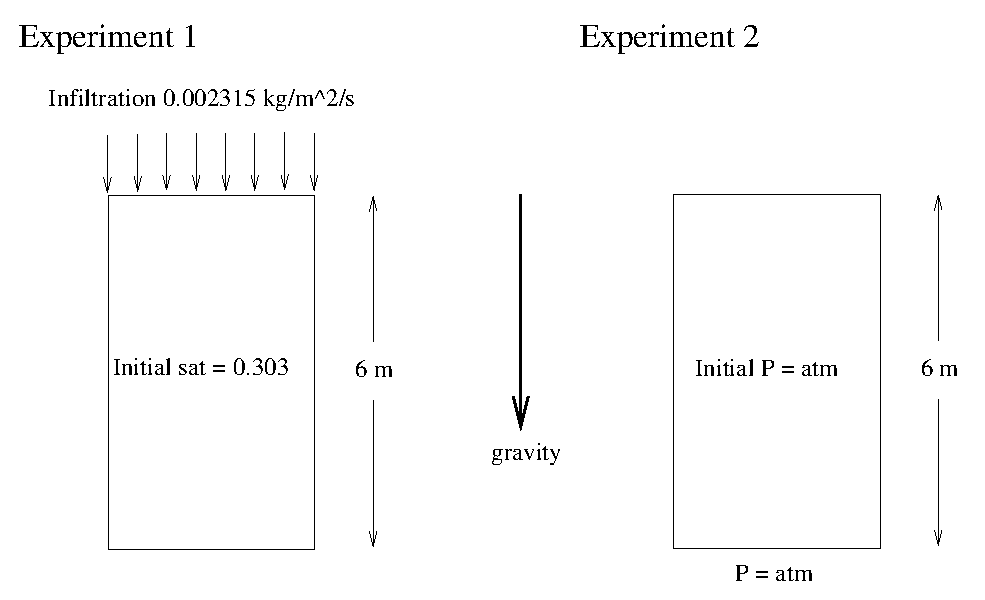
\includegraphics[width=12cm]{rd_setup.eps}
\caption{Two experimental setups from Forsyth, Wu and Pruess.
  Experiment 1 involves infiltration of water into an initially
  unsaturated caisson.  Experiment 2 involves drainage of water from
  an initially saturated caisson.}
\label{rd_setup.fig}
\end{center}
\end{figure}

The properties common to each experiment
are:
\begin{center}
\begin{tabular}{|ll|}
\hline
Caisson & 0.33 \\
Caisson permeability & $2.95\times 10^{-13}$\,m$^{2}$ \\
\hline
Gravity & 10\,m.s$^{-2}$ \\
\hline
Water density & 1000\,kg.m$^{-3}$ \\
Water viscosity & 0.00101\,Pa.s \\
Water bulk modulus & 20\,MPa \\
Water immobile saturation & 0.0 \\
Water residual saturation & 0.0 \\
Air residual saturation & 0.0 \\
Air pressure & 0.0 \\
\hline
van Genuchten $\alpha$ & $1.43\times 10^{-4}$\,Pa$^{-1}$ \\
van Genuchten $a$ & 0.336 \\
van Genuchten\_1 cutoff & 0.99 \\
\hline
\end{tabular} \\
\end{center}
In each experiment 120 finite elements were used along the length of
the Caisson.  The modified van-Genuchten relative permeability curve
was employed in order to improve convergence significantly.  Hydrus
also uses a modified van-Genuchten curve, although I couldn't find any
details on the modification.

In experiment 1, the caisson is initially at saturation 0.303
($P=-72620.4$\,Pa), and water is pumped into the top with a rate
0.002315\,kg.m$^{-2}$.s$^{-1}$.  This causes a front of water to
advance down the caisson.  Figure~\ref{rd.result.fig} shows the
agreement between MOOSE and the published result (this result was
obtained by extracting data by hand from online graphics).

In experiment 2, the caisson is initially fully saturated at $P=0$,
and the bottom is held at $P=0$ to cause water to drain via the action
of gravity.  Figure~\ref{rd.result.fig} shows the agreement between
MOOSE and the published result.

Experiment 1 and the first 4 simulation days of experiment 2 are
marked as ``heavy'' in the Richards' test suite since the simulations
take around 3 seconds to complete.  This means they are not run by
default every time the code is updated, and must be run manually.
However, the final 96 days of experiment 2 run quickly and are part of
the automatic test suite.


\begin{figure}[htb]
\begin{center}
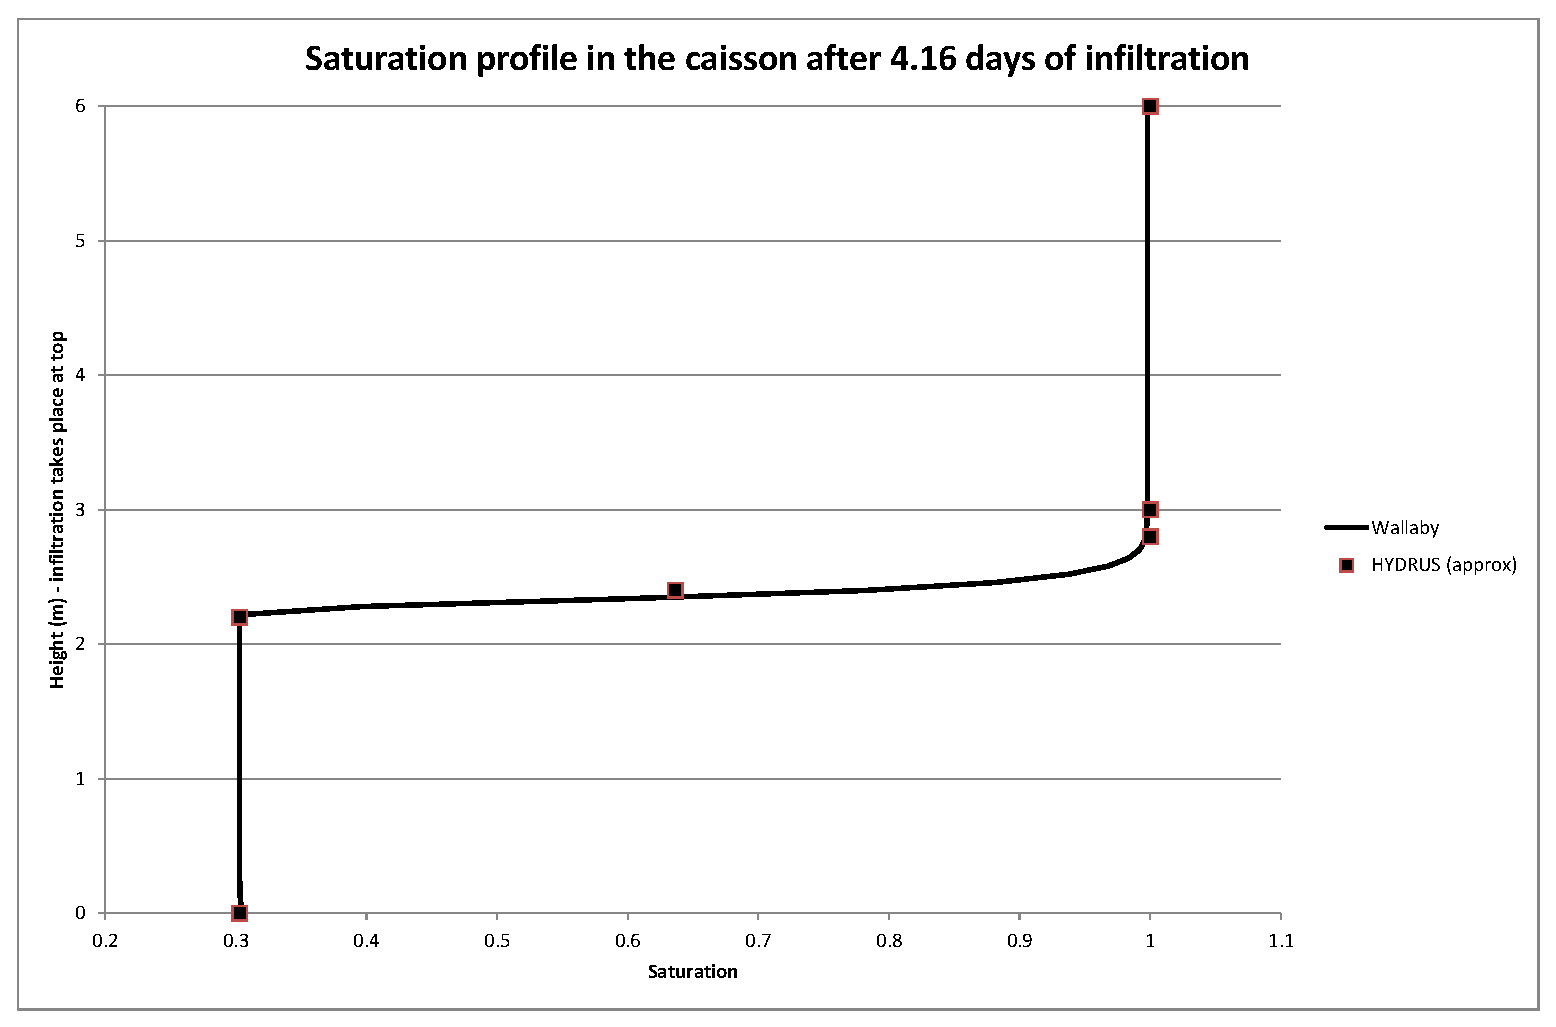
\includegraphics[width=12cm]{rd01.eps} \\
$\mbox{}$\\
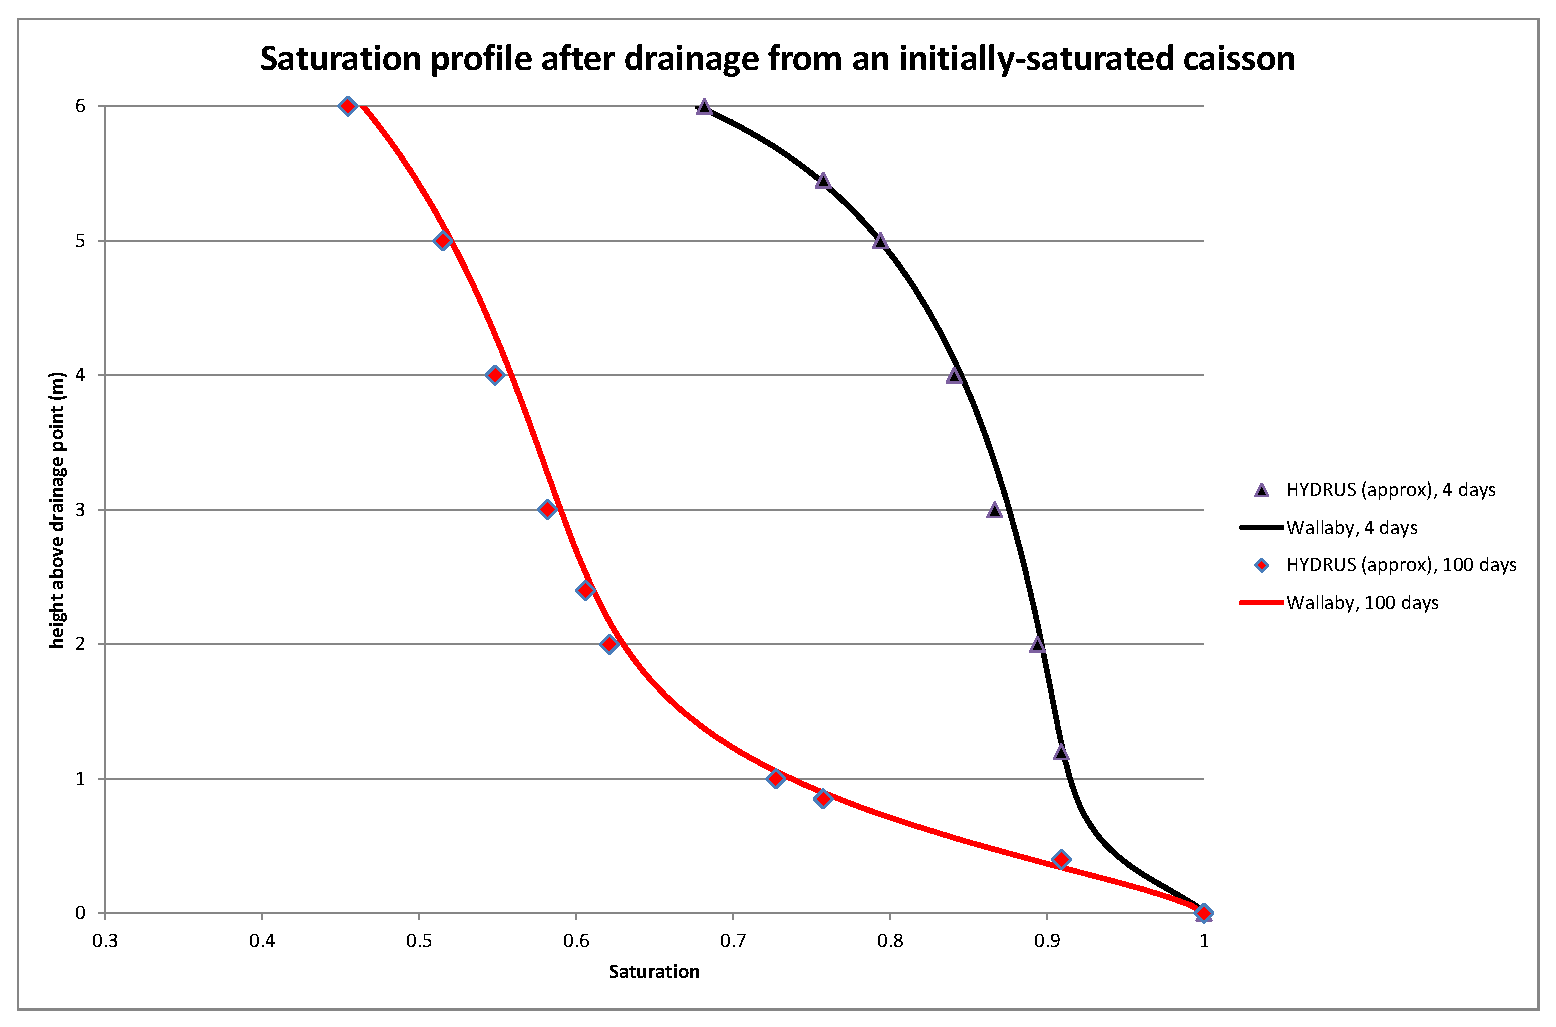
\includegraphics[width=12cm]{rd02.eps}
\caption{Saturation profiles in the caisson.  Top: After 4.16 days of
  infiltration.  Bottom: After drainage from an initially-saturated
  simulation (4 days and 100 days profiles).  Note that the HYDRUS
  results are only approximate as I extrated the data by hand from
  online graphics.}
\label{rd.result.fig}
\end{center}
\end{figure}


\chapter{The single-phase Buckley-Leverett problem}
\label{bl}

MOOSE is compared with a simple single-phase one-dimensional
Buckley-Leverett problem\footnote{SE Buckley and MC Leverett (1942)
  ``Mechanism of fluid displacements in sands''.  Transactions of the
  AIME {\bf 146} 107--116}.  The single-phase fluid moves in a region
$0\leq x\leq 15$\,m.  A fully-saturated front initially sits at
position $x=5$, while the region $x>5$ is initially unsaturated.  With
zero suction function $P_{c} = 0$, there is no diffusion of the sharp
front, and it progresses towards the right.  This is a difficult
problem to simulate numerically as maintaining the sharp front is
hard.  The front's speed is independent of the relative permeability,
since the fluid is flowing from a fully-saturated region (where
$\kappa_{\mathrm{rel}}=1$).  This problem is therefore a good test of
the upwinding.


In the simulation below, the pressure at the left boundary is kept
fixed at $P_{0}=0.98$\,MPa, while the right boundary is kept fixed at
$P_{15}=-20000$\,Pa, so the difference is 1\,MPa.  The medium's
permeability is set to $\kappa = 10^{-10}\,\mathrm{m}^{2}$ and its
porosity is $\phi = 0.15$.  It is not possible to use a zero suction
function in the MOOSE implementation, but using the van Genuchten
parameters $\alpha = 10^{-3}$\,Pa$^{-1}$ and $m=0.8$ approximates it.
The fluid viscosity is $\mu = 10^{-3}$\,Pa.s.

The initial condition is
\begin{equation}
P(t=0) = \left\{
\begin{array}{ll}
P_{0} - (P_{0}-P_{15})x/5 & \ \ \ \mbox{for }\ \ x<5 \\
P_{15} & \ \ \ \mbox{for }\ \ x\geq 5  
\end{array}
\right. \ ,
\end{equation}
which is shown in
Figure~\ref{bl_setup.figa}.  With the suction function defined above
this gives
\begin{equation}
S(t=0) = \left\{
\begin{array}{ll}
1 & \ \ \ \mbox{for }\ \ x\leq 4.9 \\
0.061 & \ \ \ \mbox{for} \ \ x \geq 5
\end{array}
\right.
\end{equation}

\begin{figure}[htb]
\begin{center}
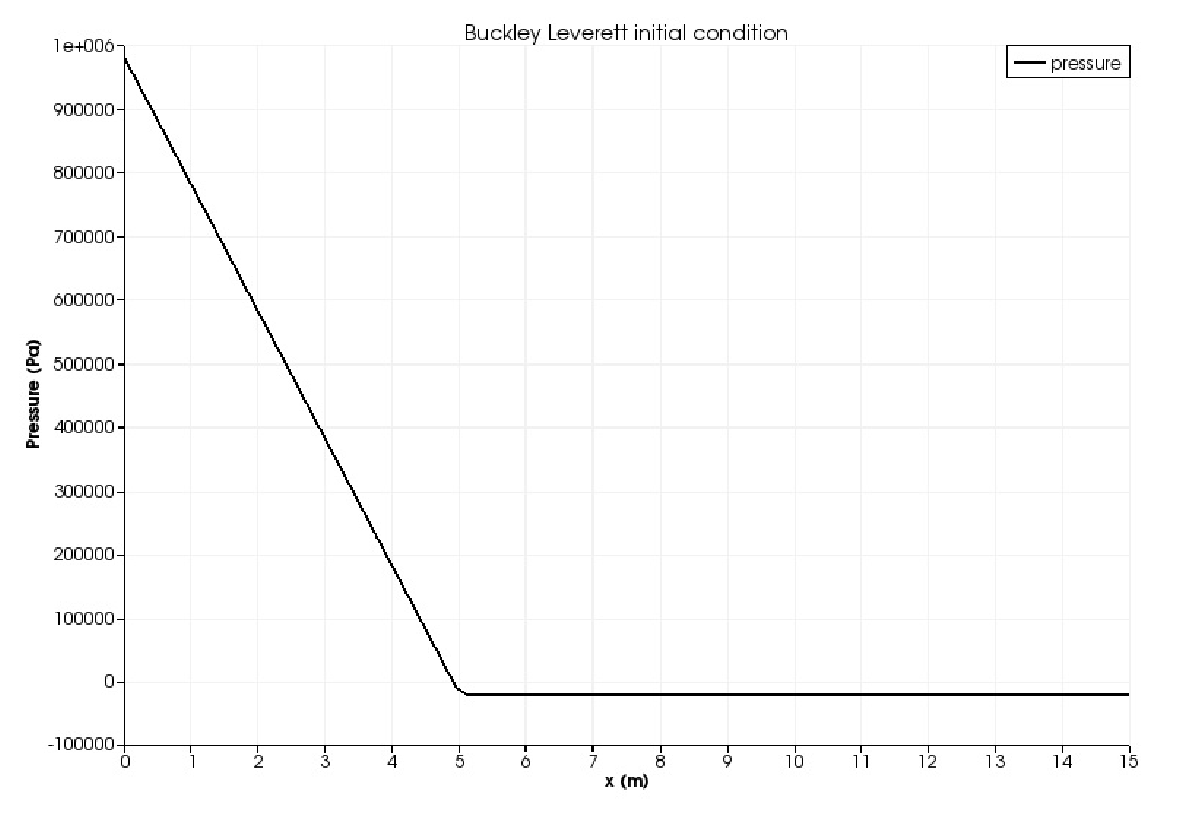
\includegraphics[width=12cm]{bl_initial.eps}
\caption{Initial setup of the Buckley-Leverett problem where
  porepressure is a piecewise linear function.  The region
$x\leq 4.9$ is fully saturated, while the region $x>5$ has saturation
  0.061.  During simulation the value $P(x=0)=0.98\times 10^{6}$\,MPa
  is held fixed.}
\label{bl_setup.figa}
\end{center}
\end{figure}

Good approximations for the pressure $P(x,t)$
and the front position $f(t)$ may be determined from
\begin{eqnarray}
\frac{{\mathrm d} f}{{\mathrm d} t} & = & -\frac{\kappa}{\phi\mu}
\left.\frac{\partial  P}{\partial x}\right|_{x = f} \ , \nonumber \\
P(x,t) & = & \left\{
\begin{array}{ll}
P_{0} - (P_{0}-P_{15})x/f & \mbox{ for } x\leq f  \\
P_{15} & \mbox{ for } x>f 
\end{array}
\right. \ ,
\label{eqn.predicted.bl.posn.eqna}
\end{eqnarray}
which has solution
\begin{equation}
f(t) = \sqrt{f(0)^{2} + \frac{2\kappa}{\phi\mu}(P_{0}-P_{15})t} \ .
\end{equation}
For the parameters listed above, the front will be at position
$f=9.6$\,m at $t=50$\,s.  This solution is only valid for zero
capillary suction.  A nonzero suction function will tend to diffuse
the sharp front.

With coarse meshes it is impossible to simulate a sharp front, of
course, since the front is spread over at least one element.  It can be
therefore quite advantageous to use mesh adaptivity in this test,
since the mesh can be fine around the front where all the interesting
dynamics occurs, and coarse elsewhere.

Figure~\ref{satfront.figa} shows the results from a MOOSE simulation
with a uniform mesh of size 0.1\,m.  At $t=50$\,s the front in this
simulation sits at $x=9.6$\,m as desired.  However, the simulation
takes 3 minutes to complete due to the very low values of saturation
obtained for van Genuchten $\alpha=10^{-3}$\,Pa$^{-1}$.  Other
simulations give similar results but run much faster.  For instance,
great speedups can be obtained by setting the van-Genuchten parameter
$\alpha=10^{-4}$\,Pa$^{-1}$, but the front diffuses a little into the
unsaturated region.  Using an initial mesh of element size 1\,m, and a
minimum size of 0.125\,m, with a maximum timestep of 0.3\,s (to give
the mesh time to adapt around the front),the front at $t=50$\,s sits
between between $x=9.9$\,m and $x=10.35$\,m, and the simulation takes
only 3 seconds.  The automatic test suite contains two simulations
(with and without mass lumping) with
elements of size 0.1\,m using a timestep of 2\,s, which gives results
very similar to these, and takes less than 2 seconds to run.

\begin{figure}[htb]
\begin{center}
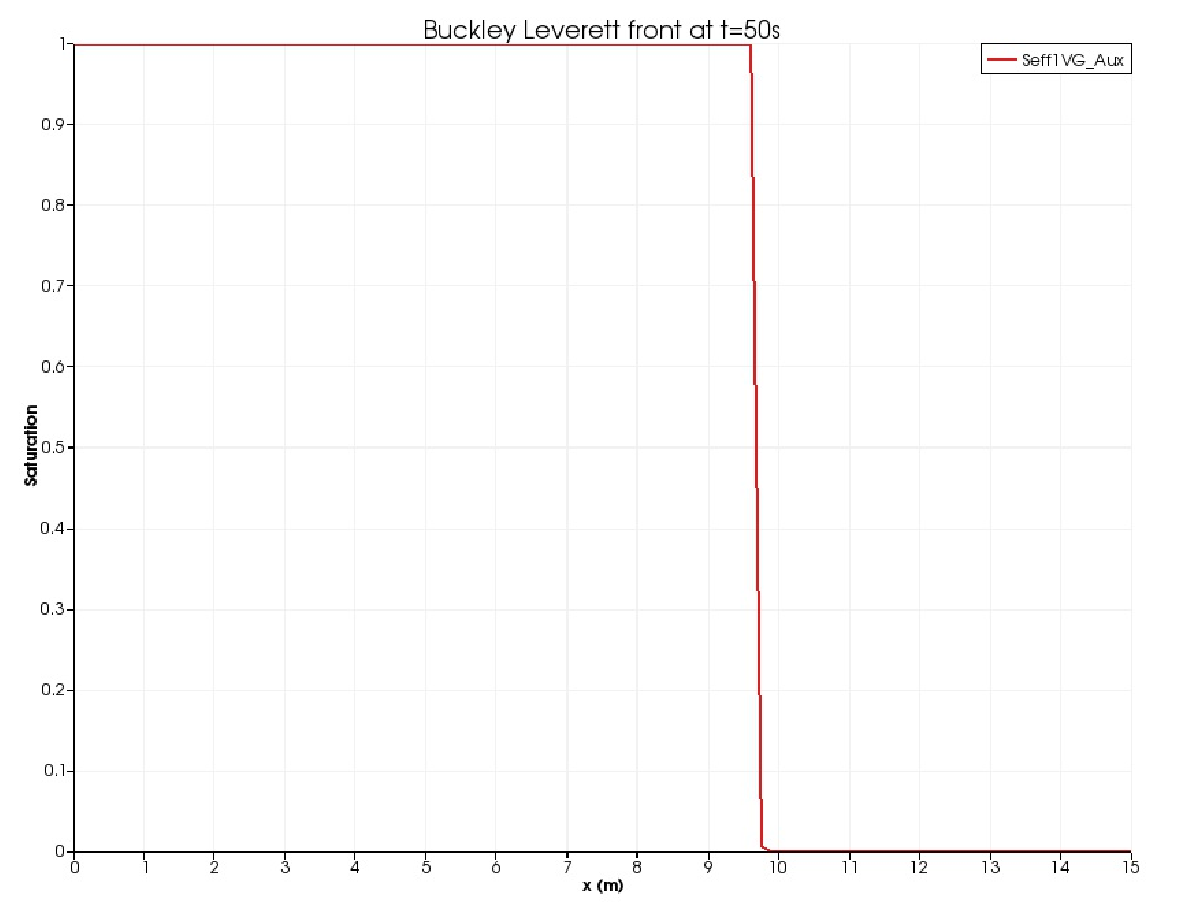
\includegraphics[width=10cm]{bl_seff.eps} \\
$\mbox{}$
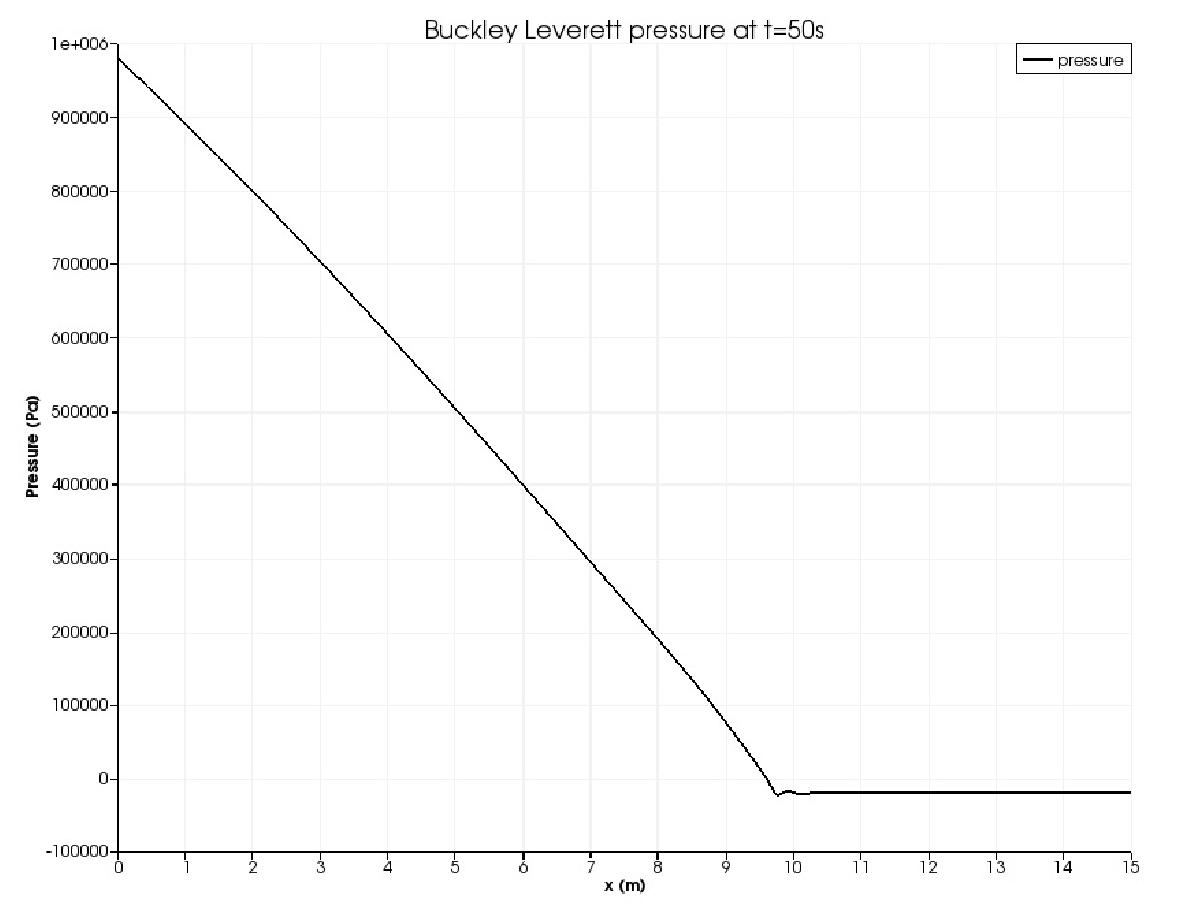
\includegraphics[width=10cm]{bl_p.eps} \\
\caption{The MOOSE solution of the Buckley-Leverett problem at
  $t=50$\,s.  Top: saturation.  Bottom: porepressure.  The front sits
  between $x=9.6$\,m as expected from the analytical solution.}
\label{satfront.figa}
\end{center}
\end{figure}



\chapter{An excavation}
\label{ex}

``Excavations'' are important in underground mining simulations.
These are voids underground created by mining of material.  On the
boundary of the void the porepressure is fixed to a user-defined
value, typically atmostpheric pressure.  The size of the void changes
with time as material is progressively mined.  As discussed in the
Theory Manual, these time-dependent boundary conditions are
conveniently defined through a function.  This section demonstrates
that this procedure works as expected.

As depicted in Figure~\ref{ex02_3D_mesh.fig}, a 3D simulation is run
with region in the middle of the mesh that will be excavated.  The
simulation is run for $3\times 10^{7}$\,s which is the time taken to
excavate the entire panel.  Figure~\ref{ex02.fig} shows the
porepressure distribution at the plane of the panel at two times, and
demonstrates that the correct boundary conditions are being applied.

\begin{figure}[htb]
\centering
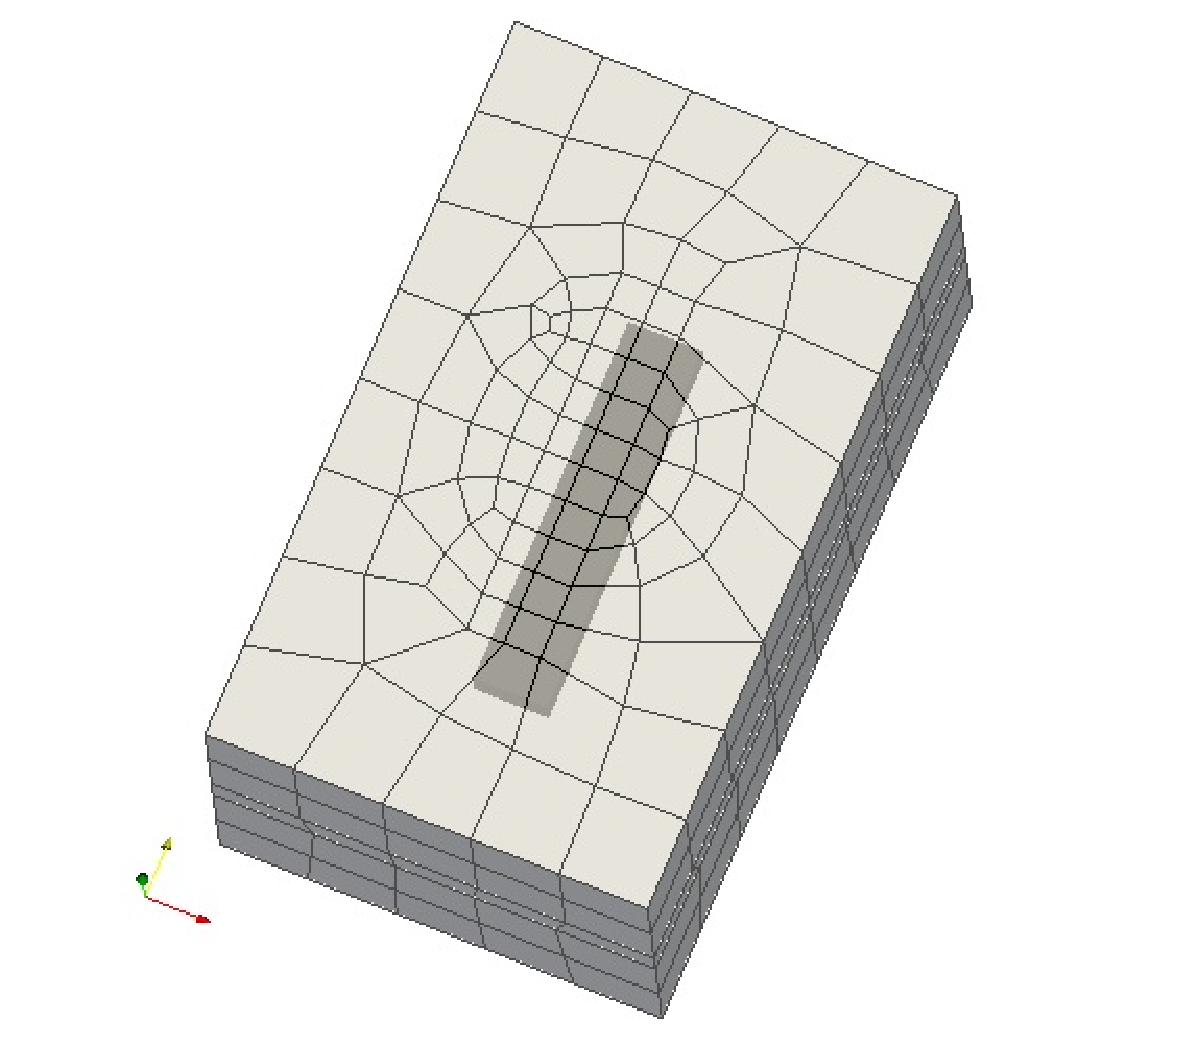
\includegraphics[width=10cm]{ex02_3D_mesh.eps}
\caption{The 3D mesh used in the excavation test.  This view is
  looking down on the mesh.  In the middle of
  the solid there is a region that is excavated, and this is shown in
  a darker colour.}
\label{ex02_3D_mesh.fig}
\end{figure}

\begin{figure}[htb]
\centering
\begin{tabular}{cc}
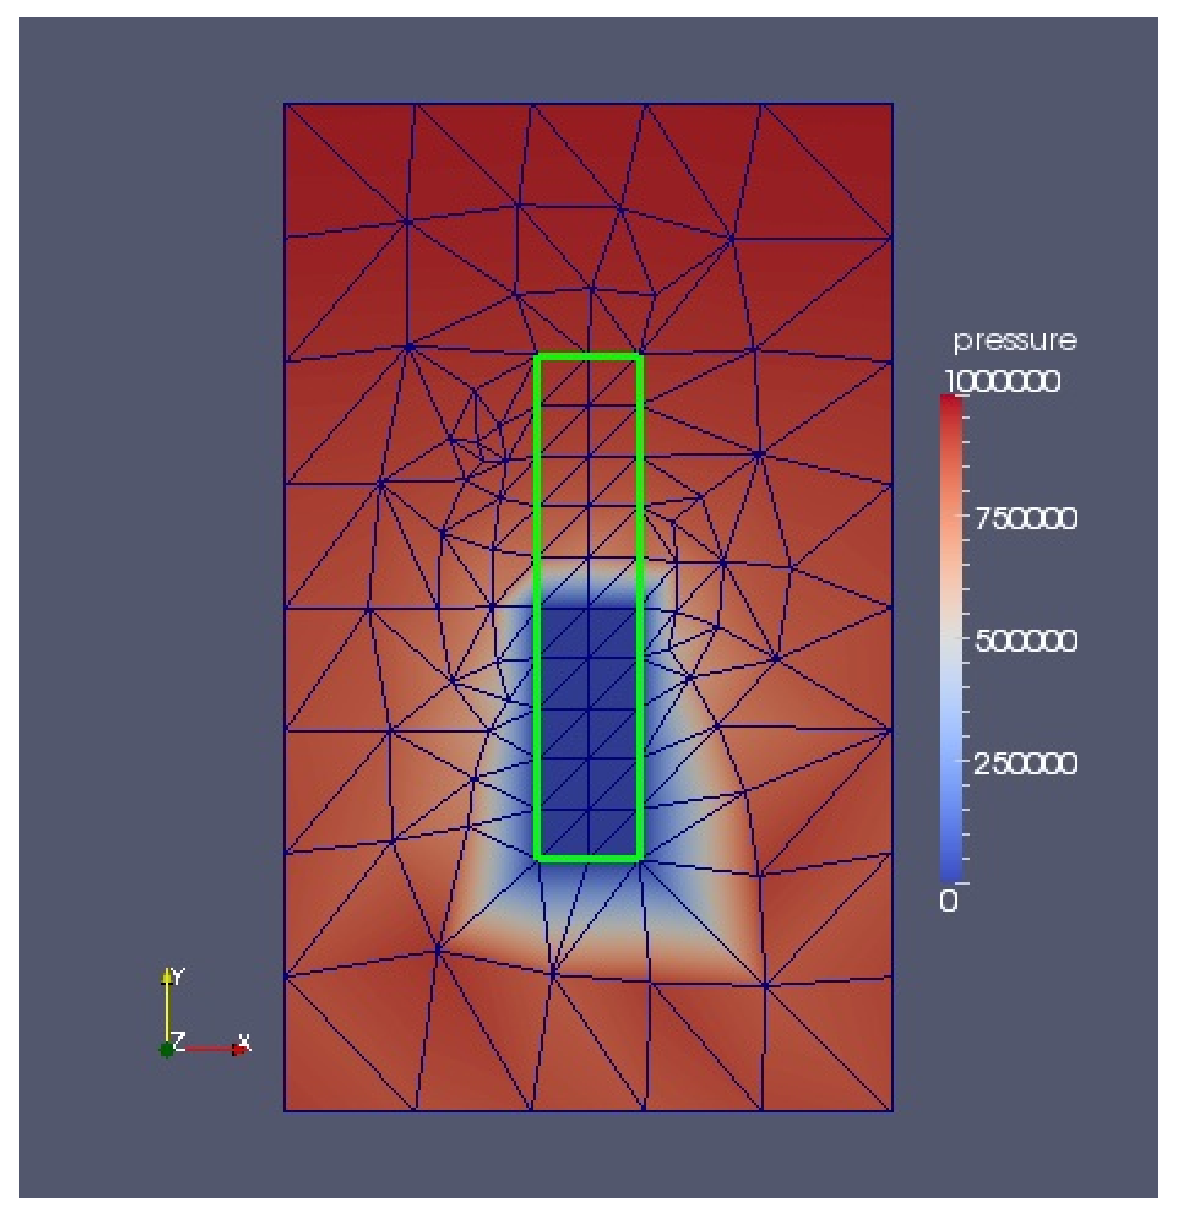
\includegraphics[width=8cm]{ex02_1.5.eps} &
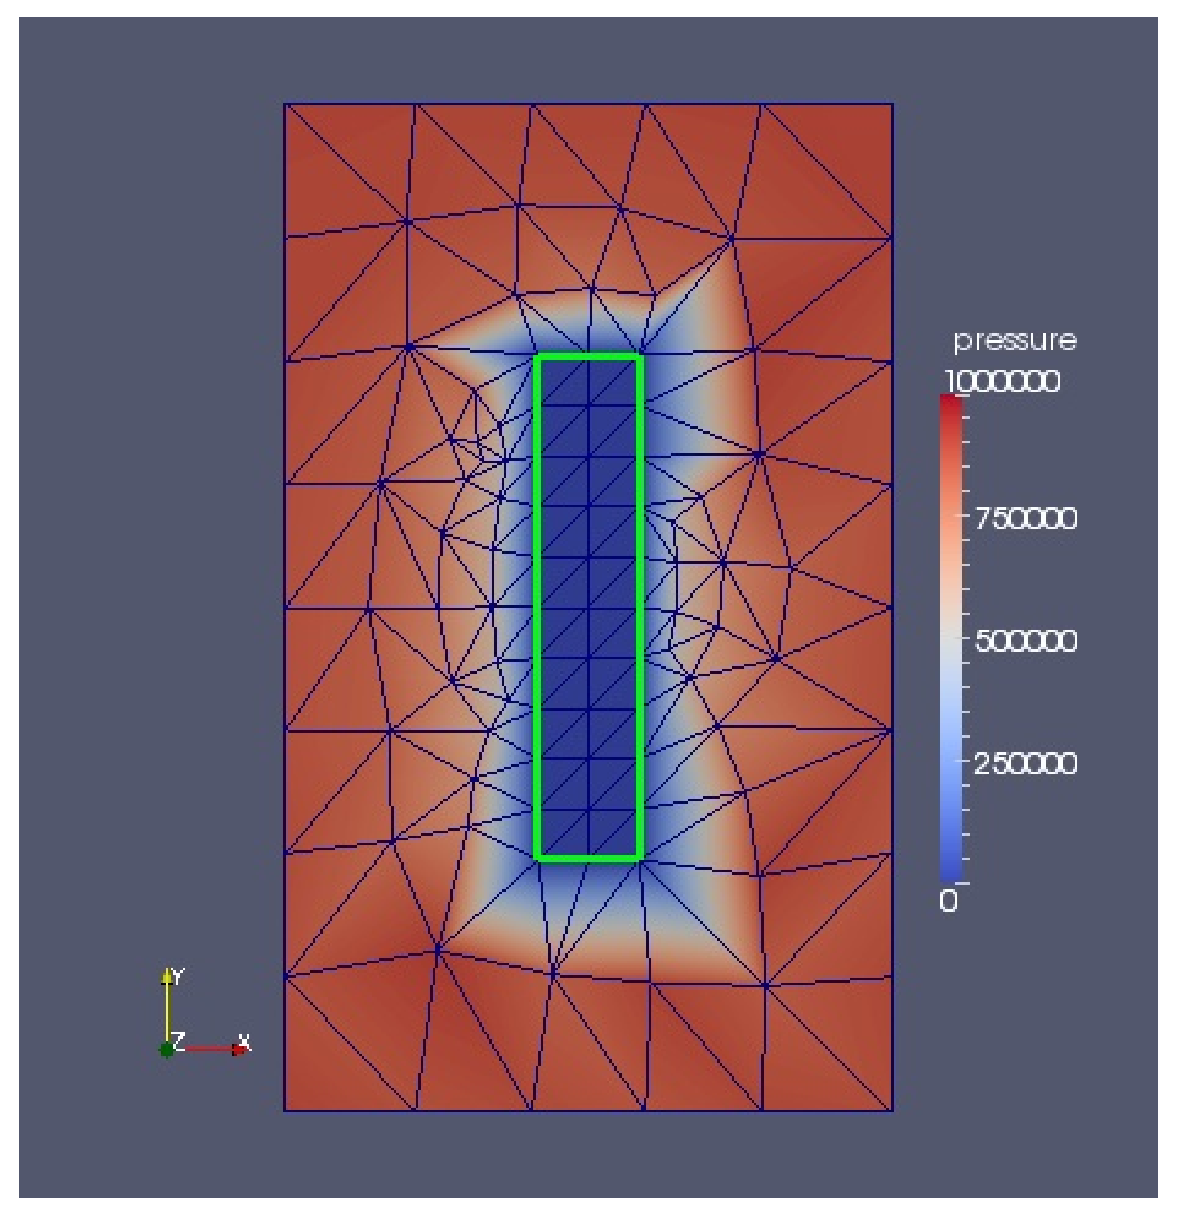
\includegraphics[width=8cm]{ex02_3.eps}
\end{tabular}
\caption{The porepressure contoured on a horizontal slice through the
  excavation region.  The excavation region is shown as a green
  rectangle.  The excavation is completed in $3\times 10^{7}$\,s and
  has $P=0$ on the boundary.  The left figure shows the porepressure
  at $t=1.5\times 10^{7}$\,s, and the right figure shows $t=3\times
  10^{7}$\,s.}
\label{ex02.fig}
\end{figure}




\chapter{Water infiltration into a two-phase system}
\label{rsc}

An analytic solution of the two-phase Richards' equations with gravity
on a semi-infinite line $z\geq 0$, with a constant water infiltration
flux at $z=0$ has been derived by Rogers, Stallybrass and
Clements~\footnote{C Rogers, MP Stallybrass and DL Clements ``On two
  phase filtration under gravity and with boundary infiltration:
  application of a Backlund transformation'' Nonlinear Analysis,
  Theory, Methods and Applications 7 (1983) 785--799}.  The setup is
very similar to the left-hand drawing in Figure~\ref{rd_setup.fig},
but ignore the initial saturation and infiltration rate, and the
height of the sample is infinite.  The authors
assume incompressible fluids; linear relative permeability
relationships; the ``oil'' (or ``gas'') viscosity is larger than the
water viscosity; and, a certain functional form for the capillary
pressure.  When the oil viscosity is exactly twice the water
viscosity, their effective saturation reads
\begin{equation}
S_{\mathrm{eff}} = \frac{1}{\sqrt{1 + \exp((P_{c} - A)/B)}} \ ,
\label{eqn.rsc.seff}
\end{equation}
where $P_{c} = P_{\mathrm{oil}}-P_{\mathrm{water}}$ is the capillary
pressure, and $A$ and $B$ are arbitrary parameters to be defined by
the user in the MOOSE implementation.  For other oil/water viscosity
ratios $P_{c} = P_{c}(S_{\mathrm{eff}})$ is more complicated, and note
that their formulation allows $P_{c}<0$, but only
the particular form Eqn~(\ref{eqn.rsc.seff}) need be used to validate
the MOOSE implementation.

RSC's solutions are quite lengthy, so I will not write them here.  To
compare with MOOSE, the following parameters are used:
\begin{center}
\begin{tabular}{|ll|}
\hline
Bar length & 10\,m \\
Bar porosity & 0.25 \\
Bar permeability & $10^{-5}$\,m$^{2}$ \\
\hline
Gravity\footnote{Unfortunately there must be a typo in the RSC paper
  as for nonzero gravity their results are clearly incorrect.} & 0\,m.s$^{-2}$ \\
\hline
Water density & 10\,kg.m$^{-3}$ \\
Water viscosity & $10^{-3}$\,Pa.s \\
\hline
Oil density & 20\,kg.m$^{-3}$ \\
Oil viscosity & $2\times 10^{-3}$\,Pa.s \\
\hline
Capillary $A$ & 10\,Pa \\
Capillary $B$ & 1\,Pa \\
\hline
Initial water pressure & 0\,Pa \\
Initial oil pressure & 15\,Pa \\
Initial water saturation & 0.08181 \\
Initial oil saturation & 0.91819 \\
\hline
Water injection rate & 1\,kg\,s$^{-1}$\,m$^{-2}$ \\
\hline
\end{tabular} \\
\end{center}

In the RSC theory water is injected into a semi-infinite domain,
whereas of course the MOOSE implementation has finite extent ($0\leq z
\leq 10$ is chosen).  Because of the near incompressibility of the
fluids (I choose the bulk modulus to be 2\,GPa) this causes the
porepressures to rise enormously, and the problem can suffer from
precision-loss problems.  Therefore, the porepressures are fixed at
$z=10$.  This does not affect the progress of the water saturation
front.  Figure~\ref{rsc.fig} shows good agreement between the analytic
solution and the MOOSE implementation.  Any minor discrepancies get
smaller as the temporal and spatial resolution increase, as is
suggested by the two comparisons in that figure.

The ``low-resolution'' test, which has 200 elements in $0\leq z\leq
10$ and uses 15 time steps, is part of the automatic test suite that
is run every time the code is updated.  Two ``high-resolution'' tests
(one with mass lumping, the other without),
which have 600 elements, and use 190 time steps, are marked as
``heavy'' and so must be run manually.  The mass lumping makes
negligable difference to the result in this case.

\begin{figure}[htb]
\begin{center}
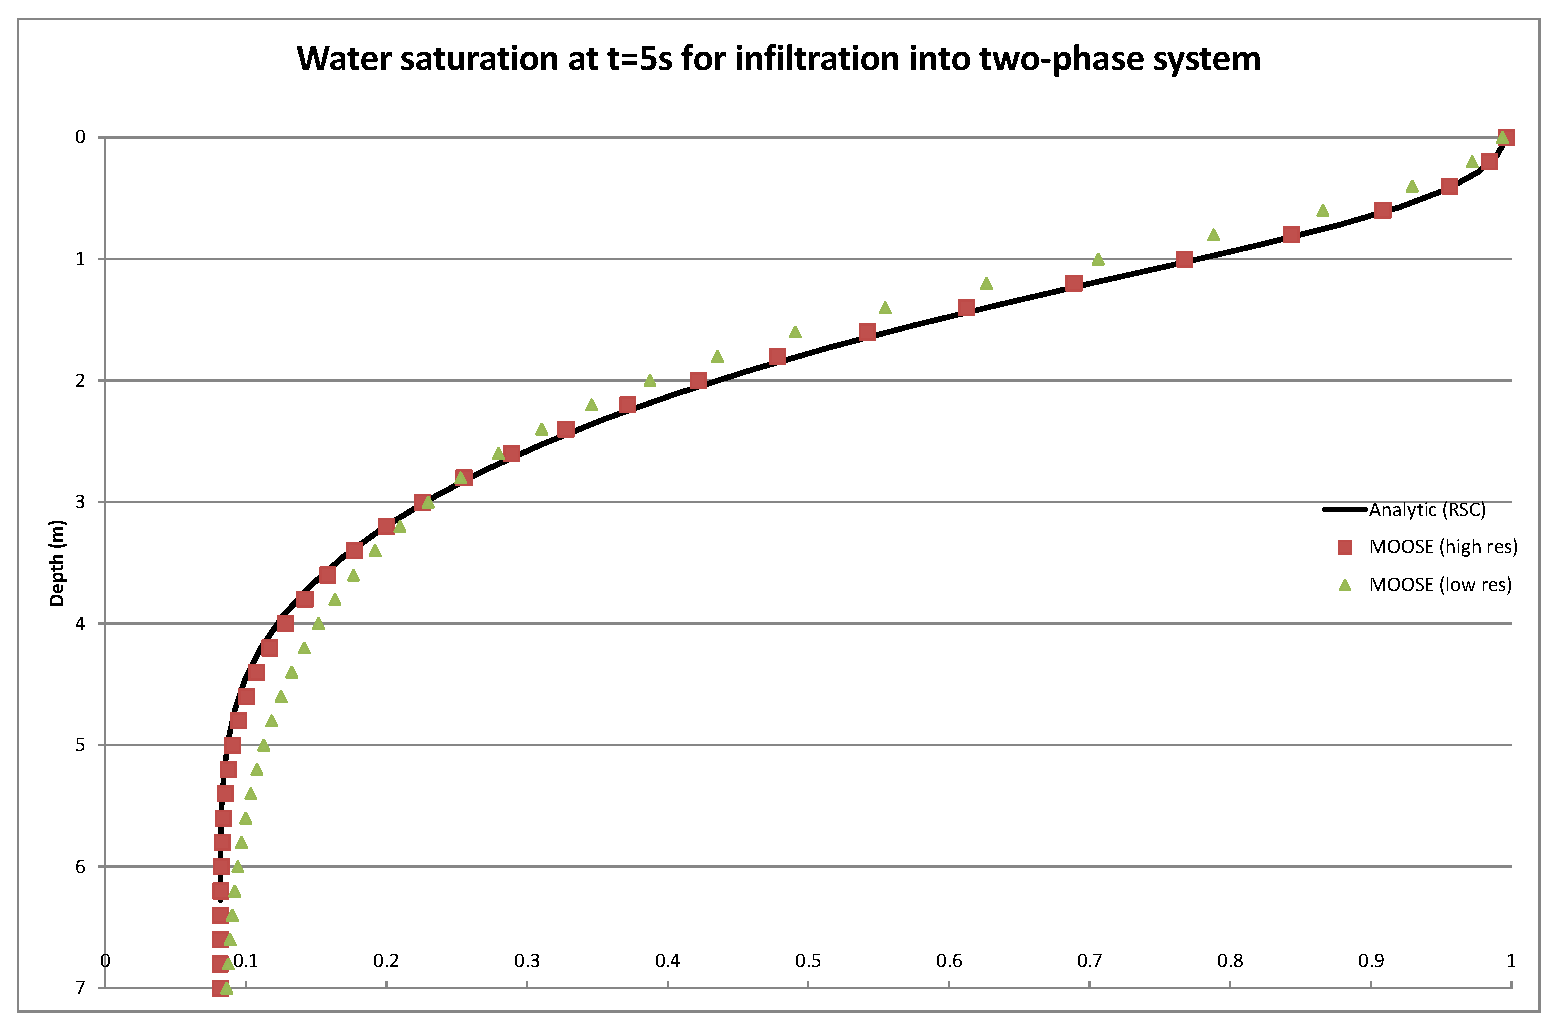
\includegraphics[width=16cm]{rsc.eps}
\caption{Water saturation profile for $t=5$\,s in the
  Rogers-Stallybrass-Clements test.  The initial water saturation is
  0.08181, and water is injected at the top of this figure at a
  constant rate.  This forms a water front which displaces the oil.
  Black line: RSC's analytic solution.  Red squares: high-resolution
  MOOSE simulation.  Green triangles: lower resolution MOOSE simulation.}
\label{rsc.fig}
\end{center}
\end{figure}







\chapter{The two-phase Buckley-Leverett problem}
\label{bl2}

MOOSE is compared with a simple two-phase one-dimensional
Buckley-Leverett problem\footnote{SE Buckley and MC Leverett (1942)
  ``Mechanism of fluid displacements in sands''.  Transactions of the
  AIME {\bf 146} 107--116}.  The fluids move in a region
$0\leq x\leq 15$\,m.  A water-saturated front initially sits at
position $x=5$, while the region $x>5$ is initially water-unsaturated.
The water pressure is high in the region $x<5$.  With very small
capillary suction function $P_{c} \sim 0$, there is virtually no
diffusion of the sharp front, and it progresses towards the right,
driven by the high water pressure.  This is a difficult problem to
simulate numerically as maintaining the sharp front is hard.
Moreoever, because it is impossible to use $P_{c}=0$ in the MOOSE
implementation, it is necessary to use large porepressure changes
around the front to create the front.  This is
difficult to handle numerically.  The front's speed is independent of
the relative permeability, since the fluid is flowing from a
fully-saturated region (where $\kappa_{\mathrm{rel}}=1$).


In the simulations below, the water pressure at the left boundary is
kept fixed at $P_{0}=1$\,MPa, while the right boundary is kept fixed
at $P_{15}=-10^{5}$\,Pa.  The water viscosity is $\mu = 10^{-3}$\,Pa.s.  In
order to correspond as closely as possible to the single-phase version
of this test (Chapter~\ref{bl}), the gas-phase viscosity is set to
$10^{-6}$\,Pa.s.  This means it interferes very little in the
progression of the water front.

The parameters used are listed below
\begin{center}
\begin{tabular}{|ll|}
\hline
Porosity & 0.15 \\
Permeability & $ 10^{-10}$\,m$^{2}$ \\
\hline
Water base density & 1000\,kg.m$^{-3}$ \\
Water viscosity & $10^{-3}$\,Pa.s \\
Water bulk modulus & 2\,MPa \\
Water relative perm power & 2 \\
Water immobile saturation & 0.0 \\
Water residual saturation & 0.0 \\
\hline
Gas base density & 1\,kg.m$^{-3}$ \\
Gas viscosity & $10^{-6}$\,Pa.s \\
Gas bulk modulus & 2\,MPa \\
Gas relative perm power & 2 \\
Gas immobile saturation & 0.0 \\
Gas residual saturation & 0.0 \\
\hline
van Genuchten $\alpha$ & $10^{-4}$\,Pa$^{-1}$ \\
van Genuchten $m$ & 0.8 \\
\hline
\end{tabular} \\
\end{center}


The initial condition is
\begin{equation}
P_{\mathrm{water}}(t=0) = \left\{
\begin{array}{ll}
10^{6}(1-x/5) & \ \ \ \mbox{for }\ \ x<5 \\
-10^{5} & \ \ \ \mbox{for }\ \ x\geq 5  
\end{array}
\right. \ ,
\end{equation}
and
\begin{equation}
P_{\mathrm{gas}}(t=0) = \left\{
\begin{array}{ll}
10^{6}(1-x/5) + 10^{3} & \ \ \ \mbox{for }\ \ x<5 \\
10^{3} & \ \ \ \mbox{for }\ \ x\geq 5  
\end{array}
\right. \ .
\end{equation}
which is shown in Figure~\ref{bl2_setup.figa}.  Using a slighly higher
$P_{\mathrm{gas}}$ than $P_{\mathrm{water}}$ makes the problem more
stable, as the gas equations do not vanish in the saturated zeon.
With the suction function defined above this gives
\begin{equation}
S(t=0) = \left\{
\begin{array}{ll}
1 & \ \ \ \mbox{for }\ \ x < 5 \\
10^{-4} & \ \ \ \mbox{for} \ \ x \geq 5  \ ,
\end{array}
\right.
\end{equation}
to within $10^{-6}$.

\begin{figure}[htb]
\begin{center}
\includegraphics[width=12cm]{bl2_initial.eps}
\caption{Initial setup of the Buckley-Leverett problem where
  porepressure is a piecewise linear function.  The region
$x<5$ is fully water saturated, while the region $x>5$ has saturation
  $10^{-4}$.  During simulation the values of porepressure at the end
  points are held fixed.}
\label{bl2_setup.figa}
\end{center}
\end{figure}

The porepressures at the end and right of the model are held fixed.

Good approximations for the water pressure $P(x,t)$
and the front position $f(t)$ may be determined from
\begin{eqnarray}
\frac{{\mathrm d} f}{{\mathrm d} t} & = & -\frac{\kappa}{\phi\mu_{\mathrm{water}}}
\left.\frac{\partial  P}{\partial x}\right|_{x = f} \ , \nonumber \\
P(x,t) & = & P_{0} - (P_{0}-P_{f})x/f \ \ \ \mbox{ for } x\leq f  \ ,
\ ,
\label{eqn.predicted.bl2.posn.eqna}
\end{eqnarray}
where $P_{f}$ is the water porepressure at the front ($P_{f}=0$)
which has solution
\begin{equation}
f(t) = \sqrt{f(0)^{2} + \frac{2\kappa}{\phi\mu_{\mathrm{water}}}(P_{0}-P_{f})t} \ .
\end{equation}
For the parameters listed above, the front will be at position
$f=9.6$\,m at $t=50$\,s.  This solution is only valid for zero
capillary suction.  A nonzero suction function will tend to diffuse
the sharp front.

Figure~\ref{satfront2.figa} shows the results from two MOOSE
simulations which validate the MOOSE implementation of two-phase fluid
flow.  Four simulations in total are part of the test suite:
\begin{enumerate}
\item ``High res''.  A uniform mesh of size 0.1\,m, with timestep between
  $10^{-4}$\,s and 0.2\,s.  The van Genuchten
  $\alpha=10^{-4}$\,Pa$^{-1}$ and $m=0.8$.  At $t=50$\,s the mesh sits
  between $x=9.6$\,m and $x=10.2$\,m.  One simulation uses mass
  lumping while the other does not.  These simulations use 833
  timesteps and take 1\,minute
  to run, so are marked as ``heavy'' in the test suite and are not run
  every time the code is updated.
\item ``Low res''.  A uniform mesh of size 0.5\,m, with timestep between 0.1\,s and
  4\,s.  The van Genuchten 
  $\alpha=10^{-5}$\,Pa$^{-1}$ and $m=0.8$.  Instead of $P=-10^{5}$\,Pa
  at the $x=15$ end, $P=-3\times 10^{5}$\,Pa is used instead, which
  means $s=0.01$ in the unsaturated zone.  At $t=50$\,s the mesh sits
  between $x=9.3$\,m and $x=12.3$\,m.  One simulation uses mass
  lumping while the other does not.  These simulations uses 37
  timesteps and take 0.7\,seconds to run, so are part of the automatic
  test suite.
\end{enumerate}
Mass lumping removes the oscillatory behaviour of the solution, as
shown in Figure~\ref{bl_lump.fig}.



\begin{figure}[htb]
\begin{center}
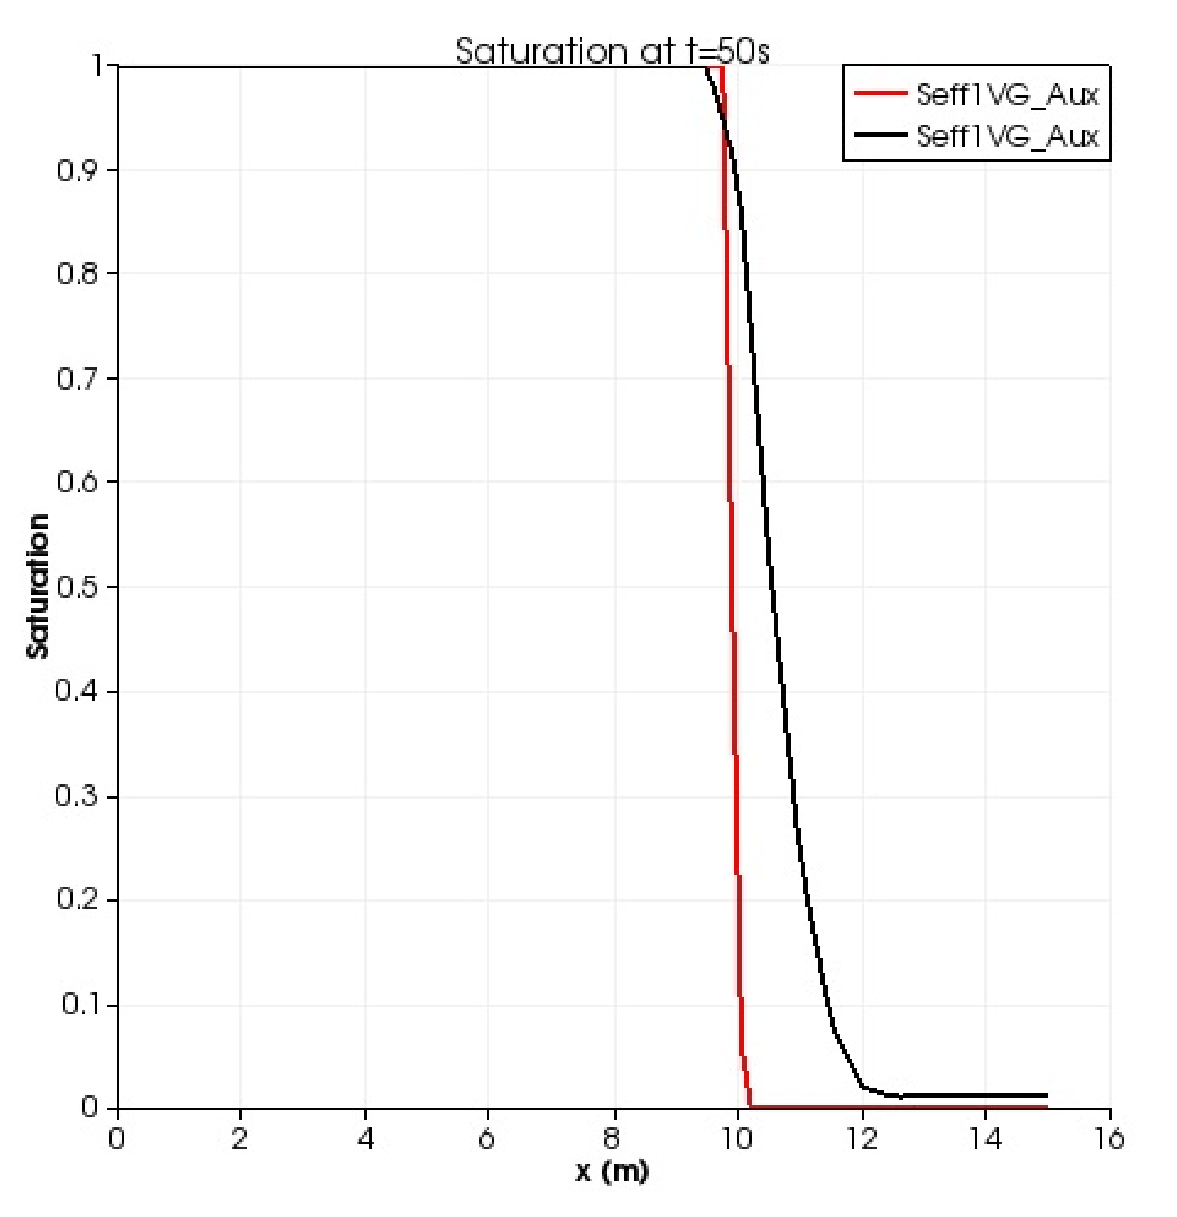
\includegraphics[width=10cm]{bl2_seff.eps} \\
$\mbox{}$
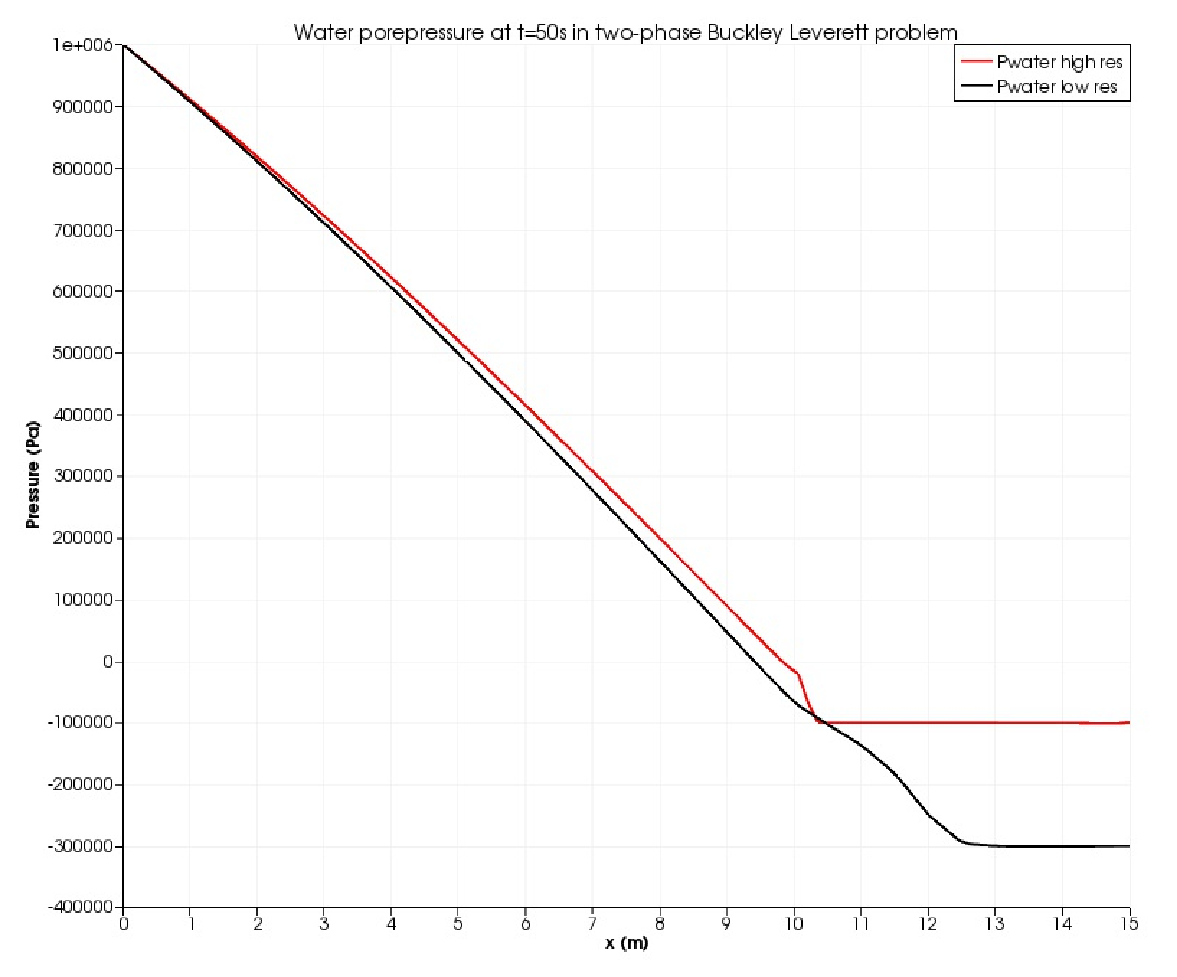
\includegraphics[width=10cm]{bl2_p.eps} \\
\caption{The MOOSE solution of the two-phase Buckley-Leverett problem at
  $t=50$\,s.  Top: saturation.  Bottom: water porepressure.  The red line in
  each is the large $\alpha=10^{-4}$\,Pa$^{-1}$, and the black line is
  the $\alpha=10^{-5}$\,Pa$^{-1}$.  Both these simulations utilise
  mass lumping.}
\label{satfront2.figa}
\end{center}
\end{figure}

\begin{figure}[htb]
\centering
\begin{tabular}{cc}
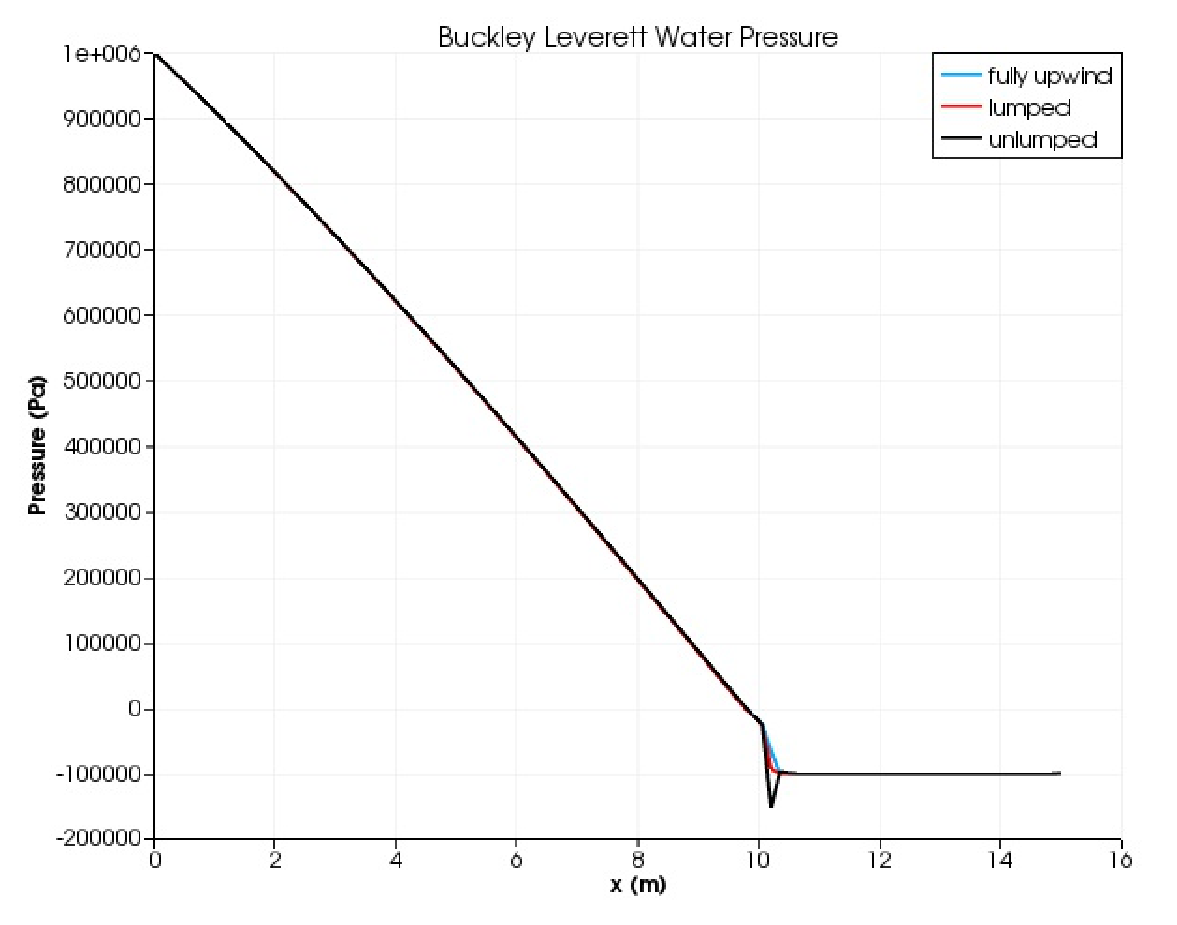
\includegraphics[width=7cm]{bl_lumped_unlumped.eps} &
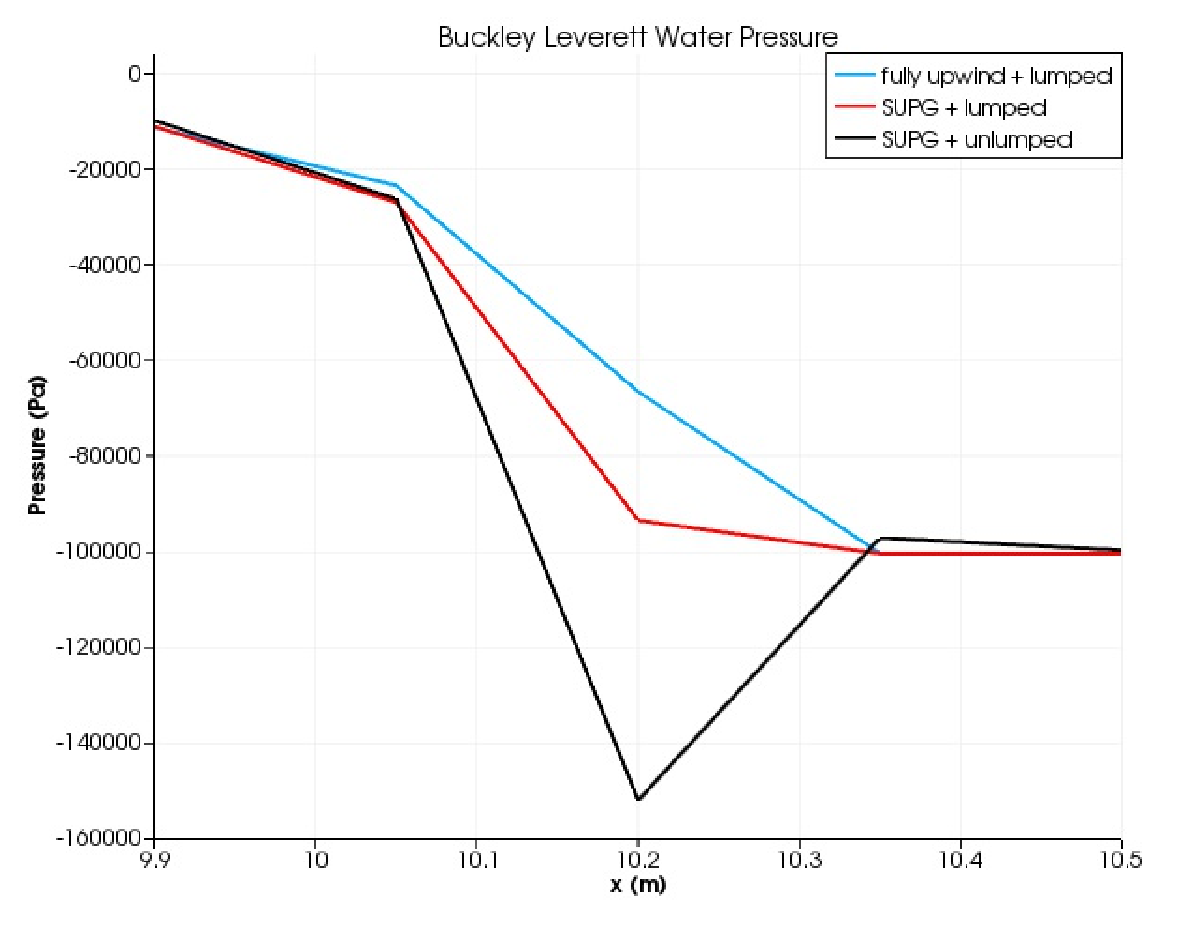
\includegraphics[width=7cm]{bl_lumped_unlumped_zoom.eps}
\end{tabular}
\caption{Comparison of the two-phase Buckley-Leverett solution at
  $t=50$\,s with and without mass lumping for the ``high res'' case
  with $\alpha = 10^{-4}$\,Pa$^{-1}$.  Note the oscillatory
  behaviour in the unlumped version.}
\label{bl_lump.fig}
\end{figure}




%\chapter{Unsaturated flow in a bar - NEEDS UPDATE}
%
%This problem is one of cosflow's benchmark problems.  Water inside a
%porous ``bar'' of material length 10m, and width and depth 1m is
%initialised to porepressure $P_{0}<0$, corresponding to water
%saturation $S_{0}<1$.  The porepressure left-hand end (at $x=0$) is
%raised and fixed at $P_{1}<0$, corresonding to water saturation
%$S_{1}$ with $S_{0}<S_{1}<1$, and the evolution of porepressure at the
%right-hand end ($x=10$\,m) is recorded.  Apart from the left-hand end,
%the other boundaries of the bar are impermeable.  The setup is shown in
%Figure~\ref{uf_setup.fig}.
%
%\begin{figure}[htb]
%\begin{center}
%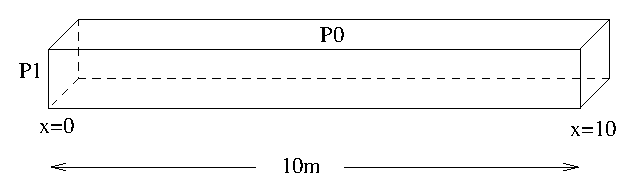
\includegraphics[width=8cm]{uf_setup.eps}
%\caption{The unsaturated problem involves a porous
%  ``bar'' of material of length 10m with initial porepressure
%  $P_{0}$.  The left-hand end is raised to porepressure $P_{1}$ and
%  held fixed.  The other parts of the bar's exterior surface are impermeable.}
%\label{uf_setup.fig}
%\end{center}
%\end{figure}
%
%This problem exhibits quite severe mesh dependency, and since the
%upwinding in cosflow and Wallaby are different, the results are not
%expected to be the same, except in the limit of zero element size.
%
%\noindent The following parameters are used \\
%\begin{center}
%\begin{tabular}{|ll|}
%\hline
%Bar porosity & 0.1 \\
%Bar permeability & $10^{-12}$\,m$^{2}$ \\
%\hline
%Gravity & 0 \\
%\hline
%Water density & 1000\,kg.m$^{-3}$ \\
%Water viscosity & 0.001\,Pa.s \\
%Water bulk modulus & 2\,GPa \\
%Water immobile saturation & 0.0 \\
%Water residual saturation & 0.0 \\
%Air residual saturation & 0.0 \\
%\hline
%van Genuchten $\alpha$ & $10^{-4}$\,Pa$^{-1}$ \\
%van Genuchten $a$ & 0.35 \\
%\hline
%Initial porepressure $P_{0}$ & -197347.0503\,Pa \\
%Initial saturation $S_{0}$ & 0.2 \\
%Applied pressure $P_{1}$ & -9283.000501\,Pa \\
%Applied saturation $S_{1}$ & 0.8 \\
%\hline
%\end{tabular} \\
%\end{center}
%
%Figure~\ref{uf.result.fig} shows agreement between Wallaby and
%cosflow for a variety of different mesh densities, including an
%adaptive mesh example.  The Wallaby results appear to be closer to the
%zero-element-size result than cosflow, but for low mesh density
%exhibit spurious oscillations as the high saturation region moves into
%the low saturation region.  (This oscillation is almost definitely due
%to my current inability to lump the mass term.)
%
%\begin{figure}[htb]
%\begin{center}
%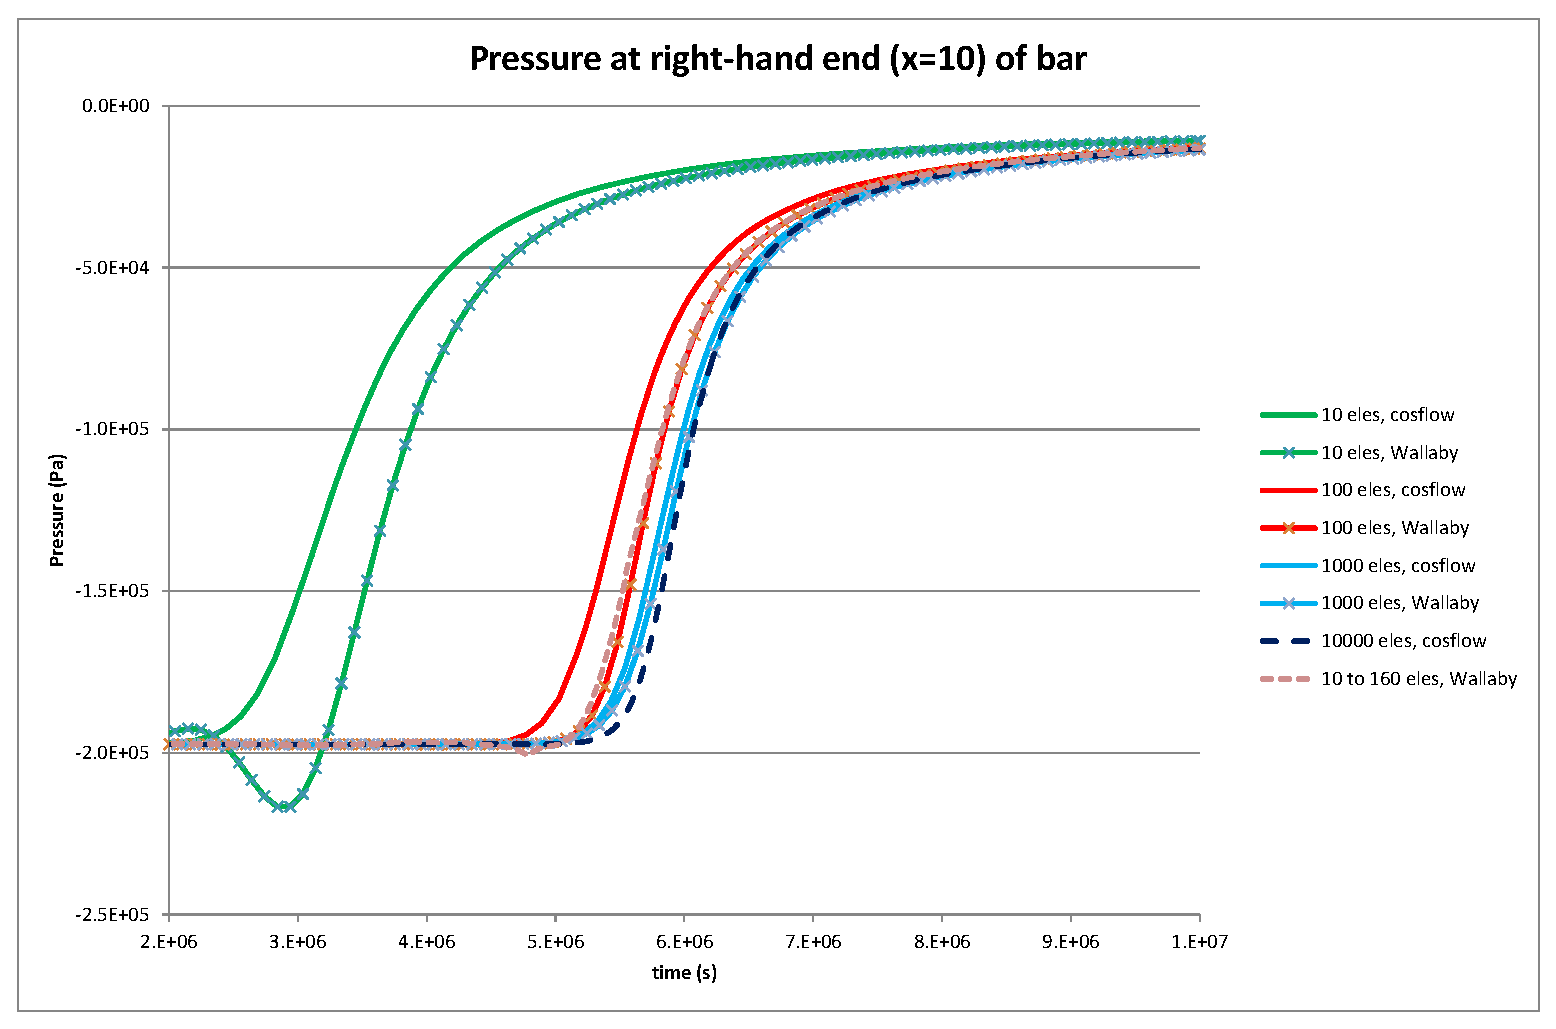
\includegraphics[width=17cm]{uf.eps}
%\caption{The porepressure at the right-hand end ($x=10$) of the bar as
%  a function of time for various different meshes.}
%\label{uf.result.fig}
%\end{center}
%\end{figure}







\end{document}

